%\documentclass[pdftex,a4paper,12pt]{scrreprt}
\documentclass[pdftex,a4paper,12pt]{scrreprt}
\usepackage{algorithm}
\usepackage{algorithmicx}
\usepackage{algpseudocode}
\usepackage{bm}

\usepackage{ngerman}
%\documentclass[pdftex,a4paper,12pt]{scrbook}
\usepackage[latin1]{inputenc} 
%\usepackage[utf8]{inputenc} 
\usepackage[bibcomment]{tntdasa}
\usepackage{hyperref}
\usepackage{graphicx}
\usepackage{subfigure}
\usepackage{enumerate}
\usepackage{pdflscape}
\usepackage{booktabs}
\usepackage{url}

\usepackage{array}
\usepackage{mathtools}
\usepackage{makeidx}
\usepackage{times}
\usepackage{amssymb}
\usepackage{amsmath}
%\hyphenation{german}
\usepackage{inputenc}

\usepackage{epstopdf}
\usepackage{mathrsfs}
\usepackage{etoolbox}

%\usepackage{hyperref}
%\usepackage{acronym}

\apptocmd{\thebibliography}{\csname phantomsection\endcsname\addcontentsline{toc}{chapter}{\bibname}}{}{}
\usepackage{float}
\usepackage{subfigure}
\usepackage[numbers]{natbib}
%\usepackage{slashbox} % make backslash in the table
\usepackage{setspace}

\usepackage{multirow}
\usepackage{units}
\usepackage{textcomp}
\usepackage{bigfoot}
\usepackage{pdflscape}
%\usepackage{hyperref}
%\hypersetup{
%           colorlinks = true,
%    linkcolor=black,        % color of internal links (change box color with linkbordercolor)
%    citecolor=red,        % color of links to bibliography
%    filecolor=magenta,      % color of file links
%    urlcolor=cyan           % color of external links
%}

 \newlength{\subfigwidth}
  \setkeys{Gin}{width=\subfigwidth}

  \def\setcols#1{%
    \setlength{\subfigwidth}{\linewidth}%
    \addtolength{\subfigwidth}{\tabcolsep}
    \addtolength{\subfigwidth}{-#1\tabcolsep}
    \divide\subfigwidth by#1}
%    
\newcommand{\argmin}{\operatornamewithlimits{argmin}}
\newcommand{\argmax}{\operatornamewithlimits{argmax}}   
 
\renewcommand{\algorithmicrequire}{\textbf{Input:}}
\renewcommand{\algorithmicensure}{\textbf{Output:}}
\renewcommand{\bibname}{Bibliography}

\renewcommand{\contentsname}{Contents}
\renewcommand{\listfigurename}{List of Figures}
\renewcommand{\listtablename}{List of Tables}
\renewcommand{\figurename}{Figure}
\renewcommand{\tablename}{Table}


\newcommand\DAGMreviewversion{
  \usepackage{lineno}
  \usepackage{color}
  \renewcommand\thelinenumber{\color[rgb]{0.2,0.5,0.8}\normalfont\sffamily\scriptsize\arabic{linenumber}\color[rgb]{0,0,0}}
  \renewcommand\makeLineNumber {\hss\thelinenumber\ \hspace{6mm} \rlap{\hskip\textwidth\ \hspace{6.5mm}\thelinenumber}} 
  \linenumbers
}
%
\pagestyle{tntdasa}

\newcolumntype{L}[1]{>{\raggedright\let\newline\\\arraybackslash\hspace{0pt}}m{#1}}
\newcolumntype{C}[1]{>{\centering\let\newline\\\arraybackslash\hspace{0pt}}m{#1}}
\newcolumntype{R}[1]{>{\raggedleft\let\newline\\\arraybackslash\hspace{0pt}}m{#1}}

%******************************************************************************
\begin{document}
%\frontmatter%
\tntdasatitle{Masterarbeit}                % Diplom/Studienarbeit
             {Dynamically Expandable Lifelong Learning: Towards Highly Transferable Adversarial Attacks for Speech Emotion Recognition Models}  % Titel der Arbeit
             {Ning Wang}    % Name des Studenten
             {Matrikelnummer: 10027258}    % Name des Studenten
             {M.Sc. Zhao Ren}    % Betreuer
             {Prof. Dr.-Ing. J"orn Ostermann}% Erstprüfer
             {Prof. Dr.-Ing. J"orn Ostermann}% Zweitprüfer
             {Hannover, Mai 2022}         % Ort,Datum (Titelseite) 
             {Hannover, den 13.05.2022}    % Ort,Datum (Erklärung)


%******************************************************************************
\setlength{\oddsidemargin}{1cm}
\setlength{\evensidemargin}{-1cm}
%******************************************************************************


\chapter*{Abstract}
\label{chap:Abstract}
\addcontentsline{toc}{chapter}{Abstract}
\setcounter{page}{1}
\pagenumbering{roman}
%******************************************************************************
In recent studies, well-designed adversarial attacks can easily fool deep Speech Emotion Recognition (SER) models into misclassifications. The transferability of adversarial attacks is a crucial evaluation indicator when generating adversarial examples to fool a new target model or multiple target models. However, to enhance the attacker's transferability, multi-task learning may require a large memory space and transfer learning may result in that an attacker forgets the knowledge from prior target models. Different from multi-task learning and transfer learning, lifelong learning can save more memory space than conventional multi-task learning and keep the attacker to deceive all target models.
In this thesis, a novel lifelong learning approach refer to as Dynamically Expandable Network (DEN), is applied to train black-box adversarial attacks for deceiving multiple target SER models. Specifically, the black-box adversarial attacks generate adversarial examples with an atrous convolutional neural network. Firstly, an adversarial attack model is trained on the first target model. Then, the trained attacker is adapted to a new target model using DEN. The DEN can dynamically adapt its network capacity as it trains on a sequence of tasks, to learn a compact overlapping knowledge sharing structure among tasks. DEN is efficiently trained in an online manner by performing i) selective retraining, ii) dynamically expanding network capacity upon arrival of each task with only the necessary number of units, and iii) effectively preventing semantic drift by splitting units. 



%In this thesis we mainly discuss  the solutions for visual relation detection. To find the solutions, we not only need to  develop models that detect the objects in an image, but also need to predict the interactions between the detected objects. Therefore, a comprehensive scene understanding of an image would be considered in aspect of connecting computer vision and natural language  helpful. Even though the work in area of deep learning has been quite successful, it remains to be a complex and challenging task to extract related scene information. 
%
% Inspired by the contemporary achievement of transformer in computer vision, we propose Retina Net, which was based transformer structure. In order to meet different requirements in visual relation detection, we designed specific object queries with physical meanings. The specific object queries is capable of extracting better object features in an image with the help of our attention loss.  By considering the global context, we also model relation to object interactions through the relation decoder. We attempt a lot to find the mechanism of attention in the models and to understand which details should be paid more attention to when it comes to relation predicts.
% 
% To our best effort, our study for the first time try to complete all the models of relation detection . It is a new approach to solve the problems by using transformer structure. The results of our experiments indicate that our models solve the tasks in visual relation detection properly.

%------------------------------------------------------------------------
%-------------------------------------------------------------------------

%******************************************************************************
\chapter*{Kurzfassung}

%------------------------------------------------------------------------
%-------------------------------------------------------------------------

%******************************************************************************
\label{chap:Kurzfassung}
\addcontentsline{toc}{chapter}{Kurzfassung}

In neueren Studien k"onnen gut konzipierte gegnerische Angriffe Deep Speech Emotion Recognition (SER)-Modelle leicht zu Fehlklassifizierungen t"auschen. Die "Ubertragbarkeit gegnerischer Angriffe ist ein entscheidender Bewertungsindikator bei der Generierung gegnerischer Beispiele, um ein neues Zielmodell oder mehrere Zielmodelle zu t"auschen. Um jedoch die "Ubertragbarkeit des Angreifers zu verbessern, kann Multi-Task-Lernen einen grossen Speicherplatz erfordern und Transfer-Lernen kann dazu f"uhren, dass ein Angreifer das Wissen aus fr"uheren Zielmodellen vergisst. Anders als Multi-Task-Lernen und Transfer-Lernen kann lebenslanges Lernen mehr Speicherplatz sparen als herk"ommliches Multi-Task-Lernen und den Angreifer dazu bringen, alle Zielmodelle zu t"auschen.

In dieser Arbeit wird ein neuartiger Ansatz des lebenslangen Lernens, der als Dynamically Expandable Network (DEN) bezeichnet wird, angewendet, um Black-Box-Attacken zu trainieren, um mehrere Ziel-SER-Modelle zu t"auschen. Insbesondere die gegnerischen Black-Box-Angriffe erzeugen gegnerische Beispiele mit einem atrous Convolutional Neural Network. Zuerst wird ein gegnerisches Angriffsmodell auf das erste Zielmodell trainiert. Dann wird der trainierte Angreifer mit DEN an ein neues Zielmodell angepasst. Das DEN kann seine Netzwerkkapazit"at dynamisch anpassen, während es eine Abfolge von Aufgaben trainiert, um eine kompakte, sich "uberschneidende Wissensteilungsstruktur zwischen Aufgaben zu lernen. DEN wird effizient online trainiert, indem i) selektives Neutraining durchgeführt wird, ii) die Netzwerkkapazit"at beim Eintreffen jeder Aufgabe nur mit der erforderlichen Anzahl von Einheiten dynamisch erweitert wird und iii) semantisches Driften durch Aufteilen von Einheiten wirksam verhindert wird.
%*******************************************************************************************

%*****************************************************************************************
\tableofcontents

\addcontentsline{toc}{chapter}{List of Tables}
\listoftables

\addcontentsline{toc}{chapter}{List of Figures}
\listoffigures
%\addtocontents{lof}{\bfseries\Large Figures\vskip10pt}
%\caption[Short version for listoffigures]
%****************************************************************************************

\hypersetup{
    colorlinks = true,
    linkcolor=blue,          % color of internal links (change box color with linkbordercolor)
    citecolor=red,        % color of links to bibliography
    filecolor=magenta,      % color of file links
    urlcolor=cyan           % color of external links
}
%========================================================================================


\chapter{Introduction}
\label{chap:introduction}
\setcounter{page}{1}
\pagenumbering{arabic}

With the development of artificial intelligence, Speech Emotion Recognition (SER) has become an important component of Human-Computer Interaction (HCI)~\cite{ZhangHJ14-3} and beyond. Recently, deep learning has emerged as a promising technique for training more robust models by extracting highly abstract representations compared to traditional big data machine learning approaches~\cite{triantafyllopoulos2019towards}. A range of deep learning topologies have been successfully applied to SER tasks, such as Convolutional Neural Networks (CNNs)~\cite{trigeorgis2016adieu} and Recurrent Neural Networks (RNNs)~\cite{zhao2019exploring}.
According to recent studies, deep learning models are vulnerable to external adversarial attacks~\cite{ren2020enhancing}, where the generated examples have a high degree of similarity to real data.
This naturalness can be achieved by adding minimal and well-designed perturbations. In addition, adversarial samples can make deep learning models susceptible to misclassification. In particular, adversarial attacks have the potential to pose a threat to SER systems, resulting in invalid and misinterpreted interactions with users~\cite{ren2020generating}. For example, adversarial attacks may even be life-threatening in the case of misdiagnosis of emotion-related psychiatric disorders, e.g. g., depression~\cite{ringeval2019avec} and bipolar disorder~\cite{ren2019multi}.

\section{Motivation}

Generating artificial adversarial samples to simulate the attack process is an important step in preventing real-world attacks. This also helps to further improve the robustness of the targeted deep learning model~\cite{samangouei2018defense}. In this regard, a series of research works aim to construct white-box and black-box adversarial attacks~\cite{ren2020enhancing,madry2017towards}. White-box attacks require data sources and
complete parameters within the target model, while the data or parameters are blind in black-box attacks~\cite{madry2017towards}. While examples of white-box attack generation can be induced by gradient descent methods~\cite{ren2020enhancing}, searching for black-box attacks without knowledge or partial knowledge of the target model is challenging. Improving the transferability of black-box adversarial attacks
Facilitates the generation of stronger adversarial data that are transferable between different target models~\cite{liu2017delving}. Highly transferable adversarial attacks can deceive not only already deployed target models but also new target systems~\cite{wu2018understanding}.
Improved transferability can also help save costs associated with learning a unified attacker compared to training independent attackers for each target model. While attacking target models is often considered as a single task, multi-task learning~\cite{zhao2018data,zhang2019attention} optimizes attackers to deceive multiple target models simultaneously. However, training multiple tasks increases the complexity in time and space. Transfer learning~\cite{wang2018great} can help fine-tune the attacker to obtain new target models using prior knowledge gained from the previous target; however, the attack model gradually forgets the prior knowledge. Inspired by the lifelong learning paradigm~\cite{parisi2019continual}, we propose for the first time, to the authors' knowledge, to improve the transferability of black-box adversarial attacks by exploiting the lifelong learning framework.
Lifelong learning constrainedly migrates prior knowledge and thus promises to overcome the drawbacks of multitasking and migratory learning by adapting the attack model to a new target model, reducing time and memory, and not forgetting prior knowledge. With this goal in mind, this paper aims to improve the transferability of non-targeted black-box adversarial attacks for deep SER models.
 
\section{Contribution}

In this thesis, we provide a framework based on dynamically extended networks for lifelong learning of attack models. The main work and contributions are summarized as follows:
\begin{enumerate}[\qquad  1.]
	\item The approach of dynamically expanding networks is successfully applied to the attack model for adversarial networks, enabling lifelong learning.
	\item Demonstrates that a lifelong learning approach can be effective for multiple tasks simultaneously.
	\item Achieves better results for simultaneous multi-task attacks.
\end{enumerate}


\section{Organization of the Thesis}
This thesis is structured as follows:

In Chapter~\ref{chap:relatedwork}, we will discuss about the related works. Some advanced researches and methods for enhancing transferability of adversarial attacks. We also demonstrate their contributions and limitations.

In Chapter ~\ref{chap:bg}, the theories about lifelong learning and attack models(CNN)and algorithm such as Regularization will be introduced. And how did signal processe.

In Chapter ~\ref{chap:framework}, the methodology(DEN) will be shown in detail.

In Chapter ~\ref{chap:experiment},the experimental results will be presented and analyzed in detail. Our proposed framework is evaluated on target models with evaluation metrics.

In Chapter ~\ref{chap:conclusion}, we conclude our work finally and point out the future research direction.
\chapter{Related Work}
\label{chap:relatedwork}
Recently, most of the research on adversarial attacks has studied image processing tasks~\cite{akhtar2018threat}, while only a few works focus on adversarial attacks on SER systems. A few works in~\cite{gong2017crafting} explore white-box attacks to spoof SER models. A Generative Adversarial Network (GAN) based approach has also been proposed to generate black-box fake data~\cite{latif2018adversarial}. The research in our paper focuses on generating black-box adversarial data to deceive deep SER models. In the experiments, we focus on the fact that the same attack model can be trained by multiple defensive models and be effective for multiple defensive models at the same time, i.e., making the accuracy of multiple defensive models decrease.

\section{Attack model:Black-box}

\subsection{Adversarial Attack}

Most of the image classification networks based on deep learning are trained under elaborate datasets and deployed accordingly, and the recognition ability of the network is often affected to some extent for images outside the dataset or slightly modified images.
Under this phenomenon, Adversarial Attack starts to join in the examination of network model robustness.
By adding different noise or modifying some regions of the image to generate adversarial samples, the samples are used to attack the network model in order to confuse the network, i.e., adversarial attack.
The added interference information does not make any difference to the human eye, but for the network model, a change in some values can cause a "one-shot" effect. This will be a very significant error in the actual application, if it happens in the field of security, security, etc., there will be incalculable problems.
Counter-attack is usually divided into white-box attacks and black-box attacks. For a white-box attack, the attacker knows all the information and parameters inside the model and generates an adversarial sample based on the gradient of the given model to attack the network. For black-box attacks, the attacker does not know the parameters and structural information of the model, and generates adversarial samples based on the inputs and outputs of the model only, and then attacks the network. The idea of both black-box and white-box attacks is to pass the gradient information in order to generate adversarial samples that can deceive the network.

\subsection{Black-box Attack}

When the attacker does not have access to the model details, white-box attacks are obviously not applicable. Black-box attacks, i.e., without knowing the parameters and structural information of the model, generate adversarial samples only through the inputs and outputs of the model, and then attack the network.
The secrecy of the corresponding system in real life is still reliable, and the information of the model is completely leaked rarely, so the white-box attack is much less than the black-box attack. However, the idea of both is the same, to pass the gradient information in order to generate adversarial samples for the purpose of deceiving the network model.
Black-box attacks are known in the literature as a way to trick neural networks into misclassifying instances, usually by adding perturbations (i.e., extra noise) to the data~\cite{ren2020generating}. In our example, let us define the input data as $x$, the target as y, and the learning parameters of a deep model (e.g., a convolutional neural network (CNN)) as $w$. We first reduce the deep model to a linear function: $y = wx$, and add a little perturbation to the input data $x$, defining the new input data as $x^{\prime}=x+\theta$. The function $y = wx$ can then be updated to $w x^{\prime}=w x+w \theta$. As the model goes deeper (i.e., additional layers), the model may produce incorrect predictions of $w x^{\prime}$ from $wx$, even though $\theta$ is very small. Similarly, the nonlinear depth model is subject to perturbations. Therefore, the generated data $x^{\prime}$ (i.e., adversarial data) may try to trick the depth model by adding adversarial noise to the original real data $x$, as shown in Figure 1.
To generate adversarial data, we used the Fast Gradient Sign Method (FGSM)~\cite{ren2020generating}, which computes the gradient as adversarial noise. The loss value during training is defined by $L(\boldsymbol{w}, \boldsymbol{x}, y)$ and the gradient $\nabla_{\boldsymbol{x}} L(\boldsymbol{w}, \boldsymbol{x}, y)$ can be obtained by backpropagation. The adversarial data can be computed by $$\boldsymbol{x}^{\prime}=\boldsymbol{x}+\epsilon * \operatorname{sign}\left(\nabla_{\boldsymbol{x}} L(\boldsymbol{w}, \boldsymbol{x}, y)\right)$$
$$\boldsymbol{x}^{\prime}=\operatorname{clip}\left(\boldsymbol{x}^{\prime}, \boldsymbol{x}-\eta, \boldsymbol{x}+\eta\right)$$where is a constant perturbation factor and $\eta$ is a constant parameter used to crop $x^{\prime}$ into the interval $[\boldsymbol{x}-\eta, \boldsymbol{x}+\eta]$. The generated dummy data can help in data augmentation while training the model and attack the pre-trained model during validation. As shown in Figure 2, the deep model can produce correct predictions for the real log-Mel spectrogram image with a probability of 0.866. However, in our example, it predicts $happiness$ with a probability of 0.958 after adding a slight adversarial noise to the original image.

\section{Methods for enhancing transferability of adversarial attacks}

In this experiment, the attack model needs to attack multiple defensive models at the same time. Therefore multi-task learning is the focus of the study, how to have better results in different defense models at the same time?
There are usually several common approaches to multi-task learning:
\begin{enumerate}[\qquad  1.]
	\item Single-task learning
	\item Multi-task learning
	\item Transfer learning
	\item Lifelong learning
\end{enumerate}

\subsection{Single-task learning}

Single-task learning is the traditional learning method, which is a classifier for a single task. Advantages of single-task learning: it can classify targets accurately and achieve high accuracy. The disadvantages are also very obvious: it is not able to learn efficiently for other tasks, wastes time and memory, and requires restarting the training each time.
For our black box attack, it is very intrusive for one task and can make the accuracy of the classifier drop significantly. But it cannot be effective for more than one task at the same time, i.e., it does not feature transfer learning. The principle is similar to this image.

\subsection{Multi-task learning}

Multitask Learning is an inductive migration learning method in which the main tasks use the domain-specific information possessed by the training signal of the related tasks~\cite{bengio2006greedy}. It is a machine learning method that uses the domain-specific information possessed by the training signal of related tasks as an inductive bias to improve the generalization performance of the main tasks. Multi-task learning involves multiple related tasks learning in parallel, with gradients back-propagating simultaneously, and multiple tasks helping each other to learn through the underlying shared representation to improve the generalization performance~\cite{collobert2008unified}. In short: multitask learning puts multiple related tasks together (note that they must be related tasks, and the definition of related tasks and the information they share will be given later), and the learning process (training) is performed through a shared representation at a shallow level to help each other The learning process (training) is based on a shared representation at a shallow level to share and complement each other's domain information, to promote each other's learning, and to improve generalization.
Advantages of multi-task learning:
\begin{enumerate}[\qquad  1.]
	\item Multiple related tasks are put together for learning, and there are related parts, but there are also irrelevant parts. When learning a task (Main task), the parts that are not relevant to the task are equivalent to noise in the learning process, so introducing noise can improve the generalization (generalization) effect of learning.
	\item In single task learning, the back propagation of gradient tends to fall into local minima. In multi-task learning, the local minima of different tasks are in different locations, which can help the hidden layer escape from the local minima by interacting with each other.
	\item The added tasks can change the dynamic characteristics of the weight update, which may make the network more suitable for multi-task learning. For example, multi-task learning in parallel improves the learning rate of the shallow shared representation layer (SHARED representation), and possibly, the larger learning rate improves the learning effect.
	\item Multiple tasks in the shallow shared representation may weaken the network, reduce network overfitting, and improve the generalization effect.
\end{enumerate}

\subsection{Transfer learning}

Pre-training + fine-tuning is a very popular transfer learning approach in deep learning, and often the pre-trained ImageNet is chosen to initialize the model.
The concept in transfer learning:
\begin{enumerate}[\qquad  1.]
	\item Domain:Generally refers to the feature space and probability distribution.
	\item Task:Includes marker space and target prediction function.
	\item Source And Target:The former is the domain/task used to train the model, and the latter is the domain/task to perform machine learning tasks such as prediction/classification/clustering on your own data using the former model.
\end{enumerate}

The types of transfer learning can be categorized according to the content of the transfer as follows:
\begin{enumerate}[\qquad  1.]
	\item Instance-based TL:The source domain data cannot be directly used in the target domain, but there are some data in the source domain that can be reused in the target domain. After adjusting the weight to match the data in the target domain, the data can be migrated.
	\item Feature-representation-transfer:Find some good representative features and transform the features of source domain and target domain to the same space by feature transformation, so that the data of source domain and target domain have the same distribution in this space.
	\item Parameter-transfer:Suppose some parameters are shared between source tasks and target tasks, or the prior distribution of model hyperparameters is shared. This can achieve good accuracy when migrating the original model to the new domain
\end{enumerate}

$Pre-training + fine-tuning transfer$ learning approach can be understood as a Parameter-transfer, and this approach is also the most commonly used application of transfer learning.The common training trick and tuning methods used in the transfer learning process in the $Pre-training + fine-tuning$ mode are summarized as follows:
\begin{enumerate}[\qquad  1.]
	\item Feature Extractor:TensorFlow or Pytorch have pre-trained models on ImageNet, and the last fully-connected layer (the original is 1000 categories or more) can be changed to the output of your own classification task, or the last layer can be directly removed and replaced with your own classifier, and the rest of the network structure can be used as a feature extractor.
	\item Fine-tuning:In general, it is not always good enough to use the pre-trained model directly, so fine-tuning is needed. fine-tuning requires freezing the parameters of the first few layers of the network and updating only the later layers of the network structure and the last fully connected layer, which will be more effective.
	\item Learning rate:It is generally not recommended to use too large a learning rate in the fine-tuning process of migration learning; usually 1e-5 is a more appropriate choice.
\end{enumerate}

The disadvantage of transfer learning is also obvious: it is easy to forget the previous knowledge (model parameters). Transfer learning will pass the previous parameters to the new model to continue training, but will not consider again the impact of the newly trained model on the previous model.

\subsection{Lifelong learning}

Lifetime learning~\cite{thrun1995lifelong}, the problem of continuous learning in which tasks arrive sequentially, is an important topic in migration learning. The main goal of lifelong learning is to exploit the knowledge from earlier tasks to obtain better performance or to obtain faster convergence/training speed on the model for later tasks. While many different approaches exist to address this problem, we consider lifelong learning under deep learning to harness the power of deep neural networks. Fortunately, for deep learning, knowledge can be stored and transferred in a straightforward manner through learned network weights. The learned weights can be used as knowledge for existing tasks, and new tasks can take advantage of this by simply sharing these weights. Thus, in the case of deep neural networks, we can consider lifelong learning simply as a special case of online or incremental learning. There are multiple ways to perform such incremental learning~\cite{rusu2016progressive}. The simplest approach is to incrementally fine-tune the network to fit the new task by continuing to train the network with new training data. However, this simple retraining of the network degrades the performance of both the new task and the old task. If the new task is very different from the old one, e.g., the previous task was to classify images of animals, while the new task is to classify images of cars, the features learned in the previous task may be useful for the new one. At the same time, retrained representations of the new task may adversely affect the old task because they may have deviated from their original meaning and no longer fit them. For example, a feature describing a zebra stripe pattern may change its meaning for a later classification task for categories such as striped T-shirts or fences, which can adapt the feature and completely change its meaning.
Recent work suggests using regularizers to prevent drastic changes in parameter values, but still find a good solution for new tasks~\cite{kirkpatrick2017overcoming} or to prevent any changes to old task parameters~\cite{rusu2016progressive}.

\chapter{Background}
\label{chap:bg}
In this chapter, We introduce the structure of the attack model(CNN), the method of sound signal processing(Mel-spectrogram), and the method of lifelong learning(Regularization). They are the basic of our framework.

\section{Convolutional Neural Network }


A Convolutional Neural Network (CNN) is a feed-forward neural network. Its artificial neurons can respond to a portion of the surrounding units in the coverage area and have excellent performance for large-scale image processing.

A convolutional neural network consists of one or more convolutional layers and a fully connected layer on top, and also includes associated weighting and pooling layers. This structure allows convolutional neural networks to use the two-dimensional structure of the input data. Compared to other deep learning structures, convolutional neural networks can give better results in image and speech recognition. The model can also be trained using a back propagation algorithm. Convolutional neural networks require fewer parameters to be considered than other deep feed-forward neural networks, making them an attractive deep learning structure.

\subsection{Convolutional Layers}

Each convolutional layer in a convolutional neural network consists of several convolutional units, and the parameters of each convolutional unit are optimized by a backpropagation algorithm. The purpose of the convolution operation is to extract different features of the input. The first convolutional layer may extract only some low-level features such as edges, lines, and corners. More layers of the network can iteratively extract more complex features from the low-level features. For example, using a 3x3 convolution kernel requires only 9 learnable parameters since each region has the same shared weights, regardless of the size of the input image. Using regular weights on fewer parameters avoids the gradient disappearance and gradient explosion problems that can occur during backpropagation.

\begin{figure}[H]
	\centering
	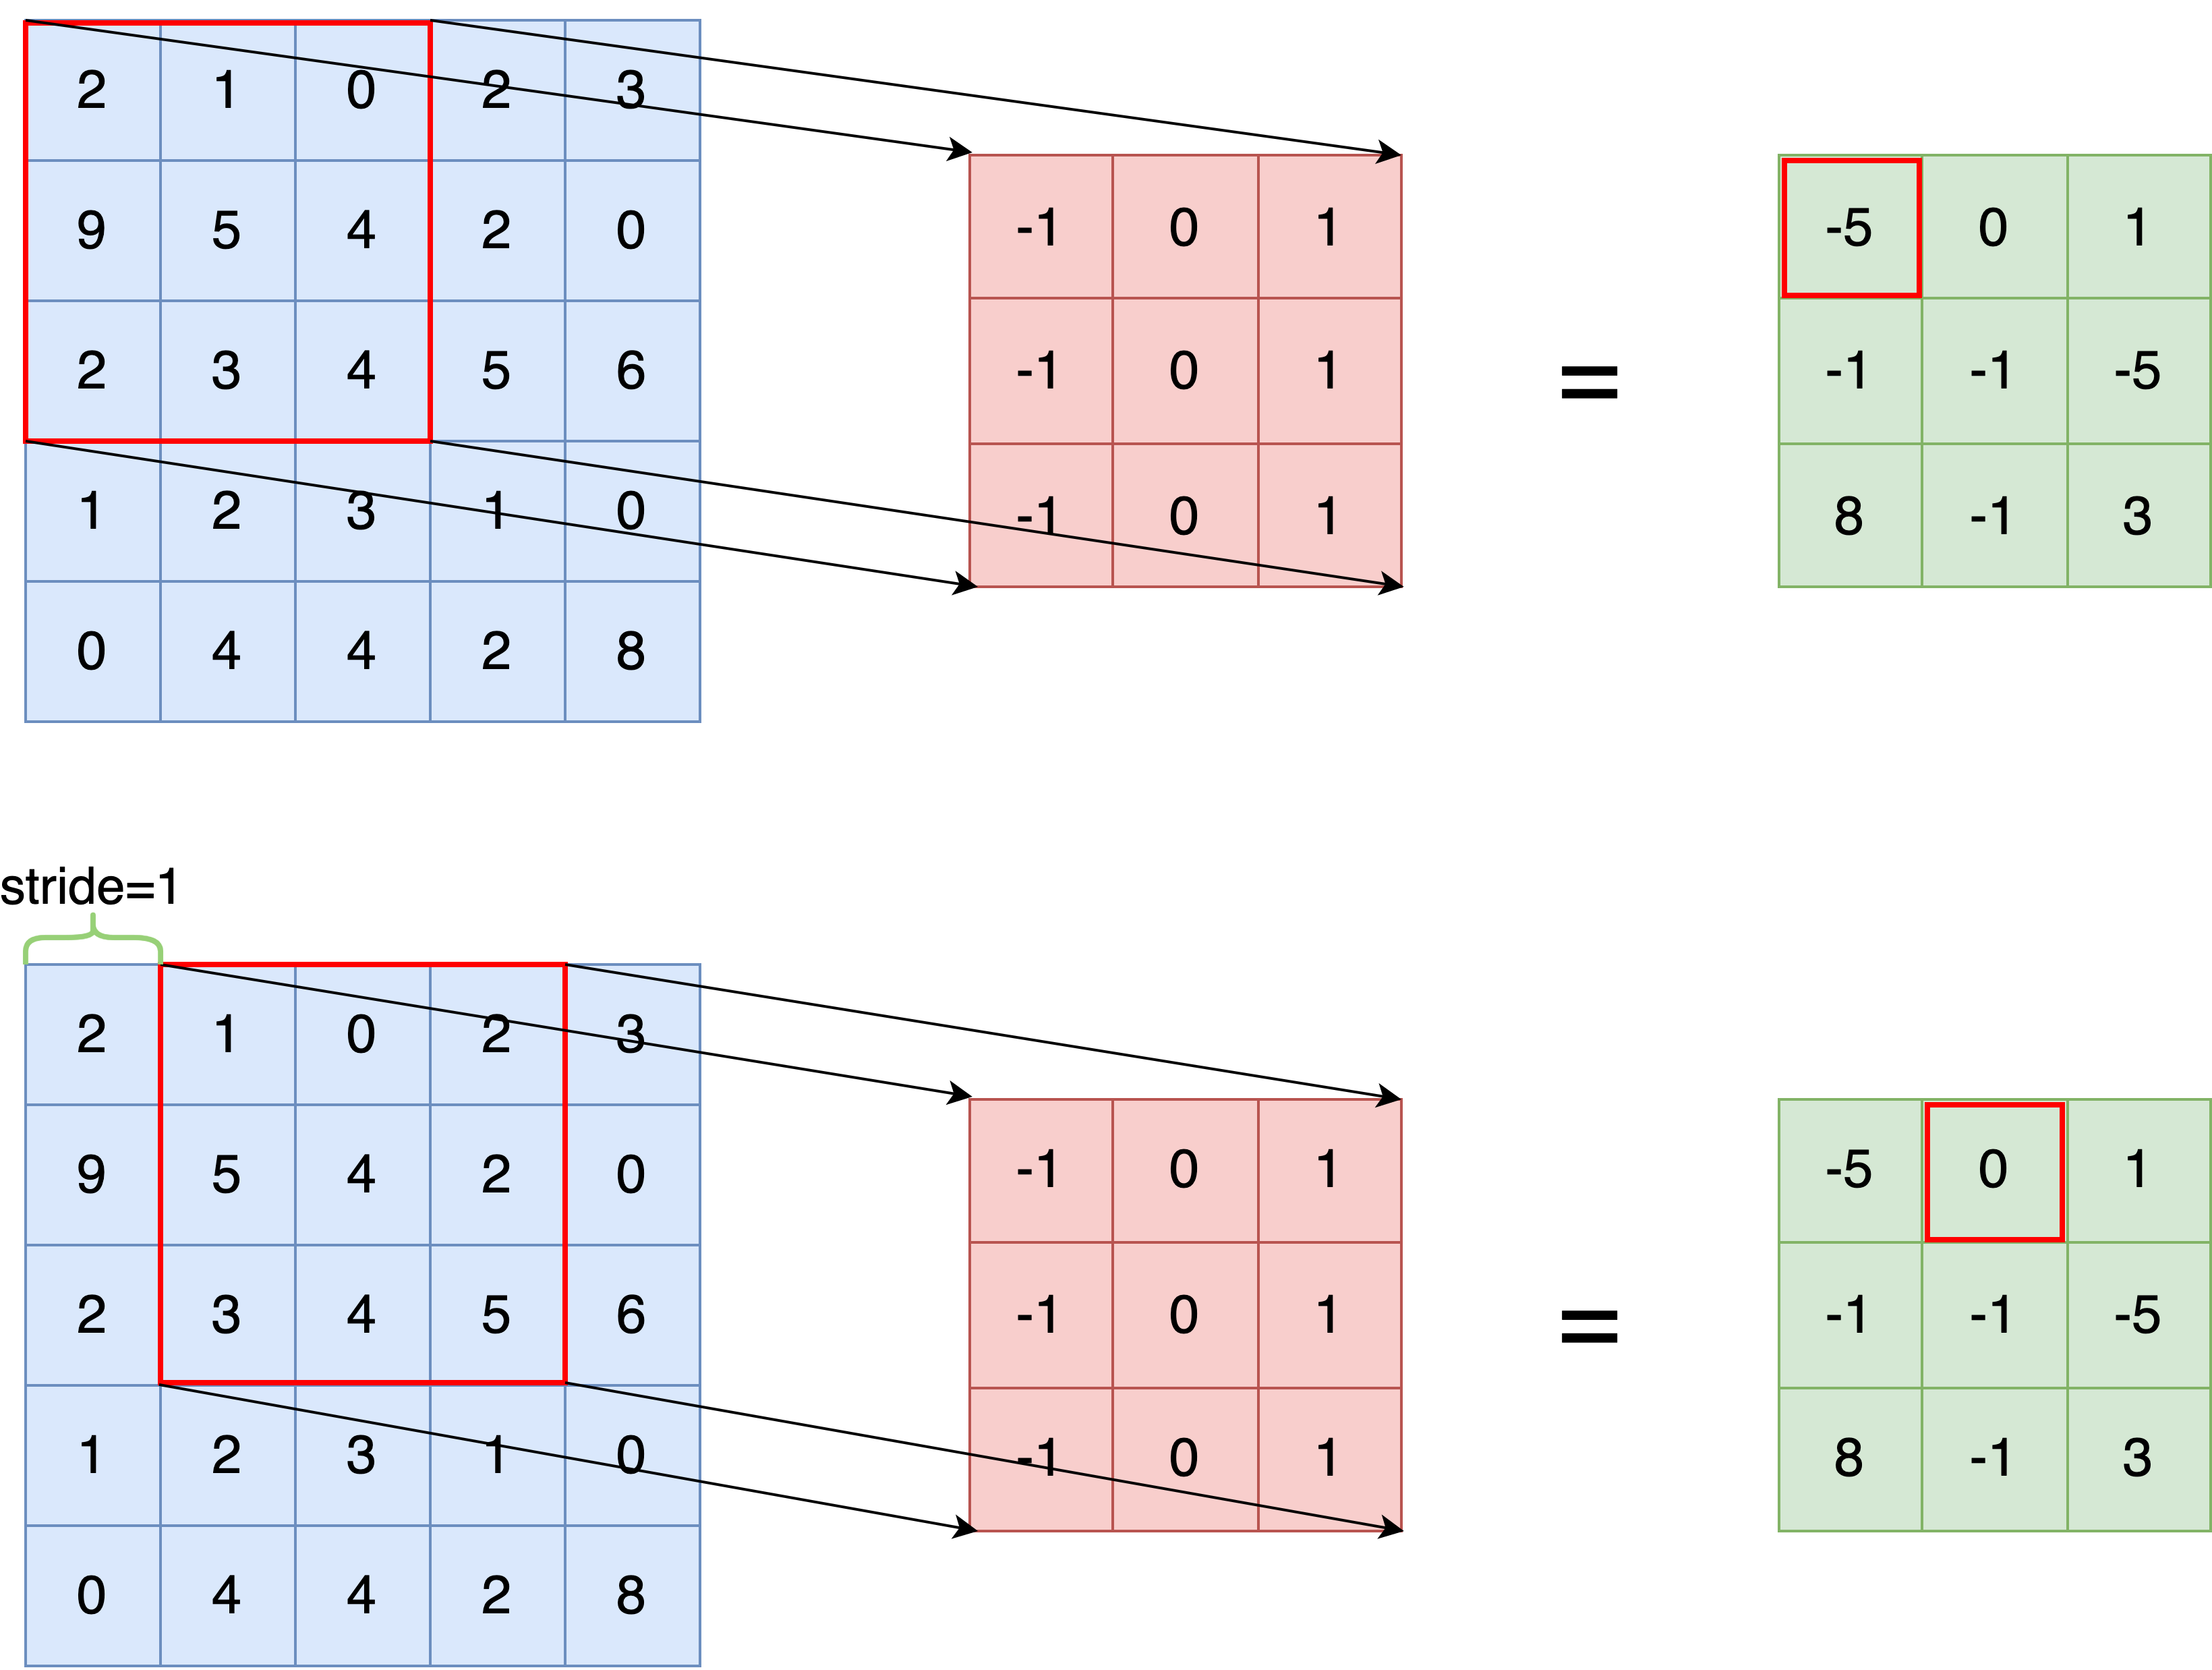
\includegraphics[width=0.6\linewidth]{figures/conv}
	\caption[An example of two-dimensional convolution]{A simple two dimensional convolution with a 3x3 convolutional kernel and stride = 1, the output size is 3x3 which is decided by image size, kernel size and stride.}
	\label{fig:conv}
\end{figure}

\subsection{Pooling Layers}

Pooling is also important concept in convolutional neural networks, and it is actually a form of downsampling. There are many different forms of nonlinear pooling functions, of which maximum pooling (see Figure ~\ref{fig:maxpool} for an example) is the most common. It divides the input image into several rectangular regions and outputs the maximum value of each subregion. Intuitively, this mechanism works because after a feature is found, its exact position is much less important than its relative position to other features. The pooling layer continuously reduces the size of the data space, so the number of parameters and the amount of computation are also reduced, which also controls overfitting to some extent. Usually, the pooling layer is inserted periodically between the convolutional layers of the CNN.

\begin{figure}[H]
	\centering
	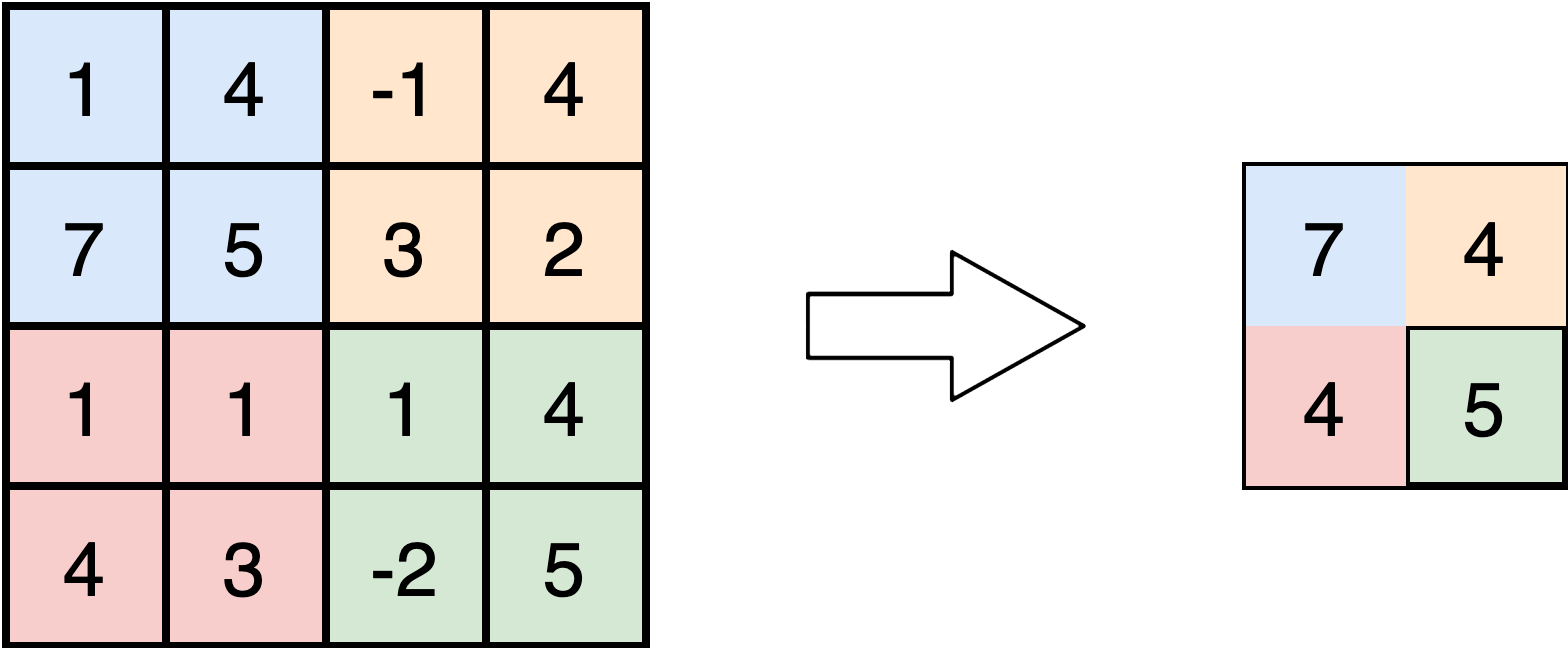
\includegraphics[width=0.6\linewidth]{figures/maxpool}
	\caption[An example of max pooling]{An example of max pooling with a 2x2 kernel and the stride is 2.}
	\label{fig:maxpool}
\end{figure}

\subsection{Fully Connection Layers}

In a CNN structure, one or more fully connected layers are connected after multiple convolutional and pooling layers. Similar to a multilayer perceptron (MLP), each neuron in a fully connected layer is fully connected to all neurons in the previous layer. The fully connected layers can combine local information with category differentiation in the convolutional or pooling layers. To improve the performance of the CNN network, the activation function of each neuron in the fully connected layer generally uses the ReLU function. The output value of the last fully connected layer is passed to an output that can be classified by softmax regression. This layer can also be referred to as a softmax layer. For a specific classification task, it is important to choose the appropriate loss function. CNNs have several commonly used loss functions, each with different characteristics. Generally the fully connected layer of CNN has the same structure as MLP, and the training algorithm of CNN mostly uses BP algorithm.
\begin{figure}[H]
	\centering
	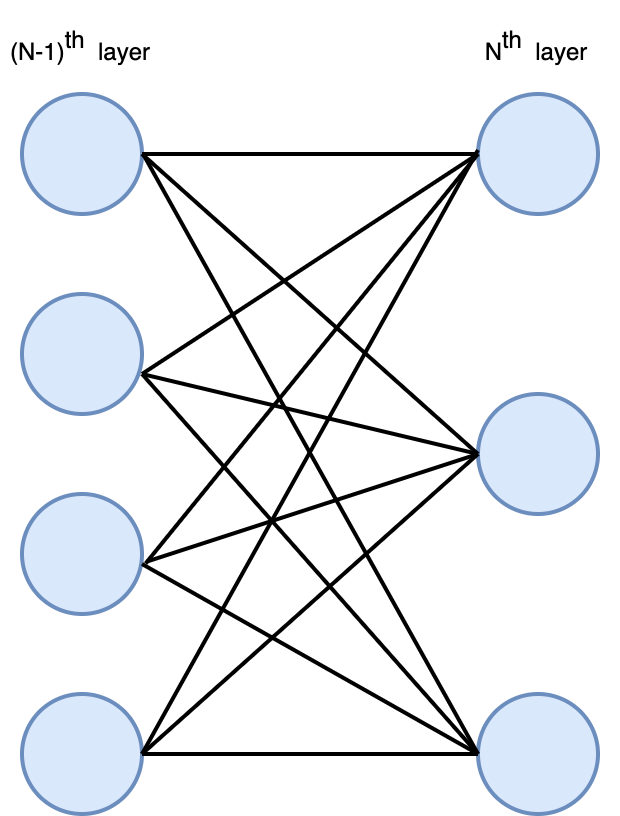
\includegraphics[width=0.4\linewidth]{figures/fc}
	\caption[The structure of fully connection layer]{The structure of fully connection layer.}
	\label{fig:fclayer}
\end{figure}


\section{Regularization Method}
\label{section:transformer}
Regularization is a general term for a class of methods in machine learning that introduce additional information to the original loss function in order to prevent overfitting and improve model generalization performance. That is, the objective function becomes the $original loss function + extra items$. There are generally two kinds of commonly used extra items, which are called $\ell 1-n o r m$ and $\ell 2-n o r m$.

\subsection{Regularized Formula}

$L1$ regularization and $L2$ regularization can be seen as penalty terms of the loss function. By penalty, we mean some restrictions on certain parameters in the loss function. For linear regression models, a model using $L1$ regularization is called Lasso regression and a model using $L2$ regularization is called Ridge regression.

Linear regression $L1-regularized$ loss function:
$$
\min _{w}\left[\sum_{i=1}^{N}\left(w^{T} x_{i}-y_{i}\right)^{2}+\lambda\|w\|_{1}\right]
$$

$L1 regularization$ is the sum of the absolute values of each element in the weight vector $w$, which is usually expressed as $\|w\|_{1}$.

Linear regression $L2-regularized$ loss function:
$$
\min _{w}\left[\sum_{i=1}^{N}\left(w^{T} x_{i}-y_{i}\right)^{2}+\lambda\|w\|_{2}^{2}\right]
$$
The $L2 regularization$ is the sum of the squares of the elements in the weight vector $w$ and then the square root (you can see that the $L2 regularization$ term of the Ridge regression has the square symbol), which is usually expressed as $\|w\|_{2}^{2}$.

A coefficient$\lambda$, denoted by $\alpha$ in Python, is usually added before the regularization term, and this coefficient is the hyperparameter to be tuned.

\subsection{Role Of Regularization}
L1 regularization can make the parameters sparse, i.e., the parameters obtained are a sparse matrix that can be used for feature selection.
\begin{itemize}
	\item \textbf{Sparsity.}It means that many parameters of the model are 0. Usually the number of features in machine learning is large, for example, in text processing, if a term is used as a feature, the number of features can reach tens of thousands (bigram). In prediction or classification, it is obviously difficult to select so many features, but if the model obtained by substituting these features is a sparse model, many parameters are 0, which means that only a few features contribute to the model, and most of the features do not contribute, and even if they are removed, they have no effect on the model, so we can only focus on the features with non-zero coefficients. This is equivalent to a feature selection of the model, leaving only some more important features to improve the generalization ability of the model and reduce the possibility of overfitting.
\end{itemize}

$L2 regularization$ prevents model overfitting; to some extent, $L1-norm$ also prevents overfitting.

\subsection{L1 Regularization And Sparsity}

In $L1 regularization$, in order to constrain the space of possible values of $w$ and thus prevent overfitting, we add a constraint to this optimization problem that the $L1 parametrization$ of $w$ cannot be greater than $m$.
$$
\left\{\begin{array}{l}
	\min \sum_{i=1}^{N}\left(w^{T} x_{i}-y_{i}\right)^{2} \\
	s . t .\|w\|_{1} \leqslant m
\end{array}\right.
$$
The problem is transformed into a convex optimization problem with constraints and the Lagrangian function is written:
$$
\sum_{i=1}^{N}\left(w^{T} x_{i}-y_{i}\right)^{2}+\lambda\left(\|w\|_{1}-m\right)
$$

Let $W_{*}$  and $\lambda_{*}$ be optimal solutions of the original problem, then by the KKT condition we have:
$$
\left\{\begin{array}{l}
	0=\nabla_{w}\left[\sum_{i=1}^{N}\left(W_{*}^{T} x_{i}-y_{i}\right)^{2}+\lambda_{*}\left(\|w\|_{1}-m\right)\right] \\
	0 \leqslant \lambda_{*}
\end{array}\right.
$$
Let the L1 regularized loss function: $
J=J_{0}+\lambda \sum_{w}|w|$,where$J_{0}=\sum_{i=1}^{N}\left(w^{T} x_{i}-y_{i}\right)^{2}$is the original loss function, the term after the plus sign is the $L1 regularization$ term, and $\lambda$ is the regularization factor.
Notice that the $L1 regularization$ is the sum of the absolute values of the weights and $J$ is a function with absolute value sign, so $J$ is not completely differentiable. The task of machine learning is to find the minimum of the loss function by some method (e.g. gradient descent). When we add the $L1 regularization$ term after the original loss function $J_{0}$, it is equivalent to putting a constraint on $J_{0}$. Let $
L=\lambda \sum_{w}|w|$,then $J=J_{0}+L
$, at which point our task becomes to find the solution under the $L$ constraint where $J_{0}$ takes the minimum value.

Consider the two-dimensional case, i.e., there are only two weights $w1$ and $w2$, when $L=\left|w_{1}\right|+\left|w_{2}\right|$For the gradient descent method, the process of solving $J_{0}$ can be drawn as an equivalence line, while the $L_{1}$ regularized function $L$ can also be drawn in the two-dimensional plane of $w_{1}$ and $w_{2}$. The following figure:
\begin{figure}[!htbp]
	\centering
	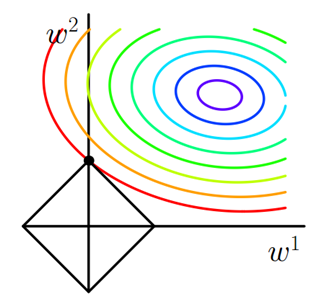
\includegraphics[width = 0.7\textwidth]{figures_ning/l1.png}
	\caption[The architecture of Faster R-CNN]
	{ L1 Regularization.}
	\label{fig:l1}
\end{figure}

The contour in the figure above is the contour of $J_{0}$ and the black square is the graph of the $L$ function. In the figure, the optimal solution is found when the $J_{0}$ contour intersects the graph of $L$ for the first time. In the above graph $J_{0}$ and $L$ intersect at a vertex of $L$. This vertex is the optimal solution. Notice that the value of this vertex is $\left(w_{1}, w_{2}\right)=\left(0, w_{2}\right)$. It can be intuitively imagined that because the $L$ function has many prominent corners (four in the two-dimensional case and more in the multidimensional case), the chance of $J_{0}$ coming into contact with these corners will be much greater than the chance of coming into contact with the rest of $L$. At these corners, there will be many weights equal to zero, which is why $L_{1} regularization$ can produce a sparse model, which in turn can be used for feature selection.

The coefficient $\lambda$ in front of the regularization can control the size of the graph of $L$. The smaller $\lambda$ is, the larger the graph of $L$ (the black box in the above figure); the larger $\lambda$ is, the smaller the graph of $L$ can be so small that the black box is only a little beyond the origin range, which is the most advantageous value  $\left(w_{1}, w_{2}\right)=\left(0, w_{2}\right)$ in which $w_{2}$ can be taken to a very small value.

Similarly, and $L_{2}$ regularized loss function: $J=J_{0}+\lambda \sum_{w} w^{2}$,the same can be drawn its image in the two-dimensional plane as follows:
\begin{figure}[!htbp]
	\centering
	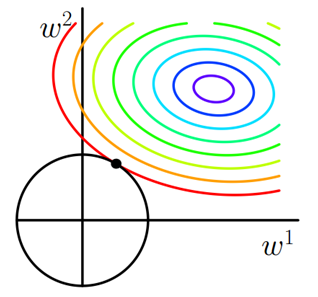
\includegraphics[width = 0.7\textwidth]{figures_ning/l2.png}
	\caption[L2 Regularization]
	{ L2 Regularization.}
	\label{fig:l2}
\end{figure}

The graph of the $L_{2}-regularized$ function in the two-dimensional plane is a circle, which is ground away from the corners compared to a square. Therefore the chance of making $w_{1}$ or $w_{2}$ equal to zero when $J_{0}$ intersects $L$ is much smaller, which is why the $L_{2}-regularization$ is not sparse

\subsection{$\ell 1-n o r m$ Prevents Overfitting}

The fitting process usually tends to make the weights as small as possible and finally construct a model with all parameters relatively small. This is because it is generally believed that models with small parameter values are simpler, can be adapted to different data sets, and also avoid the overfitting phenomenon to some extent. For a linear regression equation, if the parameters are large, then as long as the data is shifted a little, it will have a great impact on the results; but if the parameters are small enough, a little more data shift will not have any impact on the results, that is, it is highly resistant to perturbation.

Take the gradient descent method in linear regression as an example. Assuming that the required parameter is $\theta$ and  $h \theta(x)$ is our assumed function, the cost function of linear regression is as follows:
$$
J_{\theta}=\frac{1}{2 n} \sum_{i=1}^{n}\left(h \theta\left(x^{(i)}\right)-y^{(i)}\right)^{2}
$$
The iterative formula for $\theta$ in gradient descent is:
$$
\theta_{j}=\theta_{j}-\alpha \frac{1}{n} \sum_{i=1}^{n}\left(h \theta\left(x^{(i)}\right)-y^{(i)}\right) x_{j}^{(i)}
$$

where $\alpha$ is the learning rate. The above equation is the iterative formula without adding the $L_{2}$ regularization term. If $L_{2}$ regularization is added after the original cost function, the iterative formula is:
$$
\theta_{j}=\theta_{j}\left(1-\alpha \frac{\lambda}{n}\right)-\alpha \frac{1}{n} \sum_{i=1}^{n}\left(h \theta\left(x^{(i)}\right)-y^{(i)}\right) x_{j}^{(i)}
$$

where $\lambda$ is the regularization parameter. As can be seen from the above equation, compared to the iterative formula without adding $L2 regularization$, at each iteration, $\theta_{j}$ is first multiplied by a factor less than 1, which makes $\theta_{j}$ decreasing, so in total, $\theta$ is decreasing.Therefore $L2$ regularization can obtain smaller parameters and thus prevent overfitting.

\section{Signal Processing}

The first step of machine learning is to extract the corresponding features. If the input data is a picture, for example, a 28*28 picture, then only each pixel needs to be used as a feature, and the corresponding pixel value size (representing the intensity of the color) can be used as the feature value. Then in the field of audio and speech signal processing, we need to convert the signal into a corresponding speech spectrogram, and use the data on the speech spectrogram as the features of the signal. The horizontal axis $x$ of the spectrogram is time, the vertical axis $y$ is frequency, and the value corresponding to $(\mathrm{x}, \mathrm{y})$ represents the amplitude of frequency $y$ at time $x$. However, the human ear is logarithmic in its perception of frequency, i.e., sensitive to changes in the lower frequency bands and sluggish to changes in the higher frequency bands, so a linearly distributed speech spectrogram is obviously "not useful enough" for feature extraction, so the Meier speech spectrogram Therefore, the Meier spectrum map was created. The vertical frequency and the original frequency of Meier's speech spectrogram are interchanged by the following formula:
$$
\begin{gathered}
	m=2595 \log _{10}\left(1+\frac{f}{700}\right) \\
	f=700\left(10^{m / 2595}-1\right)
\end{gathered}
$$

$f$ represents the original frequency and $m$ represents the transformed Mel frequency. Obviously, when $f$ is large, the change of m tends to be flat. And the Meier cepstrum coefficients (MFCCs) are obtained by cosine transformation (DCT, a linear transformation similar to the Fourier transform) and then taking some of the coefficients.
The Melody score chart is divided into the following steps. An audio file is used as an example to show the principle of each step.

\subsection{Get Audio Signal}

python can use the librosa library to read audio files, but for MP3 files, it will automatically call the audio read function, so if it is an MP3 file, make sure to add the path to ffmpeg.exe to the system environment variable, otherwise the audio read function will error out. Here we first read the audio file and make a waveform from 0-20 seconds. Nowadays, the sampling rate of music files is usually 44.1 kHz. 
\begin{figure}[!htbp]
	\centering
	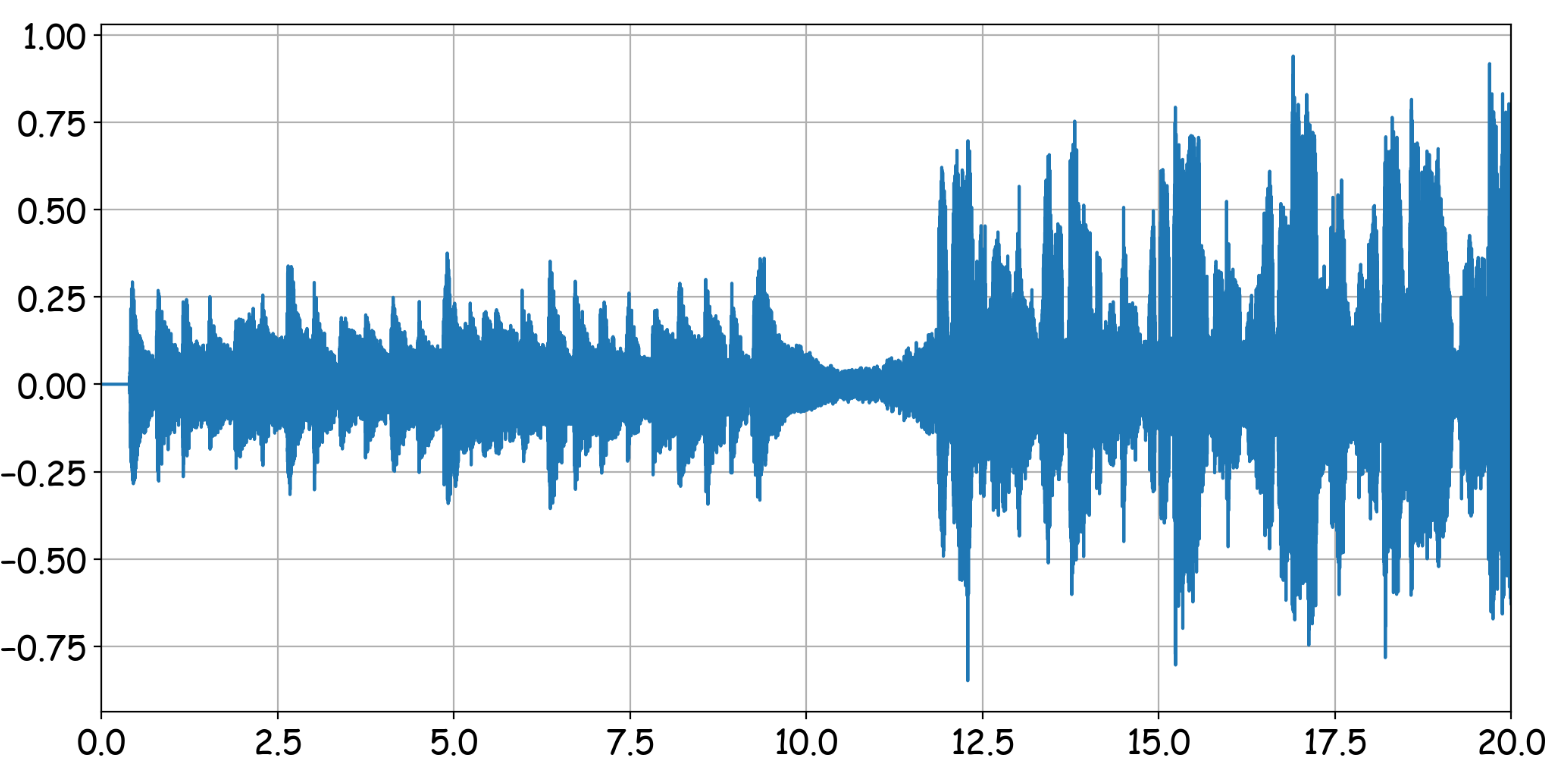
\includegraphics[width = 0.7\textwidth]{figures_ning/audio_1.png}
	\caption[L2 Regularization]
	{ Amplitude of audio signal.}
	\label{fig:audio_1}
\end{figure}

\subsection{Pre-Emphasis}

Generally speaking, the high-frequency component of the speech/audio signal has a small strength and the low-frequency component has a large strength. Signal pre-emphasis is to let the signal pass through a high-pass filter so that the strengths of the high and low frequency components of the signal do not differ too much. In the time domain, the signal $x[n]$ is operated as follows:
$$
y[n]=x[n]-\alpha x[n-1]
$$

$\alpha$ is usually taken as a value very close to 1, with a typical value of 0.97 or 0.95. From the time domain formula, some people may not understand why this is a high-pass filter, so let's look at the transfer function of the filter from the perspective of z-transform:
$$
H(z)=\frac{Y(z)}{X(z)}=1-\alpha z^{-1}=\frac{z-\alpha}{z}
$$

It can be seen that the filter has a pole 0 and a zero point $\alpha$. When the frequency is 0, z=1, the amplification factor is $(1-\alpha)$. As the frequency increases, the amplification factor becomes larger, and when the frequency reaches $p_{i}$, the amplification factor is $(1+ \alpha)$. In the discrete domain, $[0, p_{i}]$ corresponds to $[0, \mathrm{fs} / 2]$ in the continuous domain (in Hz). Where fs is the sampling rate, which in our case is 44.1 kHz. so the amplification factor is $(1+ \alpha)$ when the frequency goes to 22000 Hz. The following figure shows the generated graph:
\begin{figure}[!htbp]
	\centering
	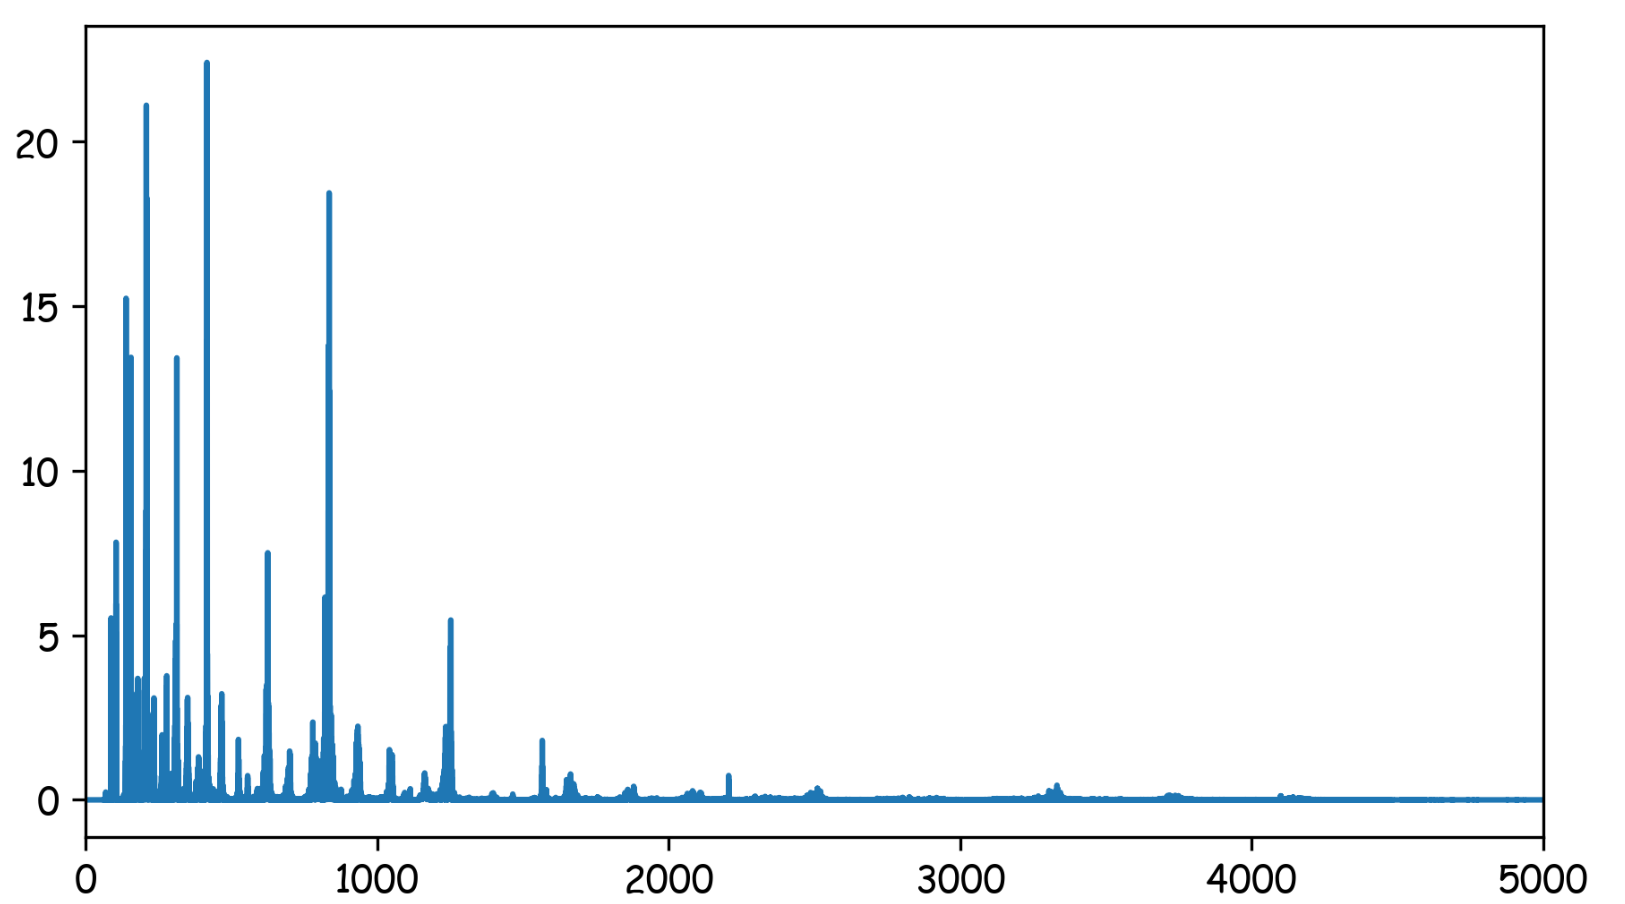
\includegraphics[width = 0.7\textwidth]{figures_ning/audio_2.png}
	\caption[Unpre-emphasized signal spectrum]
	{ Unpre-emphasized signal spectrum}
	\label{fig:audio_2}
\end{figure}

\begin{figure}[!htbp]
	\centering
	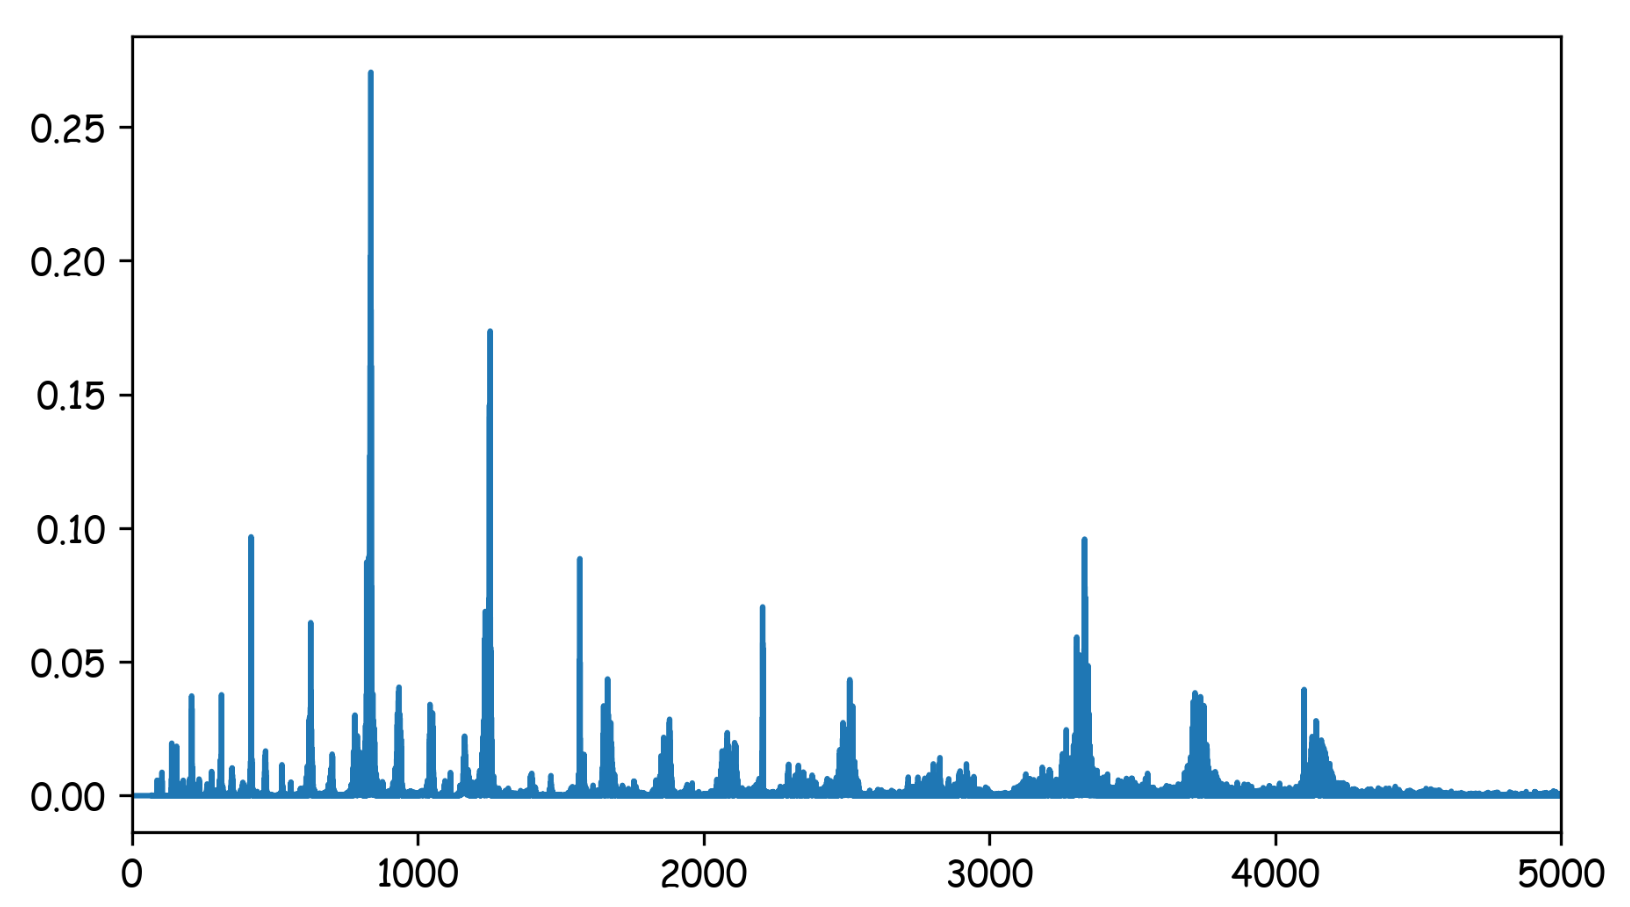
\includegraphics[width = 0.7\textwidth]{figures_ning/audio_3.png}
	\caption[Pre-emphasized signal spectrum]
	{ Pre-emphasized signal spectrum}
	\label{fig:audio_3}
\end{figure}

The code of both graphs uses the function librosa.fft.rfft(y,n), $rfft$ means that after the FFT transform only half of it is taken (because the other half corresponds to negative frequencies, which are useless), $y$ corresponds to the signal, and $n$ corresponds to the number of points to do the FFT. The actual frequency corresponding to each point is the index value of the point ${ }^{*} \mathrm{f_{s}} / \mathrm{n}$. How is this obtained? Because the 882,000th point should correspond to (approximately equal to) $f_{s}$ (or 2$p_{i}$ in the discrete domain), so the previous points can correspond one by one according to the linear relationship. Only 0-5000Hz is shown here, and it can be seen that the difference between the high-frequency component of the signal after pre-emphasis and the low-frequency component is obviously not so big.
The result of pre-emphasis:
\begin{enumerate}[\qquad  1.]
	\item Balance between high and low frequencies.
	\item Avoid numerical problems in the FFT (i.e., high frequency values that appear too small in the denominator may go wrong).
	\item Possible improvement of SNR.
\end{enumerate}

\subsection{Framing}

The time covered by the original signal is too long, and using it as a whole to do FFT, we can only get the relationship between signal frequency and intensity, and lose the time information. Therefore, after pre-processing the signal, the original signal should be divided into several small pieces according to time, and one piece is called a frame. We want to get the relationship between frequency and time, so we divide the original signal into several frames, make FFT for each frame (also called short-time FFT, because we only take a small period of time), and then stitch the obtained results together in time order. This is the principle of spectrogram.
Several variables are defined below:
\begin{itemize}
	\item \textbf{Frame Size:} Length of each frame. Usually it is 20-40ms, too long will result in a small time resolution, too small will increase the computational cost. Here we take 25ms.
	\item \textbf{Frame Length:} The number of samples per frame. This is equal to ${ }^{*} f_{s}*frame_size$, which is 44.1k*0.025=1102.
	\item \textbf{Frame Stride:} The interval between two adjacent frames. Usually the interval must be less than the length of each frame, i.e. there should be an overlap between the two frames, otherwise the information near the boundary of the two frames may be removed. When doing feature extraction, it is never desirable to remove the useful information. Here we take 10ms, i.e. there is $60 \%$overlap.
	\item \textbf{Frame Step:} The number of samples in two adjacent frames. Here is 441.
	\item \textbf{Frame Num:} The number of frames needed for the entire signal. The number of frames needed is generally expected to be an integer value, so the signal should be zero padded so that the length of the signal can be divided into integer frames.
\end{itemize}

\subsection{Window}

After splitting the frames, a window function is added to each frame to get a better sidelobes. Usually a hamming window is used.

In this process of frame splitting, it is equivalent to adding a rectangular window to the signal, the spectrum of the rectangular window has a large sidelobes, and the window function is multiplied with the original function in the time domain, which is equivalent to the convolution in the frequency domain. This is the spectral leakage.

\subsection{Power Spectrum}

Since each line is a 1102-point signal, we can choose a 1024-point FFT (fewer FFT points than the original signal will reduce the frequency resolution, but the difference here is small, so we can (ignore). The power spectrum is obtained by taking the magnitude of the obtained FFT transform and dividing it by the corresponding number of FFT points. At this point we have actually obtained the spectrogram, we just need to use plt.imshow to draw the heat map corresponding to its dB value.
\begin{figure}[!htbp]
	\centering
	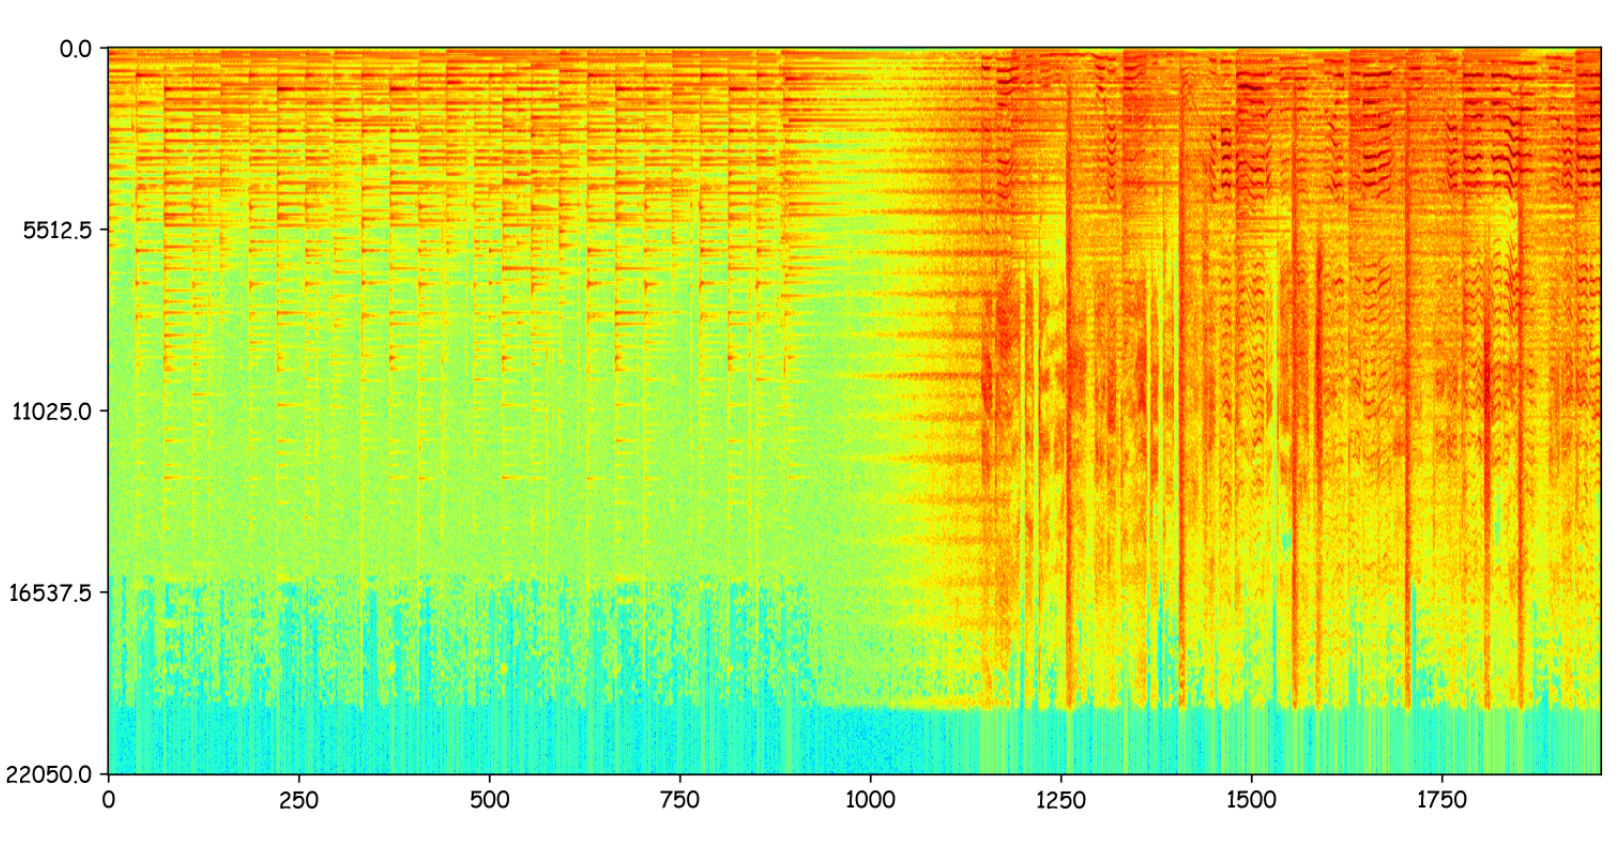
\includegraphics[width = 0.7\textwidth]{figures_ning/audio_4.png}
	\caption[Heat Map]
	{ Heat Map}
	\label{fig:audio_4}
\end{figure}

\subsection{Mel-filter Banks}

The last step is to apply the Mel filter to the pow-frames obtained in the previous step. The so-called Mayer filter bank is a triangular filter bank of equal height, where each filter starts at the midpoint of the previous filter. The corresponding frequencies are linear on the Meier scale, hence the name Meier filter bank. The frequency corresponding to each filter can be converted from the maximum frequency (4000 in the figure below, 22.05k in our case) to the Mel frequency using the formula mentioned above, divided linearly into several frequency bands on the Mel scale, and then converted back to the actual frequency scale. In practice, each filter is dotted with the power spectrum pow-frames and the result is the energy in the band. Here our pow-frames is a (1999,513) matrix, Mel filter fbank is a (mel-N, 513) matrix, where mel-N represents the number of corresponding Mel filters, this value can not be too large, because here we only have a total of 513 points, if mel-N is too large, will lead to the length of the first few filters are If mel-N is too large, the length of the previous filters will be 0 (because the low-frequency mel filters are particularly narrow). T can be obtained by multiplying these two matrices by pow-frames*F-bank.T. The result is a (1999, 40) matrix, where each row is a frame and each column represents the energy of the corresponding mel band. An example of a specific mel filter is shown below:
\begin{figure}[!htbp]
	\centering
	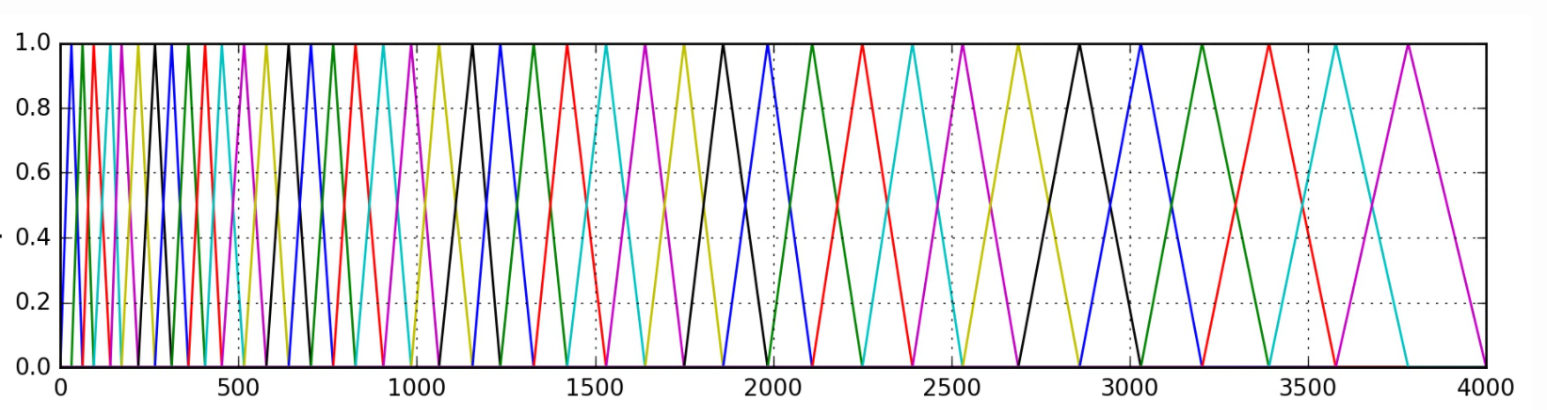
\includegraphics[width = 0.7\textwidth]{figures_ning/audio_5.png}
	\caption[Filter bank on a Mel-scale]
	{ Filter bank on a Mel-scale}
	\label{fig:audio_5}
\end{figure}

\subsection{Mel-spectogram Feature}

In machine learning, each audio segment can be represented by a corresponding mel-spectogram, and each frame corresponding to a certain frequency band is a feature. In practice, each audio has to be of the same length so that we have the same number of features. Usually, normalization is also performed, i.e., each element of each frame is subtracted from the average value of that frame to ensure that the average value of each frame is 0. Finally, the Mel-spectrogram is obtained as follows:

\begin{figure}[!htbp]
	\centering
	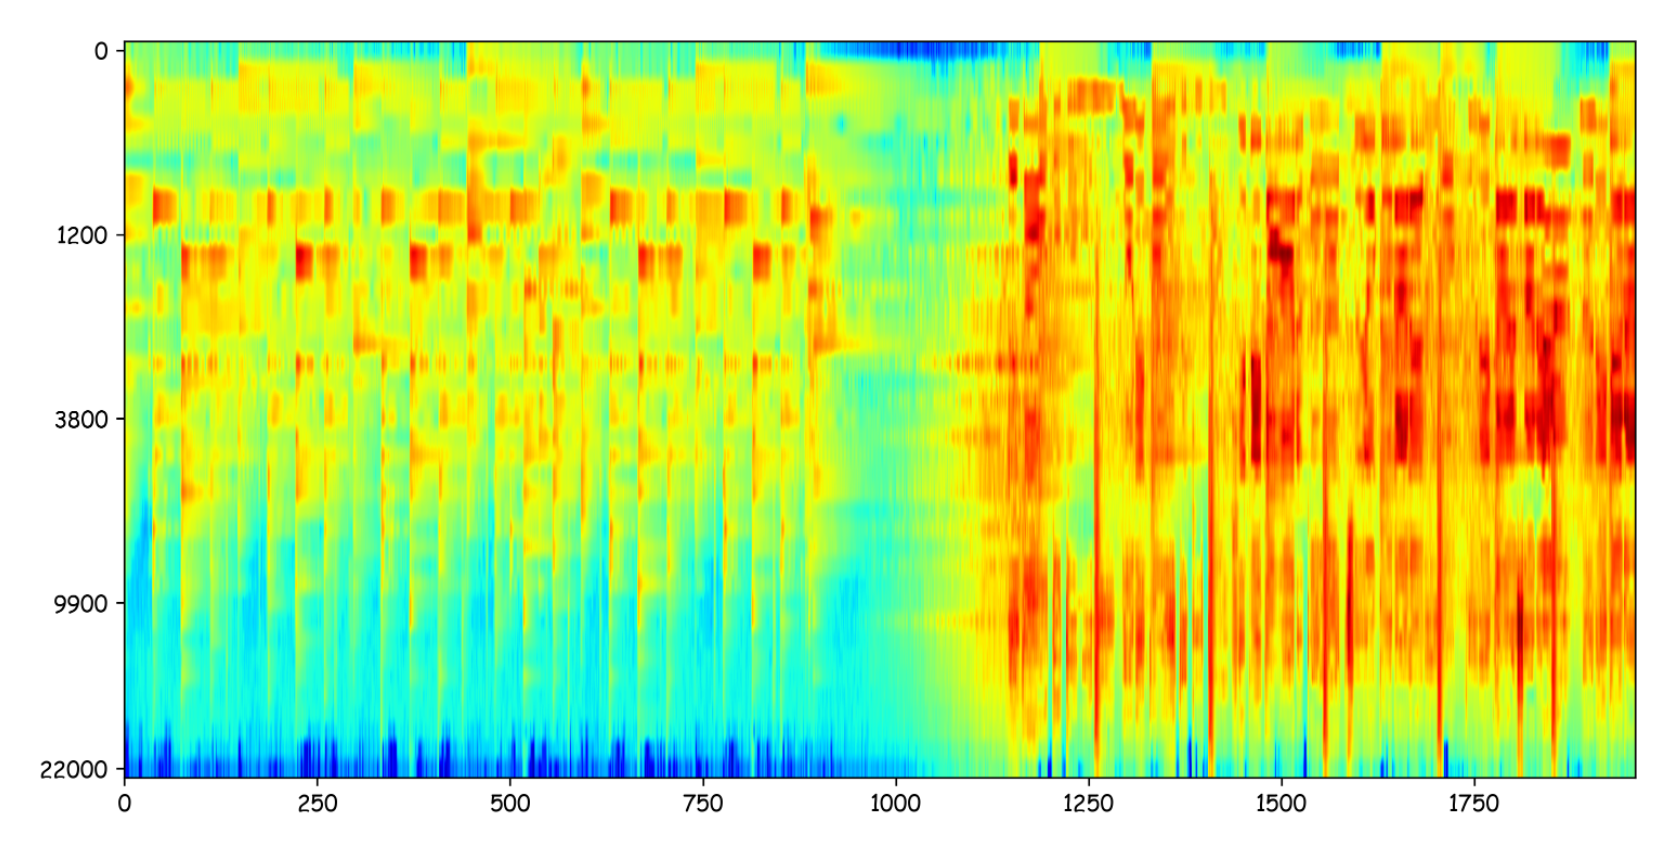
\includegraphics[width = 0.7\textwidth]{figures_ning/audio_6.png}
	\caption[Mel-spectogram]
	{ Mel-spectogram}
	\label{fig:audio_6}
\end{figure}

\subsection{VGG16}

VGG16 is a convolutional neural network model proposed by K. Simonyan and A. Zisserman from the University of Oxford in the paper ``Very Deep Convolutional Networks for Large-Scale Image Recognition''~\cite{simonyan2015deep}. The model achieves 92.7\% top-5 test accuracy in ImageNet~\cite{ILSVRC15}, which is a dataset of over 14 million images belonging to 1000 classes.

The structure of VGG16 is shown in Fig.~\ref{fig:vgg16}.The input to cov1 layer is of fixed size 224 x 224 RGB image. The image is passed through a stack of convolutional (conv.) layers, where the filters were used with a very small receptive field: 3x3 (which is the smallest size to capture the notion of left/right, up/down, center). In one of the configurations, it also utilizes 1x1 convolution filters, which can be seen as a linear transformation of the input channels (followed by non-linearity). The convolution stride is fixed to 1 pixel; the spatial padding of conv. layer input is such that the spatial resolution is preserved after convolution, i.e. the padding is 1-pixel for 3x3 conv. layers. Spatial pooling is carried out by five max-pooling layers, which follow some of the conv.  layers (not all the conv. layers are followed by max-pooling). Max-pooling is performed over a 2x2 pixel window, with stride 2.

Three Fully-Connected (FC) layers follow a stack of convolutional layers (which has a different depth in different architectures): the first two have 4096 channels each, the third performs 1000-way ILSVRC classification and thus contains 1000 channels (one for each class). The final layer is the soft-max layer. The configuration of the fully connected layers is the same in all networks.

All hidden layers are equipped with the rectification (ReLU) non-linearity. It is also noted that none of the networks (except for one) contain Local Response Normalisation (LRN), such normalization does not improve the performance on the ILSVRC dataset, but leads to increased memory consumption and computation time.


\begin{figure}[!htbp]
	\centering
	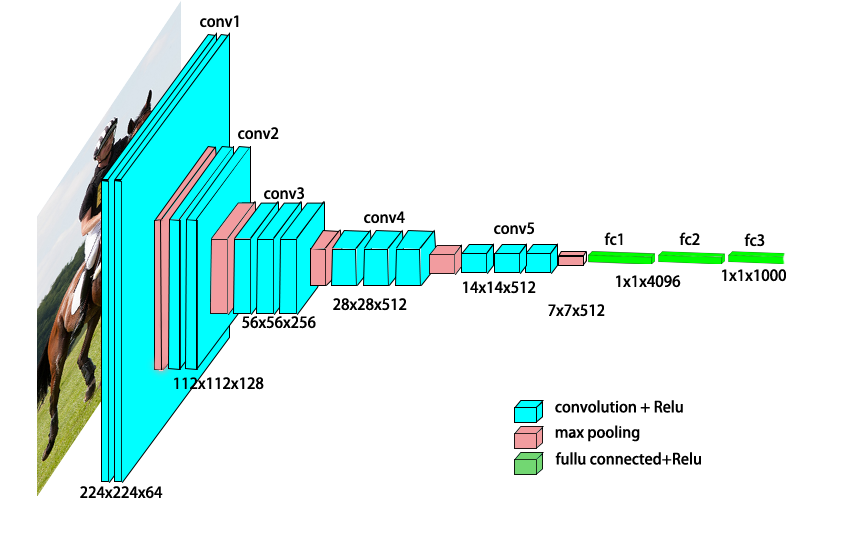
\includegraphics[width=0.8\linewidth]{figures/vgg16}
	\caption[The Architecture of VGG-16]{The Architecture of VGG-16.}
	\label{fig:vgg16}
\end{figure}

The advantages of VGG:
\begin{itemize}
	\item The structure of VGGNet is very simple, the entire network uses the same size of the convolution kernel size (3x3) and maximum pooling size (2x2).
	\item The combination of several small filter (3x3) convolutional layers is better than a large filter (5x5 or 7x7) convolutional layer.
	\item It is verified that performance can be improved by continuously deepening the network structure.
\end{itemize}

The disadvantages of VGG:

\begin{itemize}
	\item VGG consumes more computing resources and uses more parameters, resulting in more memory usage. Most of the parameters are from the first fully connected layer. VGG has 3 fully connected layers.
\end{itemize}




\chapter{Methodology}
\label{chap:framework}
First, we introduce in this chapter a lifelong learning approach for Dynamic Neural Networks~\cite{yoon2017lifelong}, which is a way to achieve simultaneous and effective multitasking by dynamically extending the neural network structure. Then our proposed framework based on the DEN model is described in detail.


\section{Related Work}\label{sec:related-4}

Lifetime learning, i.e., the problem of continuous learning where tasks arrive sequentially, is an important topic in transfer learning. The main goal of lifelong learning is to exploit the knowledge from earlier tasks to obtain better performance or to obtain faster convergence/training speed on the model for later tasks, but without forgetting the previous knowledge, i.e., the model parameters apply to the previous model.

Regarding lifelong learning, there are also many different approaches to implementation. The simplest approach is to gradually fine-tune the network to fit the new task by continuing to train the network with new training data. However, this simple retraining of the network can degrade the performance of both the new task and the old task. If the new task is very different from the old task, then the model trained for the new task, changes so much that it is no longer applicable to the old task. For example, the lifelong learning approach using  Elastic Weight Consoliation(EWC)~\cite{kirkpatrick2017overcoming} is as follows:
\begin{figure}[H]
	\centering
	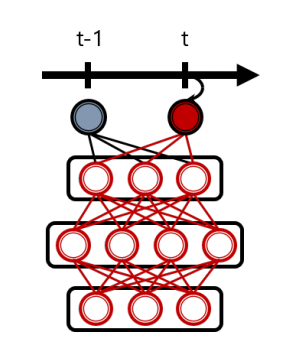
\includegraphics[width=1\linewidth]{figures_ning/ewc}
	\caption[Retraining w/o expansion]{Retraining w/o expansion}
	\label{fig:ewc}
\end{figure}
Elastic Weight Consoliation retrains the entire network learned in the previous task, while regularizing it to prevent large deviations from the original model. Units and weights in red indicate retrained units and weights, while black indicates units and weights that remain fixed.

The use of the EWC approach, i.e., limiting the weights, leads to smaller changes in the parameters, thus allowing the model trained for the new task to also be valid for the old task at the same time.

Of course, the disadvantage of this approach is also obvious. When the difference between the old and new tasks is large, it is difficult to make the model valid for the new task no matter how it is trained, because the elasticity limits the model parameters.

In addition to this there is a lifelong learning approach, fixed extension neural networks~\cite{rusu2016progressive}. For a new task, the original model parameters are no longer retrained, and a fixed number of neurons are directly expanded on the original neural network structure. In the subsequent training, only the newly added neurons are trained, and no further changes are made to the previous model parameters.
\begin{figure}[H]
	\centering
	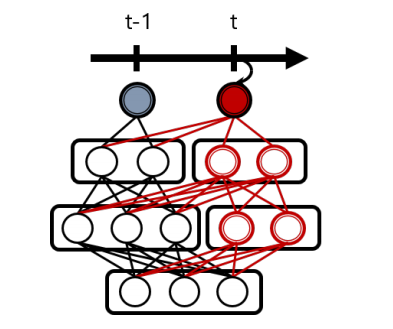
\includegraphics[width=1\linewidth]{figures_ning/no-train}
	\caption[No-retraining w/ expansion]{No-retraining w/ expansion}
	\label{fig:no-train}
\end{figure}
Units and weights colored in red denote the ones that are retrained, and black ones are ones that remain
fixed.

The disadvantage of this approach is also obvious, it is difficult to have an effect on the new task by the newly added part of neurons, because there are too few parameters that can be changed, or the previous parameters are too important.

However for such incremental deep learning setups with selective parameter sharing and dynamic layer scaling, many challenges need to be addressed.
\begin{enumerate}[\qquad  1.]
	\item Achieving scalability and efficiency in training: If the network capacity grows, the training cost per task will also get higher, as later tasks will establish connections to larger networks. Therefore, we need a way to keep the computational overhead of retraining low.
	\item Decide when to scale the network and how many neurons to add: If the old network adequately explains the new task, the network may not need to scale its size. On the other hand, if the task is very different from the existing one, it may need to add many neurons. Therefore, the model needs to dynamically add only the necessary number of neurons.
	\item prevent semantic drift or catastrophic forgetting, where the network deviates from its initial configuration during training, thus showing degraded performance of earlier examples/tasks. Since our approach retrains the network, even partially, to adapt to later learned tasks and adds new neurons that may also negatively affect previous tasks by establishing connections to older sub-networks, we need a mechanism to prevent potential semantic drift.
\end{enumerate}

To overcome these challenges, we propose a novel deep network model and an efficient and effective incremental learning algorithm, which we name as Dynamically Extensible Network (DEN). In a lifelong learning scenario, DEN maximizes the network learned on all previous tasks to efficiently learn to predict new tasks, while dynamically increasing the network capacity by adding or splitting neurons when necessary.

DEN solves the challenge presented above very well, since we retrain the network on each task t so that each new task only utilizes and changes relevant parts of the previously trained network, while still allowing to extend the network capacity if necessary. In this way, each task t will use a different sub-network from the previous task while still sharing a significant portion of the sub-network with them. As shown in the figure below:
\begin{figure}[H]
	\centering
	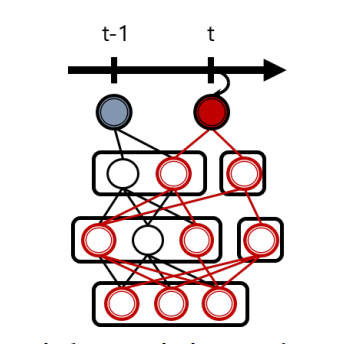
\includegraphics[width=1\linewidth]{figures_ning/den}
	\caption[Partial retraining w/ expansion]{Partial retraining w/ expansion}
	\label{fig:den}
\end{figure}

The advantages of the DEN method are also obvious, as more parameters can be changed to better suit the new task, while not forgetting the parameters of the old task.

\section{Dynamic Neural Networks}

We consider the problem of incremental training of deep neural networks in a lifelong learning scenario, where the unknown number of tasks with unknown distribution of training data arrive sequentially to the model. Specifically, we aim to learn a model for a series of $T$ tasks, $t = 1, . . . , t, . . . , T$ denotes unbounded $T$ where the task at time point $t$ comes with training data $\mathcal{D}_{t}=\left\{\boldsymbol{x}_{i}, y_{i}\right\}_{i=1}^{N_{t}}$. Note that each task $t$ can be a single task or can consist of a set of subtasks.
This approach is general for any type of task. In this experiment, what we need to do is to attack the defense model by adding interference terms to the original data and turning it into fake data. Briefly, we are binary classification task, i.e. $y \in\{0,1\}$ for input features $\boldsymbol{x} \in \mathbb{R}^{d}$. The main challenge in the lifetime learning setup is that all previous training datasets up to $t-1$ are not available at the current time $t$ (only the model parameters of the previous task are accessible, if any). The lifelong learning agent at time t aims to learn the model parameters $\boldsymbol{W}^{t}$ by solving the following problems:
$$
\underset{\boldsymbol{W}^{t}}{\operatorname{minimize}} \mathcal{L}\left(\boldsymbol{W}^{t} ; \boldsymbol{W}^{t-1}, \mathcal{D}_{t}\right)+\lambda \Omega\left(\boldsymbol{W}^{t}\right), \quad t=1, \ldots
\label{eq:1}
$$

where $\mathcal{L}$ is the task-specific loss function, $\boldsymbol{W}^{t}$ is the parameter of task $t$, and $\Omega\left(\boldsymbol{W}^{t}\right)$ is the regularization (e.g., elemental $\ell_{2}$ norm parametrization) to properly execute our model $\boldsymbol{W}^{t}$. For our main neural network of interest, $\boldsymbol{W}^{t}=\left\{\boldsymbol{W}_{l}\right\}_{l=1}^{L}$ is the weight tensor.

\begin{figure}[H]
	\centering
	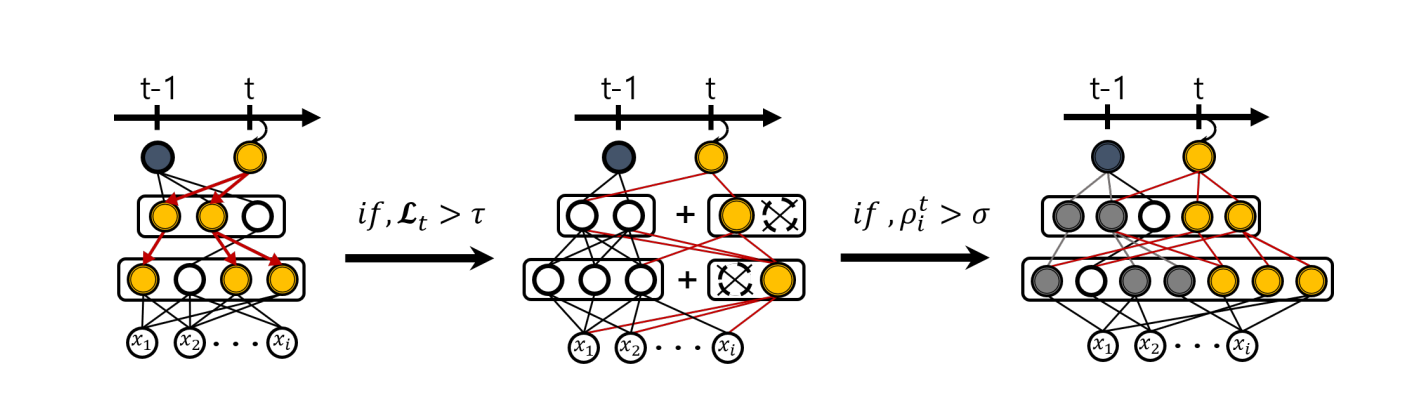
\includegraphics[width=1\linewidth]{figures_ning/den-real}
	\caption[selcted]{expension}
	\label{fig:den-real}
\end{figure}
To address these challenges of lifelong learning, we allow the network to maximize the knowledge gained from previous tasks, while allowing it to dynamically expand its capacity when the accumulated knowledge alone does not adequately explain new tasks. Figure~\ref{fig:den-real} and Algorithm 1 depict our incremental learning process.
\begin{algorithm}[ht]
	\caption{Incremental Learning of a Dynamically Expandable Network}  
	\begin{algorithmic}[1]
		\Require Dataset $\mathcal{D} = (\mathcal{D}_1, \ldots , \mathcal{D}_T )$, Thresholds $\tau,\sigma$
		\Ensure $\bm{W}^T$
		\For{$t=1,\ldots,T$}
		\If{t=1}
		\State Train the network weights $\bm{W}^1$ using Eq.\ref{eq:2}
		\Else
		\State $\bm{W}^t = SelectiveRetraining(\bm{W}^{t-1})$\{Selectively retrain the previous network using Algorithm2\}
		\If{$\mathcal{L}_t>\tau$}
		\State $\bm{W}^t = DynamicExpansion(\bm{W}^{t})$ \{Expand the network capacity using Algorithm3\}
		\EndIf
		\State $\bm{W}^t = Split(\bm{W}^t)$ \{Split and Initialize the units using Algorithm4\}
		\EndIf
		\EndFor
	\end{algorithmic} 
\end{algorithm}

After referring to the research results of others~\cite{yoon2017lifelong}, it was considered that changes should be made in the last step, which is the third step of the algorithm. If the final trained model parameters, i.e., $W$, change relatively large, resulting in the newly trained model no longer being applicable to the old task, they believe that the original nodes should be copied and then retrained~\cite{yoon2017lifelong}. In our experiments, a new approach is taken, where if the model parameters change relatively large, the parameters with large changes are initialized directly after all training is completed, which can satisfy that the newly trained model works well for both the old and new tasks.

In the following subsections, we describe in detail each component of the incremental learning algorithm: 
\begin{itemize}
	\item Selective Retraining
	\item Dynamic Network Expansion
	\item Network Splitting and Initializing
\end{itemize}

\subsection{Selective Retraining}
The easiest way to train a model for a series of tasks is to retrain the entire model each time a new task arrives. However, such retraining would be very expensive for deep neural networks. Therefore, we propose to selectively retrain the model by retraining only the weights affected by the new task. Initially ($t$ = 1), we train the network with $\ell 1$-regularization to promote sparsity of weights so that each neuron is connected to only a few neurons in the following layers:
$$
\underset{\boldsymbol{W}^{t=1}}{\operatorname{minimize}} \mathcal{L}\left(\boldsymbol{W}^{t=1} ; \mathcal{D}_{t}\right)+\mu \sum_{l=1}^{L}\left\|\boldsymbol{W}_{l}^{t=1}\right\|_{1}
\label{eq:2}
$$

Such retraining would be very expensive for deep neural networks. Therefore, we propose to selectively retrain the model by retraining only the weights affected by the new task. Initially (t=1), we train the network with l1-regularization to promote sparsity of the weights so that each neuron is connected to only a few neurons in the following layers.

where $1 \leq l \leq L$ denotes the lth layer of the network, $\boldsymbol{W}_{l}^{t}$ is the network parameter of the lth layer, and $\mu$ is the regularization parameter of the element-wise l1-parametrization of sparsity on $W$ . For the convolutional layer, we apply (2 , 1)-norm on the filters and select only a few filters from the previous layer.
During our incremental learning process, we keep $\boldsymbol{W}^{t-1}$ sparse, so we can significantly reduce the computational overhead if we can focus on new tasks connected to the subnetwork. To this end, when a new task t arrives at the model, we first fit a sparse linear model that predicts the task t using the highest hidden unit of the neural network by solving the following problem:
$$
\underset{\boldsymbol{W}_{L, t}^{t}}{\operatorname{minimize}} \mathcal{L}\left(\boldsymbol{W}_{L, t}^{t} ; \boldsymbol{W}_{1: L-1}^{t-1}, \mathcal{D}_{t}\right)+\mu\left\|\boldsymbol{W}_{L, t}^{t}\right\|_{1}
\label{eq:3}
$$
where $\boldsymbol{W}_{1: L-1}^{t-1}$ denotes the set of all other parameters except $\boldsymbol{W}_{L, t}^{t}$. That is, we solve this optimization to obtain a connection between the output unit ot and the hidden unit in the $L$-1 layer (fixing all other parameters to the $L$-1 layer as $\boldsymbol{W}^{t-1}$). Once we have established sparse connections at this layer, we can identify all the units and weights in the network that are affected by the training, while keeping the parts of the network that are not connected to $o_t$ unchanged. Specifically, we perform a breadth-first search on the network starting from those selected nodes to identify all units (and input features) that have a path to ot. Then, we train only the weights of the selected subnetwork S, denoted as $\boldsymbol{W}_{S}^{t}$:
$$
\underset{\boldsymbol{W}_{S}^{t}}{\operatorname{minimize}} \mathcal{L}\left(\boldsymbol{W}_{S}^{t} ; \boldsymbol{W}_{S^{c}}^{t-1}, \mathcal{D}_{t}\right)+\mu\left\|\boldsymbol{W}_{S}^{t}\right\|_{2}
\label{eq:4}
$$

We use element-by-element $\ell_{2}$-regularizers because sparse connections have already been established. This partial retraining will result in a lower computational overhead and also help to avoid negative migration, since unselected neurons will not be affected by the retraining process. Algorithm~\ref{algorithm:2} describes the selective retraining process:

\begin{algorithm}[ht]
	\caption{Selective Retraining}  
	\begin{algorithmic}[1]
		\Require Dataset $\mathcal{D}_t$, Previous parameter $\bm{W}^{t-1}$
		\Ensure network parameter $\bm{W}^t$
		\State Initialize $l\leftarrow L-1$, $S=\{o_t\}$
		\State Solve Eq.~\ref{eq:3} to obtain $\bm{W}^t_{L,t}$
		\State Add neuron $i$ to $S$ if the weight between $i$ and $o_t$ in $\bm{W}^t_{L,t}$ is not zero.
		\For{$l=L-1,\ldots,1$}
		\State Add neuron $i$ to $S$ if there exists some neuron $j \in S$ such that $\bm{W}^{t-1}_{l,ij}\neq 0$.
		\EndFor
		\State Solve Eq.~\ref{eq:4} to obtain $\bm{W}^t_{S}$
	\end{algorithmic}
	\label{algorithm:2} 
\end{algorithm}

\subsection{Dynamic Network Expansion}
Selective retraining alone is sufficient for the new task if it is highly relevant to the old task or if the aggregated partial knowledge gained from each task is sufficient to explain the new task. However, when the learned features do not accurately represent the new task, additional neurons need to be introduced into the network to take into account the features required for the new task. Some existing works~\cite{rusu2016progressive}are based on a similar idea. However, they are either inefficient due to the need to repeat the iterative training of the forward pass~\cite{zhou2012online} or add a constant number of units in each task t without considering the task difficulty~\cite{rusu2016progressive} and thus are not optimal in terms of performance and network capacity utility.
To overcome these limitations, we propose an efficient approach that uses group sparse regularization to dynamically decide how many neurons to add at which layer for each task without repeatedly retraining the network for each unit. Suppose we extend the $l_{th}$ layer of the network with a constant number of units, say $k$, and introduce two parameter matrix extensions: $\boldsymbol{W}_{l}^{t}=\left[\boldsymbol{W}_{l}^{t-1} ; \boldsymbol{W}_{l}^{\mathcal{N}}\right]$ and $\boldsymbol{W}_{l-1}^{t}=\left[\boldsymbol{W}_{l-1}^{t-1} ; \boldsymbol{W}_{l-1}^{\mathcal{N}}\right]$ for the efferent and afferent layers, where $W^{\mathcal{N}}$ is the extended weight matrix associated with the added neurons. Since we do not always want to add all $k$ units (depending on the correlation between the new and old tasks), we perform group sparse regularization of the added parameters as follows:
$$
\underset{\boldsymbol{W}_{l}^{\mathcal{N}}}{\operatorname{minimize}} \mathcal{L}\left(\boldsymbol{W}_{l}^{\mathcal{N}} ; \boldsymbol{W}_{l}^{t-1}, \mathcal{D}_{t}\right)+\mu\left\|\boldsymbol{W}_{l}^{\mathcal{N}}\right\|_{1}+\gamma \sum_{g}\left\|\boldsymbol{W}_{l, g}^{\mathcal{N}}\right\|_{2}
\label{eq:5}
$$

where $g \in \mathcal{G}$ is the group defined over the incoming weights of each neuron. For the convolutional layer, we define each group as the activation map of each convolutional filter. This group sparse regularization was used by~\cite{wen2016learning} and ~\cite{alvarez2016learning} to find the correct number of neurons for the complete network, while we apply it to parts of the network. Algorithm~\ref{algorithm:3} describes the details of how the extension works.
After selective retraining is completed, the network checks if the loss is below a certain threshold. If not, then at each layer we expand its capacity by $k$ neurons and solve the Eq~\ref{eq:5}. Due to the sparse regularization of the set of Eq.~\cite{eq:5}, the hidden units (or convolutional filters) that are considered unnecessary in the training will be removed completely. We expect that from this dynamic network expansion process, the model captures new features not previously represented by$\boldsymbol{W}_{l}^{t-1}$ to minimize residuals while maximizing the network capacity by avoiding adding too many units.

\begin{algorithm}[h!]
	\caption{Dynamic Network Expansion}  
	\begin{algorithmic}[1]
		\Require Dataset $\mathcal{D}_t$, Threshold $\tau$
		\State Perform Algorithm \ref{label} and compute $\mathcal{L}$
		\If{$\mathcal{L}>\tau$}
		\State Add $k$ units $\bm{h}^\mathcal{N}$ at all layers
		\State Solve for Eq.\ref{label} at all layers
		\EndIf
		\For{$l=L-1,\ldots,1$}
		\State Remove useless units in $\bm{h}^\mathcal{N}_l$
		\EndFor
	\end{algorithmic} 
	\label{algorithm:3}
\end{algorithm}

\subsection{Network Splitting and Initializing}
A key challenge in lifelong learning is the problem of semantic drift or catastrophic forgetting, which describes the problem of a model gradually adapting to a later learned task and consequently forgetting that it learned for an earlier task, leading to a degradation of their performance. The most popular but simplest way to prevent semantic drift is to regularize the parameters so that they do not deviate too much from their original values using $\ell_{2}$-regularization, as follows:
$$
\underset{\boldsymbol{W}^{t}}{\operatorname{minimize}} \mathcal{L}\left(\boldsymbol{W}^{t} ; \mathcal{D}_{t}\right)+\lambda\left\|\boldsymbol{W}^{t}-\boldsymbol{W}^{t-1}\right\|_{2}^{2}
\label{eq:6}
$$

where $t$ is the current task and $\boldsymbol{W}^{t-1}$ is the task {1, . . . , t-1}, and $\lambda$ is the regularization parameter. This $\ell_{2}$-regularization will force the solution Wt to be close to $\boldsymbol{W}^{t-1}$, to the extent given by $\lambda$; if $\lambda$ is small, then the network will learn to reflect the new task more and forget the old task, and if $\lambda$ is large, then $\boldsymbol{W}^{t}$ will retain as much knowledge as possible learned from the previous task. In addition to placing a simple $\ell_{2}$-regularization, each element can be weighted using Fisher information~\cite{kirkpatrick2017overcoming}. Nevertheless, it may be difficult to find a good solution for the previous task and the new task if the number of tasks is large or if the later task is semantically different from the previous one.
In this case, a better solution is to split the neurons so that we have the best features for the two different tasks. In previous studies~\cite{yoon2017lifelong}, the main approach was to replicate the neuron with the larger change after splitting it, so that the original neuron could be left untrained and only the newly added neuron could be trained. However, this method greatly expands the number of neurons, which is not conducive to the retraining of neural networks. We propose a new method: initialization. After executing Eq.~\ref{eq:6}, we measure the semantic drift of each hidden unit $i$, $\rho_{i}^{t}$, as the $\ell_{2}$-distance between $t-1$ and the incoming weights at $t$. Then if $\rho_{i}^{t}>\sigma$, we consider that the meaning of the feature has changed significantly during training, lock this neuron, and initialize it, i.e., the parameter. This operation can be performed in parallel for all hidden units. After this initialization of the neuron, the network does not need to be retrained. This does not change the overall structure, thus increasing the computational effort and memory. Algorithm~\ref{algorithm:4} describes the algorithm for the splitting operation.

\begin{algorithm}[ht]
	\caption{Network Split/Duplication}  
	\begin{algorithmic}[1]
		\Require Weight $\bm{W}^{t-1}$, Threshold $\sigma$
		\State Perform Eq.\ref{label} to obtain $\widetilde{\bm{W}}^t$
		\For{all hidden unit $i$}
		\State $\rho_i^t=\|w_i^t-w_i^{t-1}\|_2$
		\If{$\rho_i^t>\sigma$}
		\State Initialize ${\bm{W}}^t$ into ${\bm{W}}^{t-1}$ 
		\EndIf
		\EndFor
		\State Perform Eq.\ref{label} with the initialization of $\widetilde{\bm{W}}^t$
		to obtain ${\bm{W}}^t$
	\end{algorithmic} 
	\label{algorithm:4}
\end{algorithm}

\chapter{Experimental Results}
\label{chap:experiment}
In this chapter we introduce the evaluation metrics and dataset adopted in our work firstly. Then the experiment results are shown and analyzed in detail. We also compare our model with other advanced works.

\section{Dataset}

In this study, we made use of the Database of Evoked Emotions by Speech (DEMoS)~\cite{parada2020demos}, an Italian corpus of emotional speech. The DEMoS was collected from 68 speakers (23 females and 45 males), with a total of 9,365 emotional samples and 332 neutral speech samples. Neutral speech samples were not considered in our study because neutrality is a minority class. 9,365 speech samples were annotated with the seven categories of emotion shown in Table 1, all of which were used in our experiments. Emotions in DEMoS are induced by arousal potentiation processes~\cite{parada2020demos}. To avoid speaker dependence during training, the data (training, development, and test) were partitioned independently of the speaker, taking into account a balance of affective categories. The distribution of data in the three partitions is shown in Table~\ref{table:database}.
\begin{table}[]
	\centering
	\begin{tabular}{l|llll}
		\hline
		\#        & Train & Dev  & Test & Sum  \\ \hline
		Speakers  & 27    & 21   & 20   & 68   \\ \hline
		Anger     & 603   & 451  & 423  & 1477 \\
		Disgust   & 684   & 520  & 474  & 1678 \\
		Fear      & 480   & 350  & 326  & 1156 \\
		Guilt     & 468   & 339  & 322  & 1129 \\
		Happiness & 569   & 427  & 399  & 1395 \\
		Sadness   & 640   & 455  & 435  & 1530 \\
		Surprise  & 403   & 308  & 289  & 1000 \\
		Sum       & 3847  & 2850 & 2668 & 9365
	\end{tabular}
	\caption{Speaker independent partitions, Train, (Dev)elopment, Test created from DEMoS, including the distribution of the 7-classes .}
	\label{table:database}
\end{table}

\subsection{Pre-processing Of Data}
As we found the use of log-Mel spectrogram images extracted from audio waves to be successful in the previous work~\cite{ren2018attention}, we make use of log-Mel spectrogram images as input of the deep models in this study.  First, the speech files were resampled from 44.1 kHz to 16 kHz, since 16 kHz data can lead to faster progress and data from both sampling rates had similar results in earlier experiments~\cite{9054087}. Then, we extracted log-Mel spectrogram images with a window size of 512 units, an overlap length of 256 units, and 64 mel bins. To unify the time length of log-Mel spectrogram images, we broadcast the spectrogram images with shorter time length than the longest spectrogram, resulting in a set of log-Mel spectrogram images of size (373, 64). In addition, the log-Mel spectrogram images are used as the input to the defense (CNN) model.The generated images are as follows:
\begin{figure}[!hbtp]
	\centering
	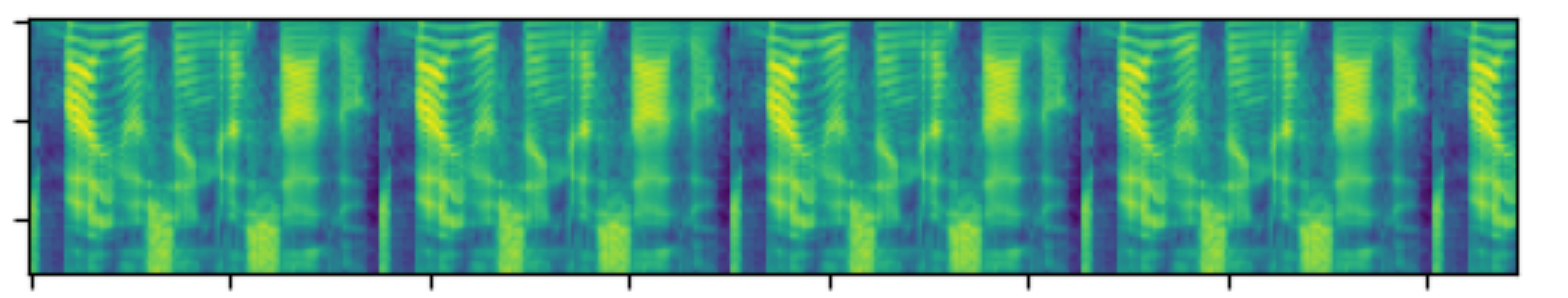
\includegraphics[width=0.9\linewidth]{figures_ning/mel-1}
	\caption[log-Mel spectrogram]{log-Mel spectrogram}
	\label{fig:mel-1}
\end{figure}

For parameter optimization during our experiments, we train the defense model on the training set and test it on the development set; the defense model used to validate the test set is trained from the combined training and development sets.Herein, three CNN architectures are employed due to CNN models' strong capability to extract high-level features from log-Mel spectrogram images~\cite{zhao2018data}. The implemented CNN models contain a conventional CNN model with four convolutional layers (named as CNN-4), a ResNet model, and a VGG model.
The CNN-4 model contains, four convolutional layers $[64,128,256,512]$, a global max pooling layer, a fully connected layer, and a softmax layer for the final classification. The four convulutional layers have a kernel with a size of $(5, 5)$, and each convulutional layer is followed by a local max pooling layer with a kernel size of $(2, 2)$. The global max pooling has shown better performance than flattening in our previous study~\cite{ren2018attention}, as it can extract smaller feature vectors from feature maps for classification.
Besides the CNN-4 model, another two state-of-the-art CNN models, ResNet and VGG, are employed for a comparison. ResNet~\cite{szegedy2017inception} contains the Inception architecture which requires relatively low computational cost. ResNet has shown promise in the tasks of image processing~\cite{szegedy2017inception}. ResNet has a series of structures with different numbers of layers. One of them, ResNet-50 ~\cite{he2016deep}, is utilised, since our work is focusing on adversarial attacks and training. Moreover, VGG has shown good performance on processing spectrogram images for audio classification tasks due to its deep architecture~\cite{simonyan2015very,ren2018learning}. Hence, we also train a VGG-16 model for this speech-based emotion recognition task.

\begin{table}[]
	\centering
	\begin{tabular}{c|c}
		\hline
		\#        & Probability    \\ \hline
		CNN-4     & surprise:0.995 \\ \hline
		VGG-16    & surprise:0.988 \\
		ResNet-50 & surprise:0.997
	\end{tabular}
	\caption[label of log-Mel spectrogram]{label of log-Mel spectrogram}
\end{table}

\section{Evaluation Metrics}
When training the black-box attack model in this study, the attacker does not know the parameters of the target model. The input data is first fed to the attack model to generate fake data, similar to the original input data (Figure 1(a)). The target model (i.e., the defense) is then unable to generate correct predictions for the generated data.
Regarding the inputs, log-Mel spectrograms are used due to their powerful performance in \textbf{SER}~\cite{ren2020generating,zhang2017speech} tasks. The real log-Mel spectrogram and labels are represented as $(x, y)$ and the generated adversarial data is$x^{\prime}$. The CNN model can then be trained to output a two-dimensional adversarial perturbation η. Finally, the adversarial data is obtained by $x^{\prime}=x+\eta$. Due to the ability to output features, an atrous CNN model is proposed to generate mappings with adversarial perturbations of the same size as the input~\cite{ren2019attention}. Efficient training of aerobic
CNN attack model, the loss function has two objectives: one is to deceive the defense $f$, and the other is to minimize the difference between fake and real data. Thus, the loss function is a weighted sum of the loss functions of the two objectives:
$$
\begin{gathered}
	\operatorname{loss}=\operatorname{\alpha oss}_{\text {cla }}\left(f\left(\boldsymbol{x}^{\prime}\right)\right)+(1-\alpha) \operatorname{loss}_{M S E}\left(\boldsymbol{x}^{\prime}, \boldsymbol{x}\right) \\
	\operatorname{loss}_{c l a}\left(f\left(x^{\prime}\right)\right)=\max \left(f\left(x^{\prime}\right)_{l}-\max \left(f\left(x^{\prime}\right)_{\text {other }}\right), 0\right)
\end{gathered}
$$

where $\alpha$ is the hyperparameter that balances the two loss functions $\operatorname{loss}_{c l a}$ and $\operatorname{loss}_{M S E}$. The loss function $\operatorname{loss}_{c l a}$ aims to reduce the defensive classification performance on false data, and $\operatorname{loss}_{M S E}$ aims to improve the similarity between false and true data using mean square error (MSE). The function losscla is defined by the difference between the probability of the correct label l and the maximum probability of the other classes. The calculation of losscla is known as the Carlini-Wagner $(\mathrm{C} \& \mathrm{~W})$ loss function~\cite{bose2018adversarial}. This approach has been used to generate adversarial attacks in image processing tasks~\cite{akhtar2018threat,bose2018adversarial}.
The log-Mel spectrogram after the attack model is as follows:
\begin{figure}[!hbtp]
	\centering
	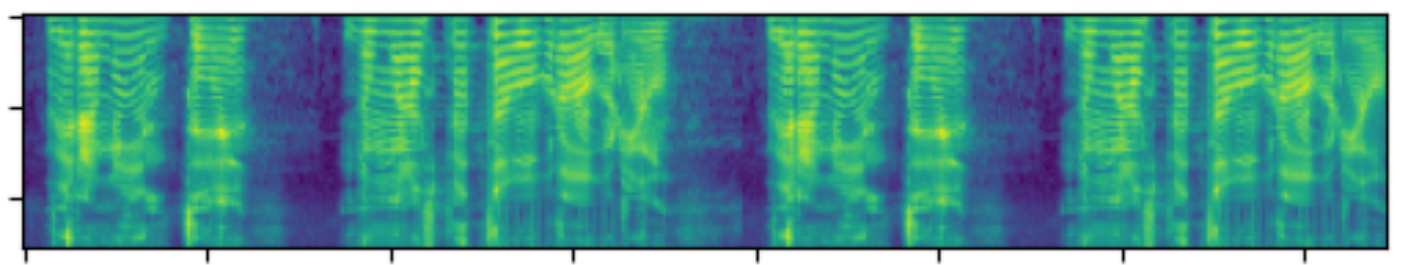
\includegraphics[width=0.9\linewidth]{figures_ning/mel-2}
	\caption[Fake log-Mel spectrogram]{Fake log-Mel spectrogram}
	\label{fig:mel-2}
\end{figure}

\begin{figure}[!hbtp]
	\centering
	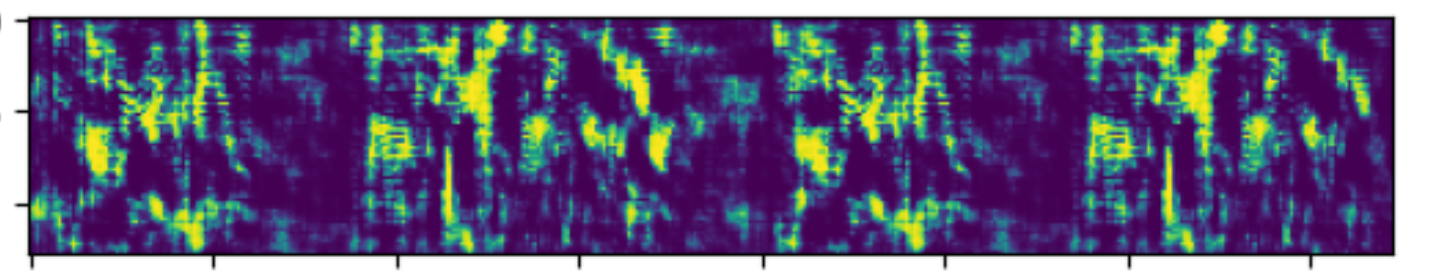
\includegraphics[width=0.9\linewidth]{figures_ning/mel-3}
	\caption[Adversarial perturbation]{Adversarial perturbation}
	\label{fig:mel-3}
\end{figure}

\begin{figure}[!hbtp]
	\centering
	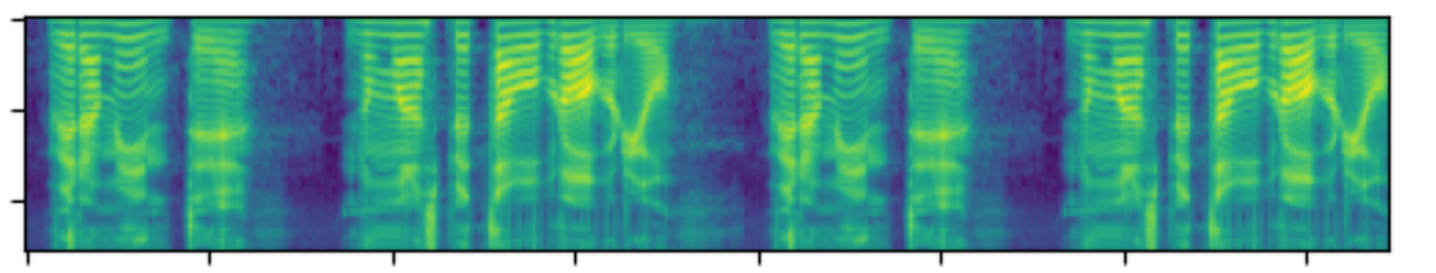
\includegraphics[width=0.9\linewidth]{figures_ning/mel-4}
	\caption[Real log-Mel spectrogram]{Real log-Mel spectrogram}
	\label{fig:mel-4}
\end{figure}

After that we use the changed spectrogram as input and re-judged by the three defense models to obtain the following results:
\begin{table}[!h]
	\centering
	\begin{tabular}{c|c|c}
		\#        & Probability of Real log-Mel spectrogram & Probability of Fake log-Mel spectrogram \\ \hline
		CNN-4     & Surprise:0.995                          & Guilt:0.586                             \\
		VGG-16    & Surprise:0.988                          & Anger:0.878                             \\
		ResNet-50 & Surprise:0.997                          & Anger:0.788                            
	\end{tabular}
	\caption[Classification of log Mel spectrogram]{Classification of log Mel spectrogram}
	\label{tab:log-2}
\end{table}

This proves the success of the attack. The original audio message(log-Mel spectrogram) was classified as Surprise, and after the attack model we designed, it became Guilt or Anger. we don't care about the specific category of the final classification, as long as it doesn't match the original label, it shows the success of our black box attack.

For the presentation of the final experimental results, the Unweighted Average Recall (UAR), which is an unweighted average result, is used as an evaluation metric considering the category imbalance. This is because the classifier of the defense model has seven labels, but each label corresponds to a different number of audio files. Our purpose is to judge the accuracy of each emotion, and if we directly use all the number of labels to judge the accuracy, it will produce a large error. For example, if the data is divided unevenly, there are 3847 messages in the training set, among which there are 2000 Angry labels, so that the proportion of Angry labels is much higher than 1/7. If our attack model has good aggressiveness for angry audio messages, if the final accuracy obtained by the defense model is only 0.100, but the aggressiveness for other audio messages is poorer If we use the average accuracy directly, the result is 0.302, as in Table~\ref{tab:dir}; however, if we use UAR calculation, as in Table 2, the result is 0.461~\ref{tab:uar}. 
\begin{table}[!hbtp]
	\centering
	\subtable[Directly Average Accuracy]{
		\begin{tabular}{l|ll}
			\centering
			Scene Label   & Number & Accuracy \\ \hline
			Anger         & 2000   & 0.100    \\
			Other Emotion & 1847   & 0.521    \\
			Sum           & 3847   & 0.302   
			\label{tab:dir}
	\end{tabular}}
	\subtable[Unweighted Average Recall]{
		\begin{tabular}{l|ll}
			Scene Label   & Number & Accuracy \\ \hline
			Anger         & 2000   & 0.100    \\
			Other Emotion & 1847   & 0.521    \\
			Sum           & 3847   & 0.461   
			\label{tab:uar}
	\end{tabular}}
	\caption{Different Result}
	\label{tab:diff}
\end{table}

The difference between the two is very large. Such a result can only show that the attack model has obvious effect on specific audio files, but we are judging seven kinds of tags, and obviously UAR is suitable as a judgment criterion.
The following table is an example of UAR as a judgment criterion, first finding the accuracy rate of each tag, and then finding the average of the seven labels:
\begin{table}[!hbtp]
	\centering
	\begin{tabular}{l|ll}
		Scene Label & Number & Accuracy \\ \hline
		Anger       & 431    & 0.752    \\
		Disgust     & 487    & 0.827    \\
		Fear        & 643    & 0.766    \\
		Guilt       & 721    & 0.737    \\
		Happiness   & 274    & 0.817    \\
		Sadness     & 523    & 0.705    \\
		Surprise    & 768    & 0.847    \\ \hline
		Average     & 3847   & 0.779   
	\end{tabular}
	\caption{Unweighted Average Recall Of CNN-4}
	\label{tab:UAR}
\end{table}


\label{sec:experimentpixel}
\section{Experiments on Dynamic Neural Networks}
In Section~\ref{sec:pixel_base}, we put forward related ideas, through the attention map in Fig.~\ref{fig:method1baseline} to find possible relationships in the detected pictures. We hope that the most relevant area can be directly reflected in the attention map, so we designed an attention loss function(see Eq.~\ref{pixel_attention_loss}) so that the attention weights of the relevant area are higher than the non-relevant area.

We tried to add a multi-head self-attention module after obtaining the image feature in VGG16 based on the code of RelDN~\cite{zhang2019graphical},  so that we obtained a new image feature with a size of $ [bs, 512, 50, 66]  $and an  attention map with a size of $ [bs, 3300, 3300] $, where bs is batch size=2. We build the baseline as the Fig.~\ref{fig:method1baseline} shown.

\subsubsection{Result of the Pixel Attention Loss  Function}
Figure~\ref{fig:singlepixelmap} shows the attention map of a single pixel after loss function processing. The attention weights between each pixels of subject and the entire image is computed, which can be expressed as $ \forall Attention_{p^k_{sbj} \to p^i_{img}} , p^i_{img} \in \mathbb{P}_{img} $, where k is the $ k^{th} $ pixel of the subject.

\begin{figure}[h!]
	\centering
	\subfigure[$ <arm, on, man> $]{
		\begin{minipage}[t]{3.5cm}
			\centering
			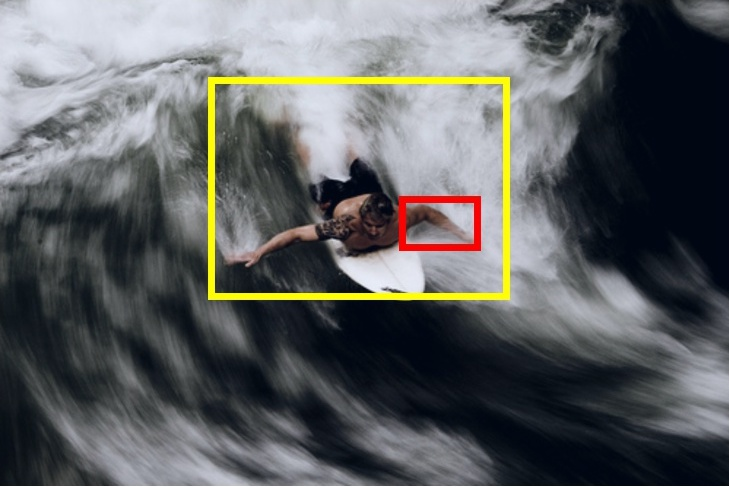
\includegraphics[width=0.9\linewidth]{figures/pixel/img2}
		\end{minipage}
		\begin{minipage}[t]{3.5cm}
			\centering
			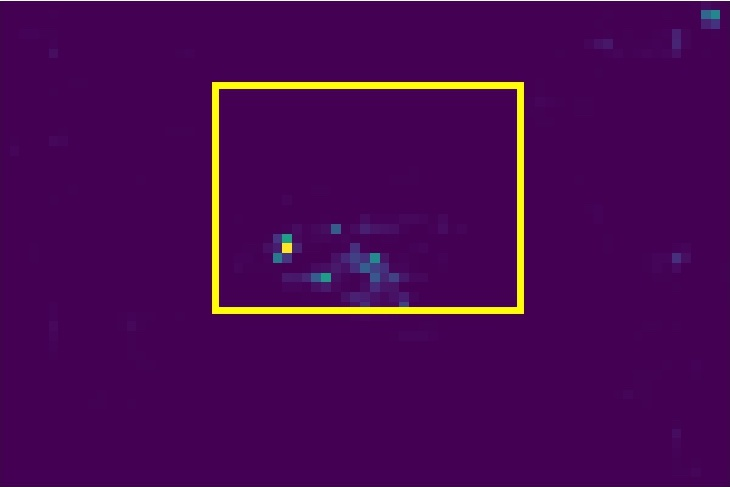
\includegraphics[width=0.9\linewidth]{figures/pixel/map2_1}
		\end{minipage}
		\begin{minipage}[t]{3.5cm}
			\centering
			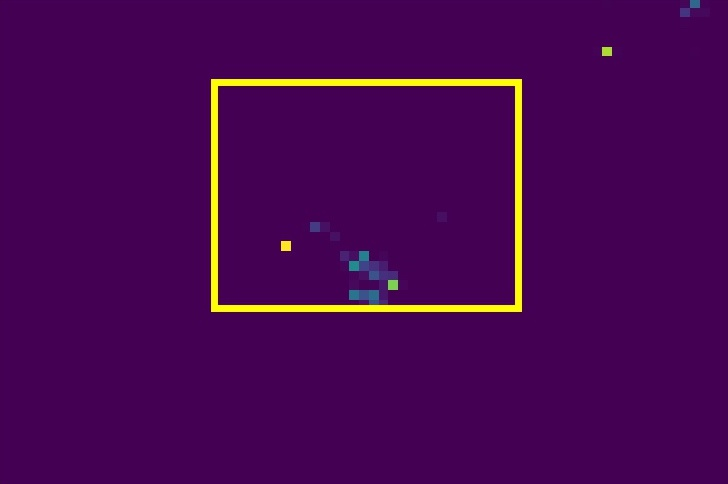
\includegraphics[width=0.9\linewidth]{figures/pixel/map2_2}
		\end{minipage}
		\begin{minipage}[t]{3.5cm}
			\centering
			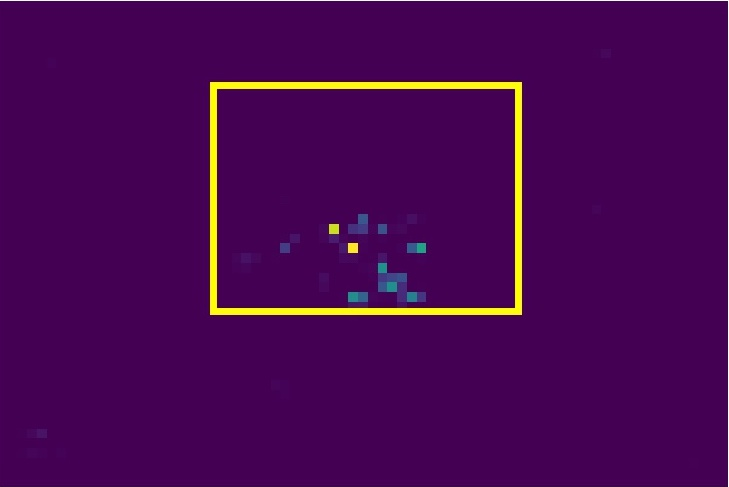
\includegraphics[width=0.9\linewidth]{figures/pixel/map2_3}
		\end{minipage}
		\label{fig:singlepixelmap_a}}
	
	\subfigure[$ <bike, has, wheel> $]{
		\begin{minipage}[t]{3.5cm}
			\centering
			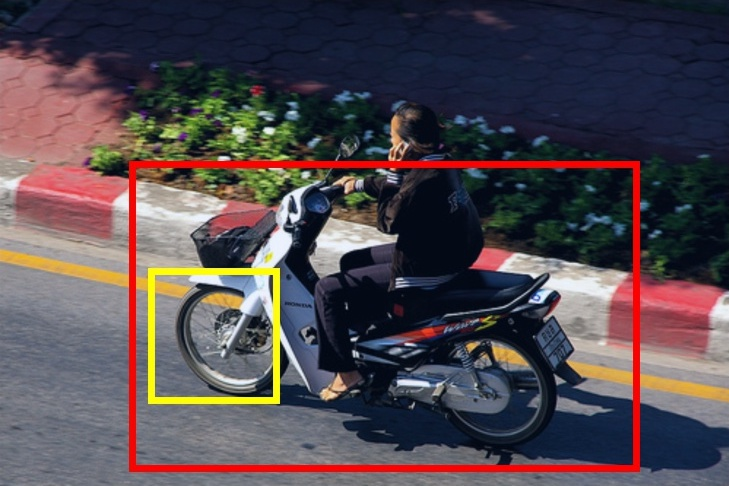
\includegraphics[width=0.9\linewidth]{figures/pixel/img3}
		\end{minipage}
		\begin{minipage}[t]{3.5cm}
			\centering
			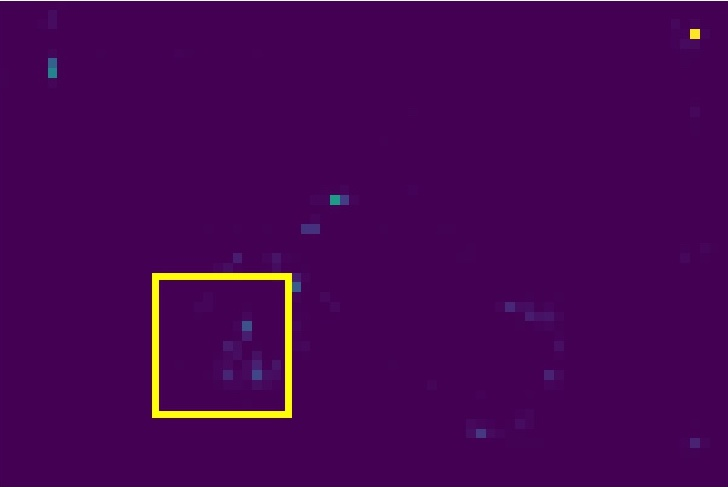
\includegraphics[width=0.9\linewidth]{figures/pixel/map3_1}
		\end{minipage}
		\begin{minipage}[t]{3.5cm}
			\centering
			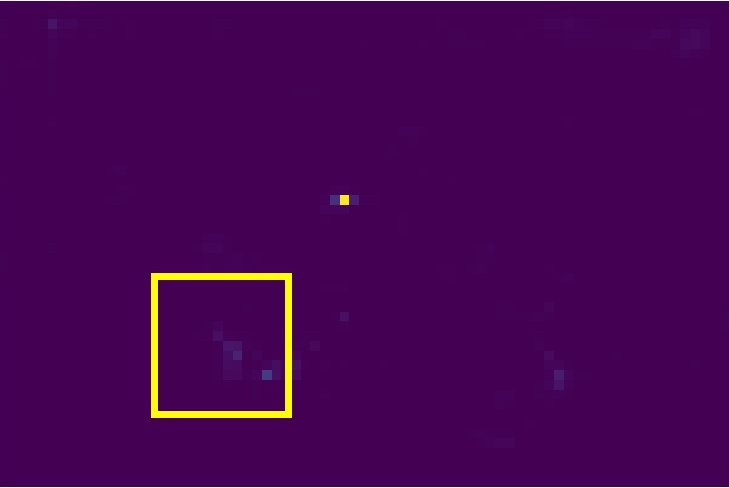
\includegraphics[width=0.9\linewidth]{figures/pixel/map3_2}
		\end{minipage}
		\begin{minipage}[t]{3.5cm}
			\centering
			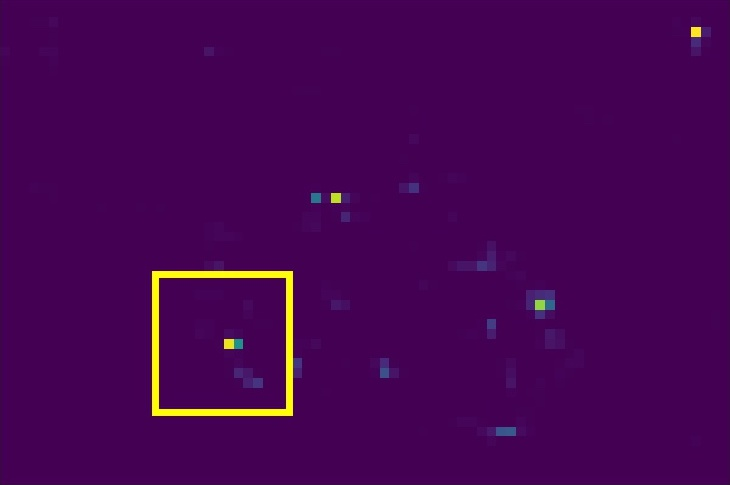
\includegraphics[width=0.9\linewidth]{figures/pixel/map3_3}
		\end{minipage}
		\label{fig:singlepixelmap_b}}
	
	
	\subfigure[$<window, on, door>$]{
		\begin{minipage}[t]{3.5cm}
			\centering
			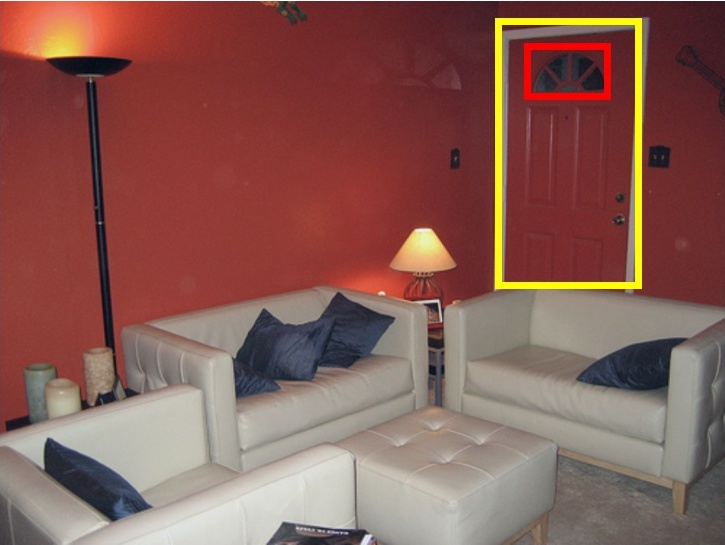
\includegraphics[width=0.9\linewidth]{figures/pixel/img4}
		\end{minipage}
		\begin{minipage}[t]{3.5cm}
			\centering
			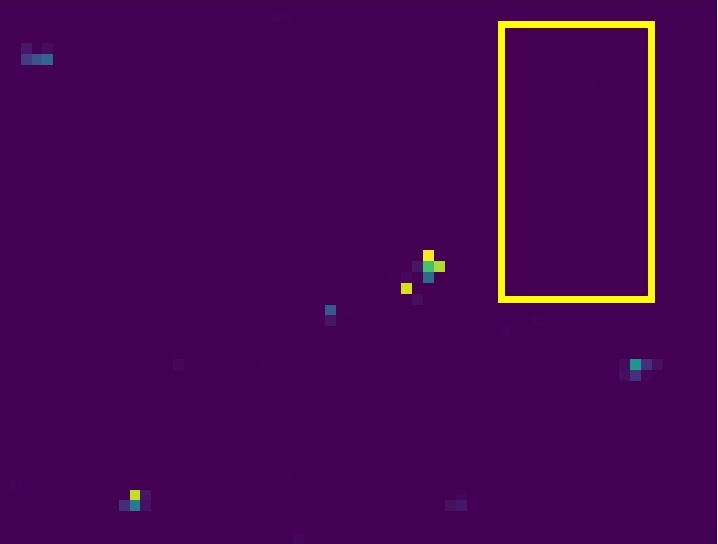
\includegraphics[width=0.9\linewidth]{figures/pixel/map4_1}
		\end{minipage}
		\begin{minipage}[t]{3.5cm}
			\centering
			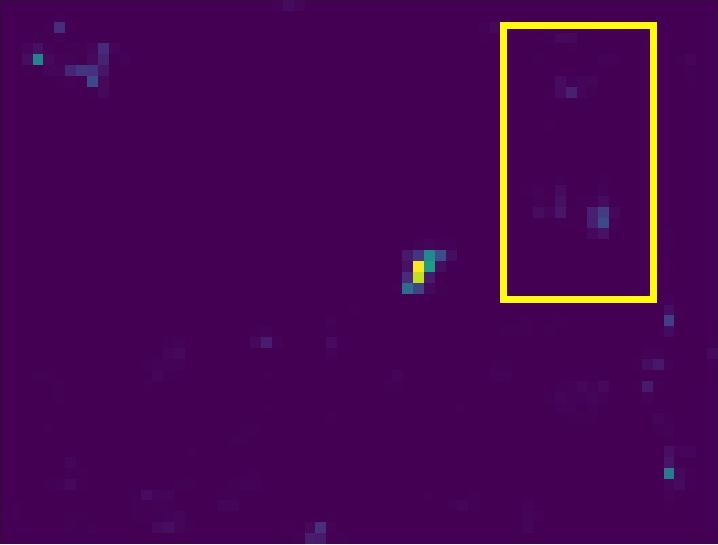
\includegraphics[width=0.9\linewidth]{figures/pixel/map4_2}
		\end{minipage}
		\begin{minipage}[t]{3.5cm}
			\centering
			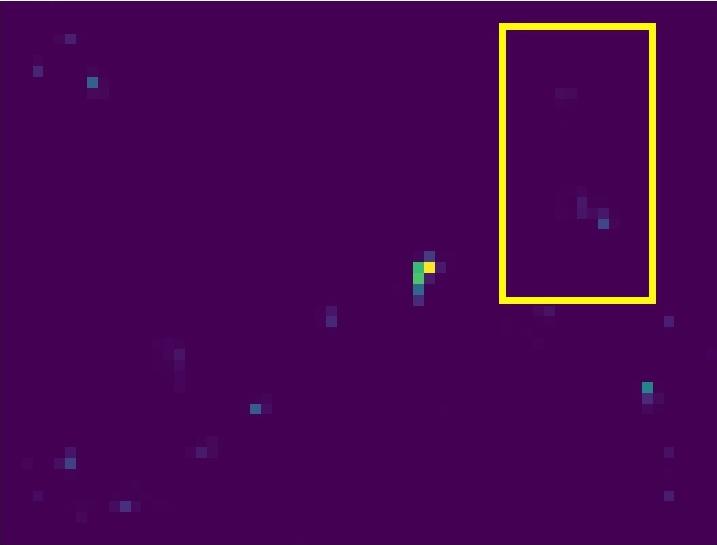
\includegraphics[width=0.9\linewidth]{figures/pixel/map4_3}
		\end{minipage}
		\label{fig:singlepixelmap_c}}
	
	\subfigure[ $<zebra, has, leg>$]{
		\begin{minipage}[t]{3.5cm}
			\centering
			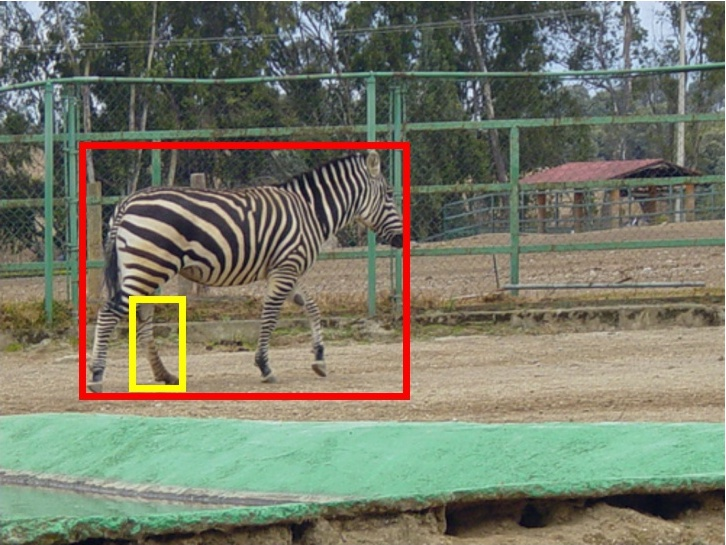
\includegraphics[width=0.9\linewidth]{figures/pixel/img5}
		\end{minipage}
		\begin{minipage}[t]{3.5cm}
			\centering
			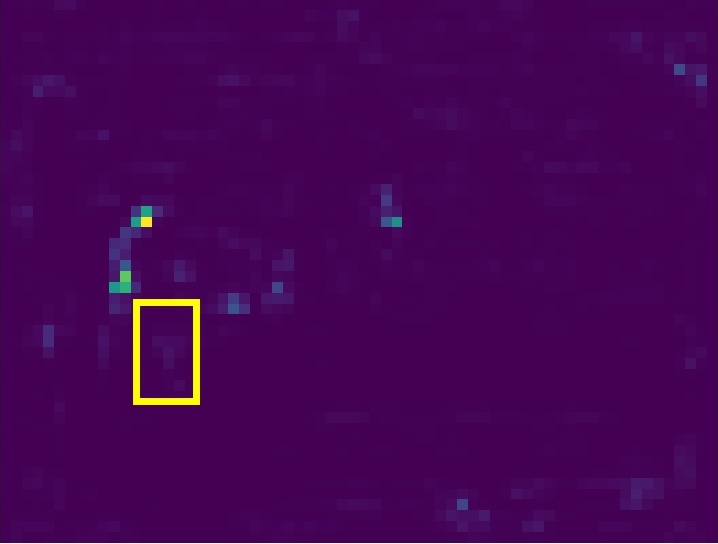
\includegraphics[width=0.9\linewidth]{figures/pixel/map5_1}
		\end{minipage}
		\begin{minipage}[t]{3.5cm}
			\centering
			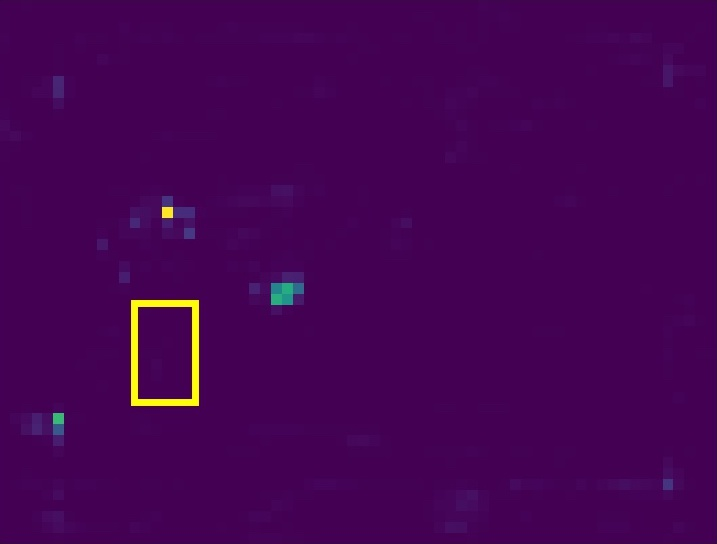
\includegraphics[width=0.9\linewidth]{figures/pixel/map5_2}
		\end{minipage}
		\begin{minipage}[t]{3.5cm}
			\centering
			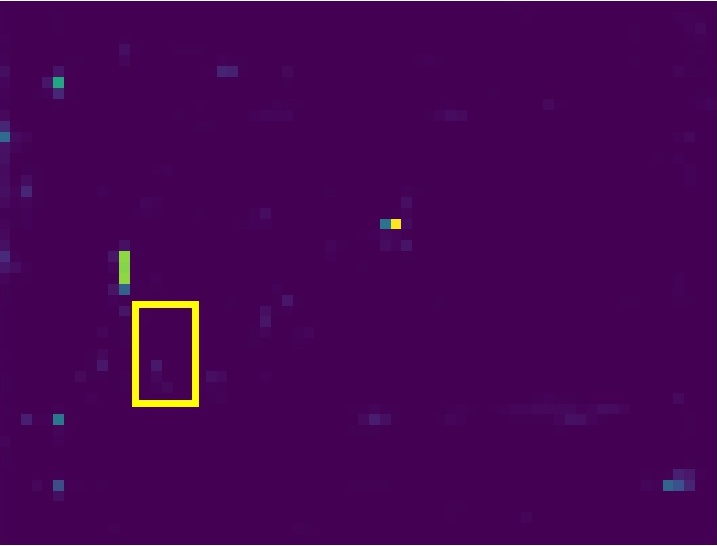
\includegraphics[width=0.9\linewidth]{figures/pixel/map5_3}
		\end{minipage}
		\label{fig:singlepixelmap_d}}
	
	\caption[Visualized results of the attention map of a single pixel ]{Visualized results of the attention map of a single pixel. The red box in the figure is subject, and the yellow box is object. We randomly select a few pixels from the subject, then draw the attention map of these pixels to the entire picture. }
	\label{fig:singlepixelmap}
\end{figure}

As shown in Figure~\ref{fig:singlepixelmap_a}, we randomly select three pixels from subject \textit{arm} and drew their attention weights map for the entire image, the red box is the subject \textit{arm} and the yellow box is the object\textit{ man}, and the ground truth relation is \textit{arm on man}. In the picture, the most highlights are in the yellow box, which means that these pixels of the subject focus more on the object \textit{man}. Although the loss function performs well in Figure (a), it works not well with the other picture, such as the Figure (b), (c), (d).

In Figure~\ref{fig:singlepixelmap_b}, the subject is \textit{bike}, and the object is \textit{wheel}. We also select three pixels from the subject and draw their attention maps. In the three attention maps, most of the highlights are out of the yellow box, which means that the pixels of subject \textit{bike} pays little attention the object \textit{wheel}, and from the distribution of the highlights it can be find that the pixels pay more attention to the rest part of the subject \textit{bike}.

In Figure~\ref{fig:singlepixelmap_c}, the subject is \textit{window}, and the object is \textit{door}. In the attention maps, the pixels of  \textit{window} pay nor attention to the subject or the object. They focus on the lamps, which has no relation with the subject \textit{window}.

The attention maps of Figure~\ref{fig:singlepixelmap_d} shows that some pixels of subject \textit{zebra} focus on the subject and some of them focus on the parts of the image except the subject and object.

After analyzing the result of the experiments, it comes to a conclusion that this loss function performs not well. With this loss function, most $ \forall Att_i^{rel} $ are not able to reflect the relation between subjects and objects. The results show that most of subjects can not pay attention to the right objects, they focus more on themselves or the parts that has no relation to them.



\begin{figure}[!h]
	\centering
	\subfigure[Image input.]{
		\begin{minipage}[t]{7.5cm}
			\centering
			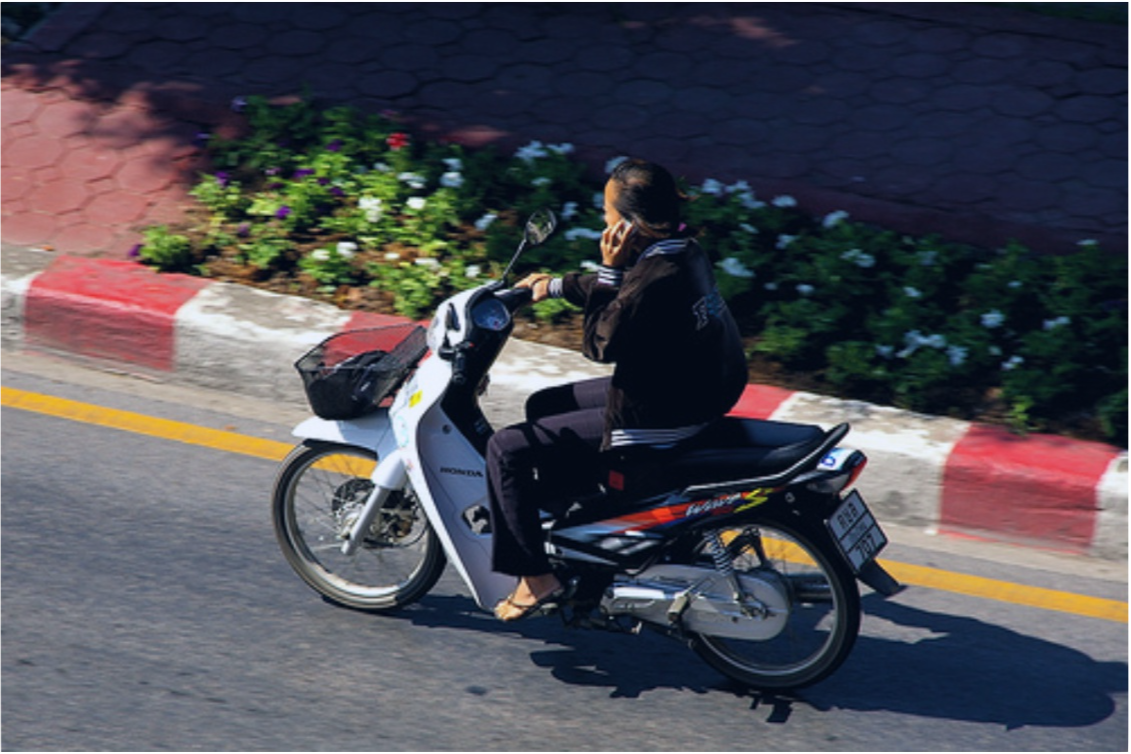
\includegraphics[width=0.95\linewidth]{figures/motor/img}
			\label{fig:motor_img}
	\end{minipage}}
	\subfigure[The result of a normalized attention map.]{
		\begin{minipage}[t]{7.5cm}
			\centering
			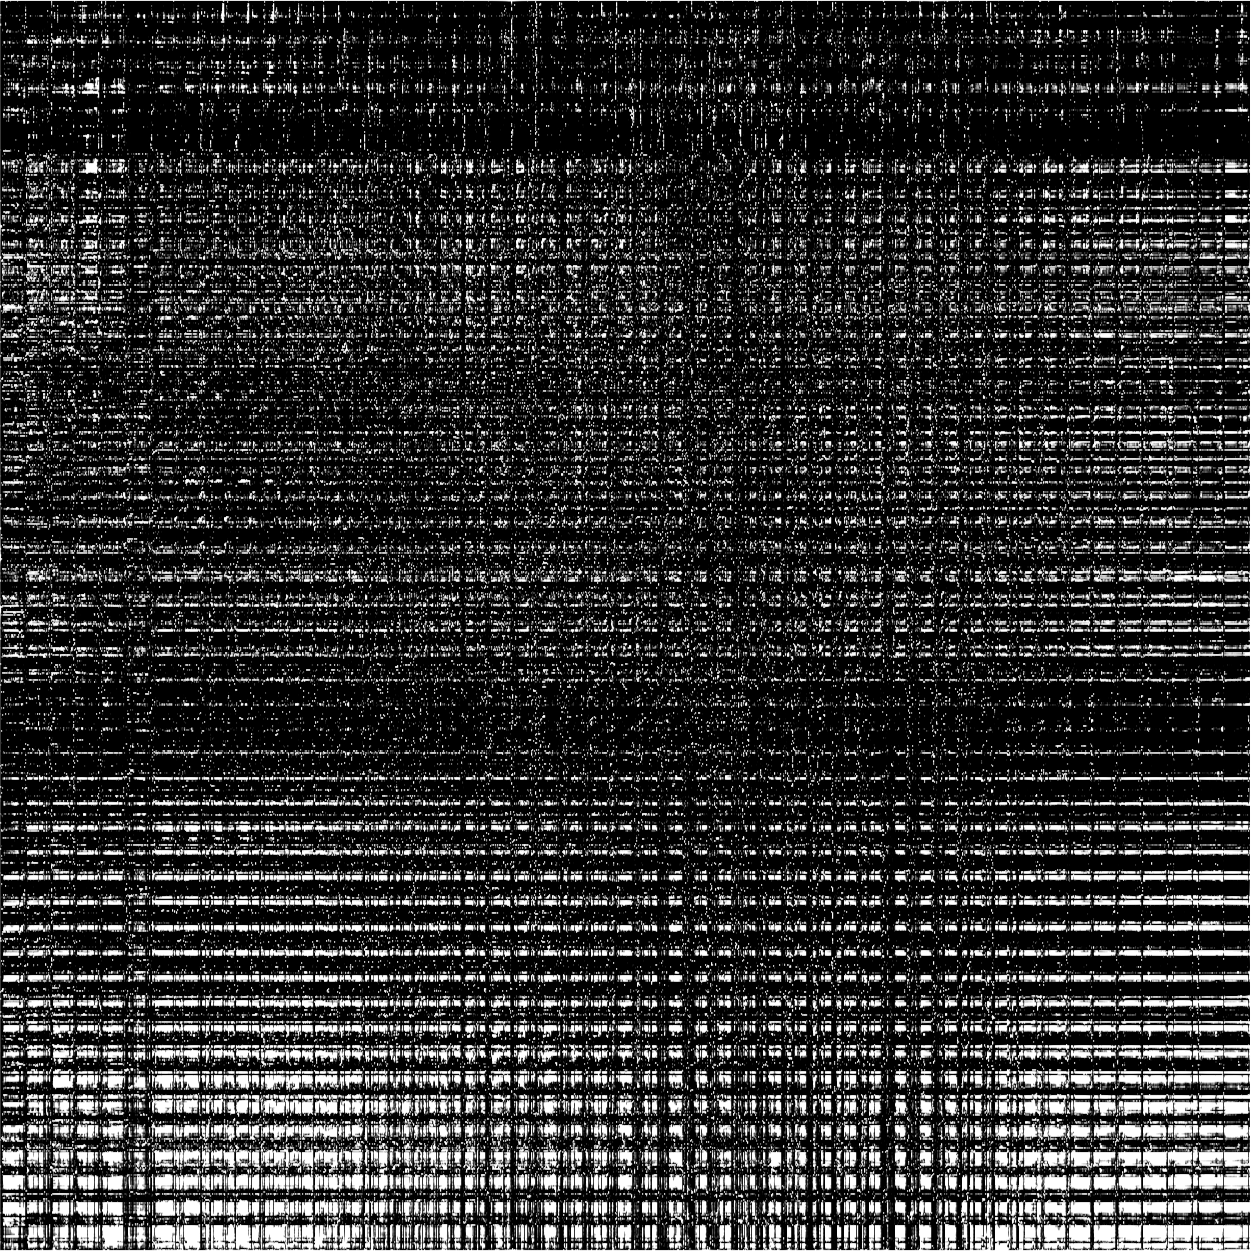
\includegraphics[width=0.8\linewidth]{figures/motor/attention}
			\label{fig:motor_attention_map}
	\end{minipage}}
	
	\caption[The result of a normalized attention map drawn by matlab]{The result of a normalized Attention Map drawn by matlab.}
	\label{fig:motor_attention}
\end{figure}

\subsubsection{Result analysis}

In order to find the cause of the above problem, the complete attention map of the Fig.~\ref{fig:motor_img} is drawn in Figure~\ref{fig:motor_attention_map}. It can be seen from the figure that the overall distribution of $ \forall Attention_{p^i_{img} \to p^j_{img}} , p^i_{img},p^j_{img} \in \mathbb{P}_{img} $ is still relatively uniform, and it is not intuitive to distinguish which objects have a relationship. It can only indicate that the loss function has changed the attention map, but this change has no benefits to the relationship detection.

Then Figure~\ref{fig:motor_pair}  shows the position about the attention weights set for each relation pair. Figure(d) shows the position of $ \forall Attention_{p^i_{man} \to p^j_{bike}} $ ,  $ \forall Attention_{p^i_{man} \to p^j_{bike}} \in \forall Att_{rel} $ in the attention map. Because the whole bike is the ground truth object, the loss function should increase its attention weights. While the white areas in Figure(e) and Figure (f) belong to $ \forall Att_{no\_rel} $, which means that the man and wheels have no intersection in this scene, the loss function should lower its attention weights.

 In Figure~\ref{fig:motor_pair}(a)(b)(c), the subject is \textit{man} and the objects are \textit{bike}, \textit{$ wheel_1 $}, \textit{$ wheel_2 $}, \textit{$ wheel_1 $} and \textit{$ wheel_2 $} belong to \textit{bike}, and there is overlap between bike and wheels. It causes that the sets of attention weights for these three relation pairs also have overlap, so this loss function cannot highlight the attention weights of $ \forall Attention_{p^i_{man} \to p^j_{bike}} $ while reducing the attention weights of  $ \forall Att_{no\_rel} $.

This overlap is so serious and in Figure~\ref{fig:overlap} there is an example analyze.The white area in Figure~\ref{fig:overlap}(a) is the position of set of all relation pairs$ Att_{rel} $  about the image in the attention map, and the white area in Figure~\ref{fig:overlap}(b)  are position of the set of all no relation pairs $ Att_{no\_rel} $.When we calculate the overlap between $Att_{rel} $ and  $Att_{no\_rel} $, we can find that the white area of Figure(b) is contained in the white area of Figure(a). It can be expressed as  $$ \forall Att^i_{rel} \cap  \forall Att^i_{no\_rel } = \forall Att^i_{rel}  $$ or $$ \forall Att^i_{rel}  \subseteq  \forall Att^i_{no\_rel }$$.

This  overlap is not a special case, almost all pictures have this problem, so the pixel attention loss becomes meaningless. It cannot make the attention weights of the overlapping areas higher or lower so the idea of pixel-based attention can not go further, and it is not feasible to use the attention between pixels to obtain which relation pair is most likely to have a relationship.

%From the results, our attention loss has made certain modifications to the attention map. But in general, the values in the attention map are relatively average, and there is no strong distinguish ability. For instance, the ground truth pair $ <man, motorcycle>  $ shown in Fig.~\ref{fig:motor_man0}, its location of the corresponding area in attention map shown in Fig.~\ref{fig:motor_map0}. We can see the attention values in the area of the attention map(Fig.~\ref{fig:motor_attention_map}) is not higher than other areas, even be low.
%
%In general, we use our  average of attention weights  of each pair to replace the original pair score ($ score_{pair}=score_{subject }*score_{predicate}* score_{object} $) in the evaluation to sort relation pairs, and it does not improve the recall rate of the relation.
%
%Then we analyzed the results, and we drew the position of all $ Att_{rel} $s and all $ Att_{no\_rel} $s in the attention map of image~\ref{fig:motor_img} , see Fig.~\ref{fig:overlap} $ (a) $ and $ (b) $ in the figure. And the overlap between them is shown in Figure $ (c). $ We found that $ Att_{rel }$ and $ Att_{no\_rel} $ have a very serious overlap, and are basically the same as $ Att_{rel }$, that is,  $ Att_{no\_rel} $ contains $ Att_{rel }$. The purpose of our Attention Loss is to make $ Att_{rel }$ higher and $ Att_{no\_rel }$ lower. The existence of this overlap makes its purpose very contradictory. For example, the area in Figure~\ref{fig:motor_all0} belongs to $ Att_{rel }$ but it also belongs to $ Att_{no\_rel }$ in Figure~\ref{fig:motor_all1}. We cannot make it higher and lower. This overlap in the image is shown in Figure~\ref{fig:motor_pair}. For example, for the same subject $ man $, there are  pairs $<man,ride,motorcycle>$, $ <man, \varnothing, wheel_1> $  and  $ <man, \varnothing, wheel_2>  $, their objects have an overlap, and the bounding box  of $ motor $ obviously contains the bounding box of  $ wheel $.
%
%This overlap is not a special case. We found that almost all images have this situation, so the attention loss we designed is meaningless, and the idea of Piexl-based Attention also failed. We cannot use the attention between pixels to obtain which pair is most likely to have a relationship.

\begin{figure}[h!]
	\centering
	\subfigure[$<man,ride,bike>$]{
		\begin{minipage}[t]{5cm}
			\centering
			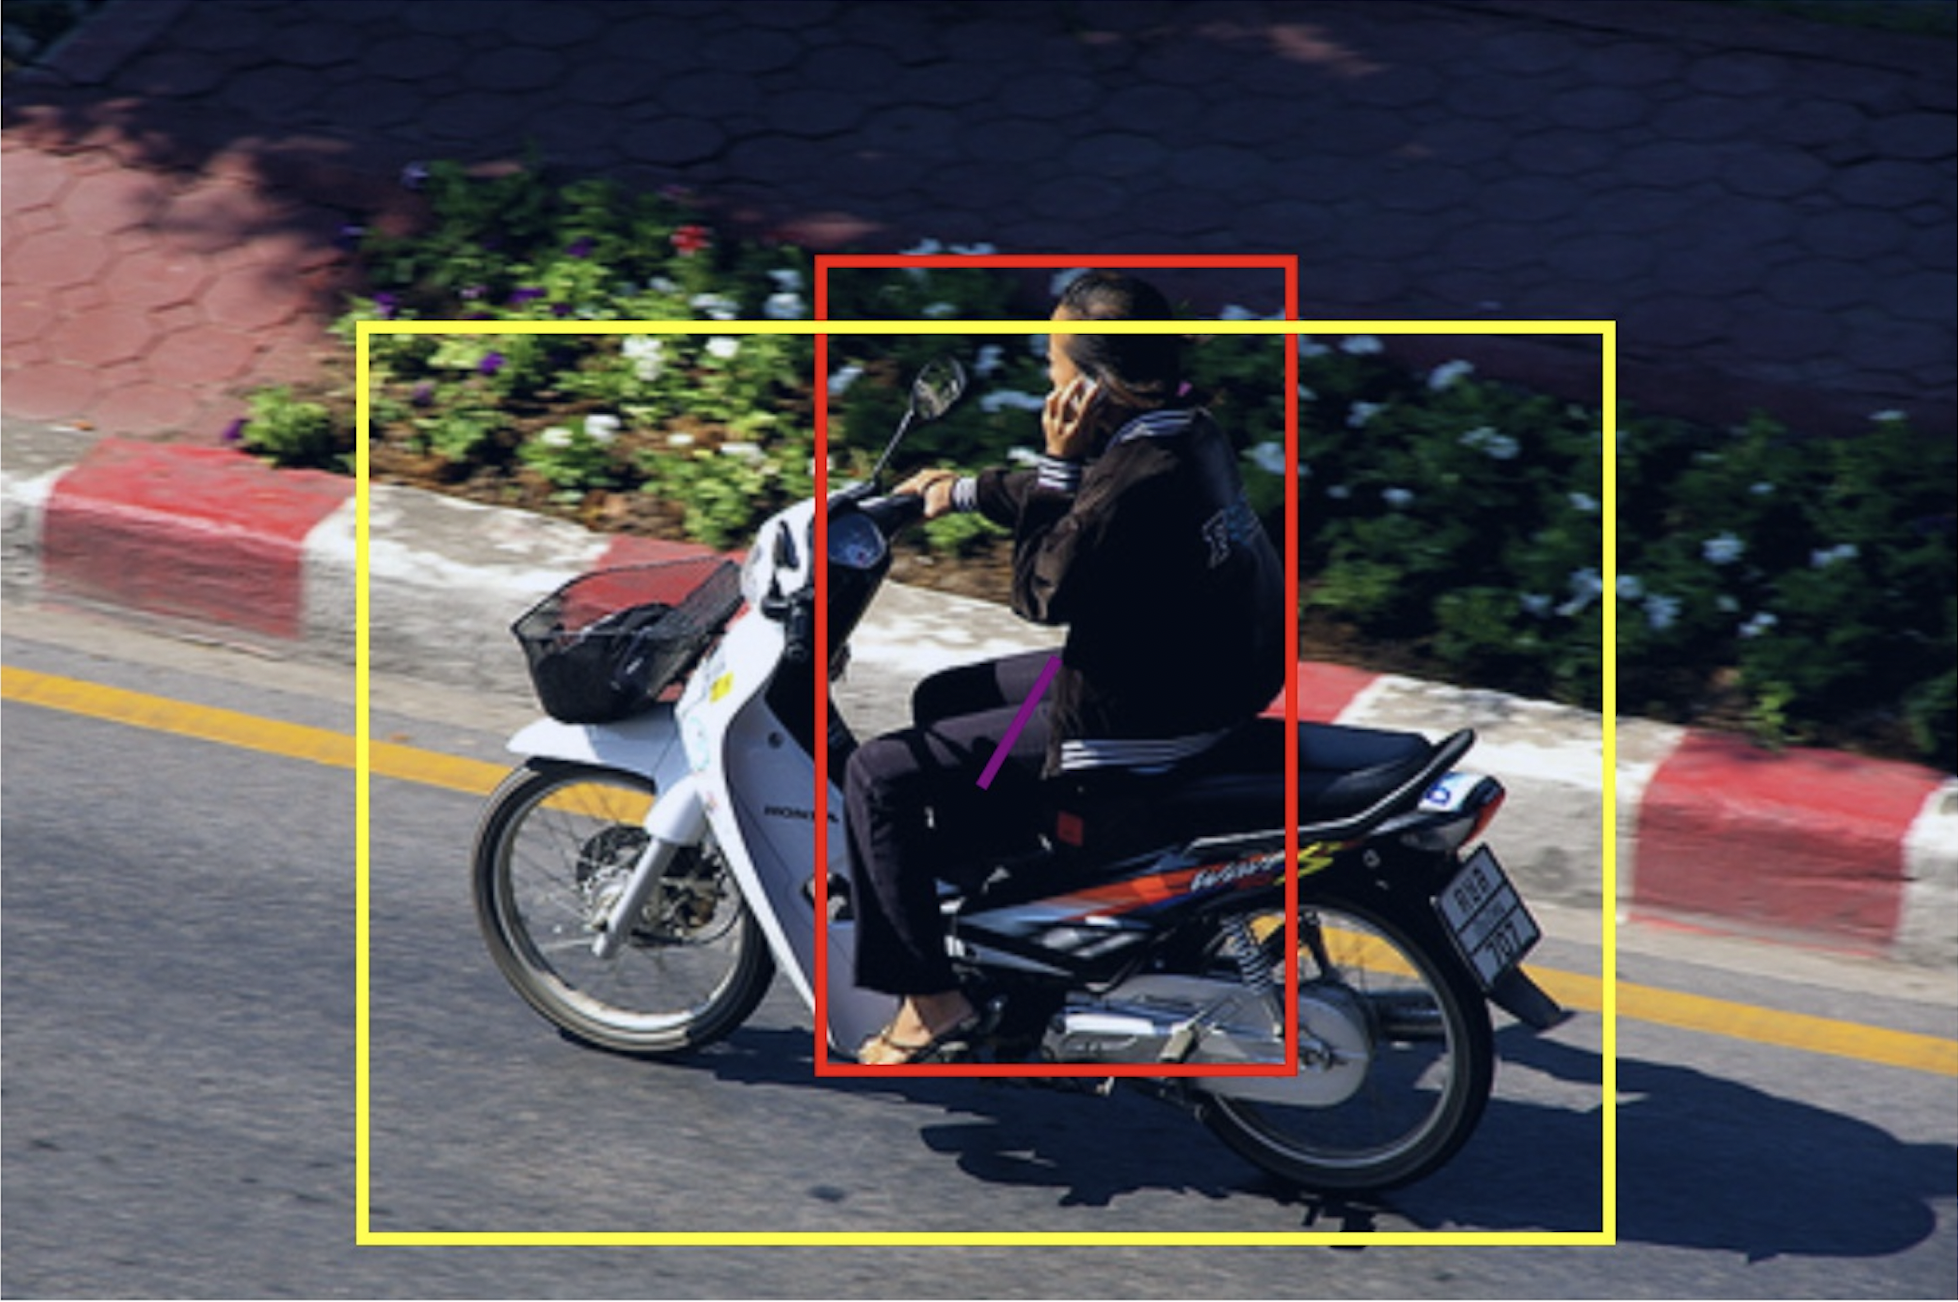
\includegraphics[width=0.9\linewidth]{figures/motor/man0}
			\label{fig:motor_man0}
	\end{minipage}}
	\subfigure[$ <man, \varnothing, wheel_1> $]{
		\begin{minipage}[t]{5cm}
			\centering
			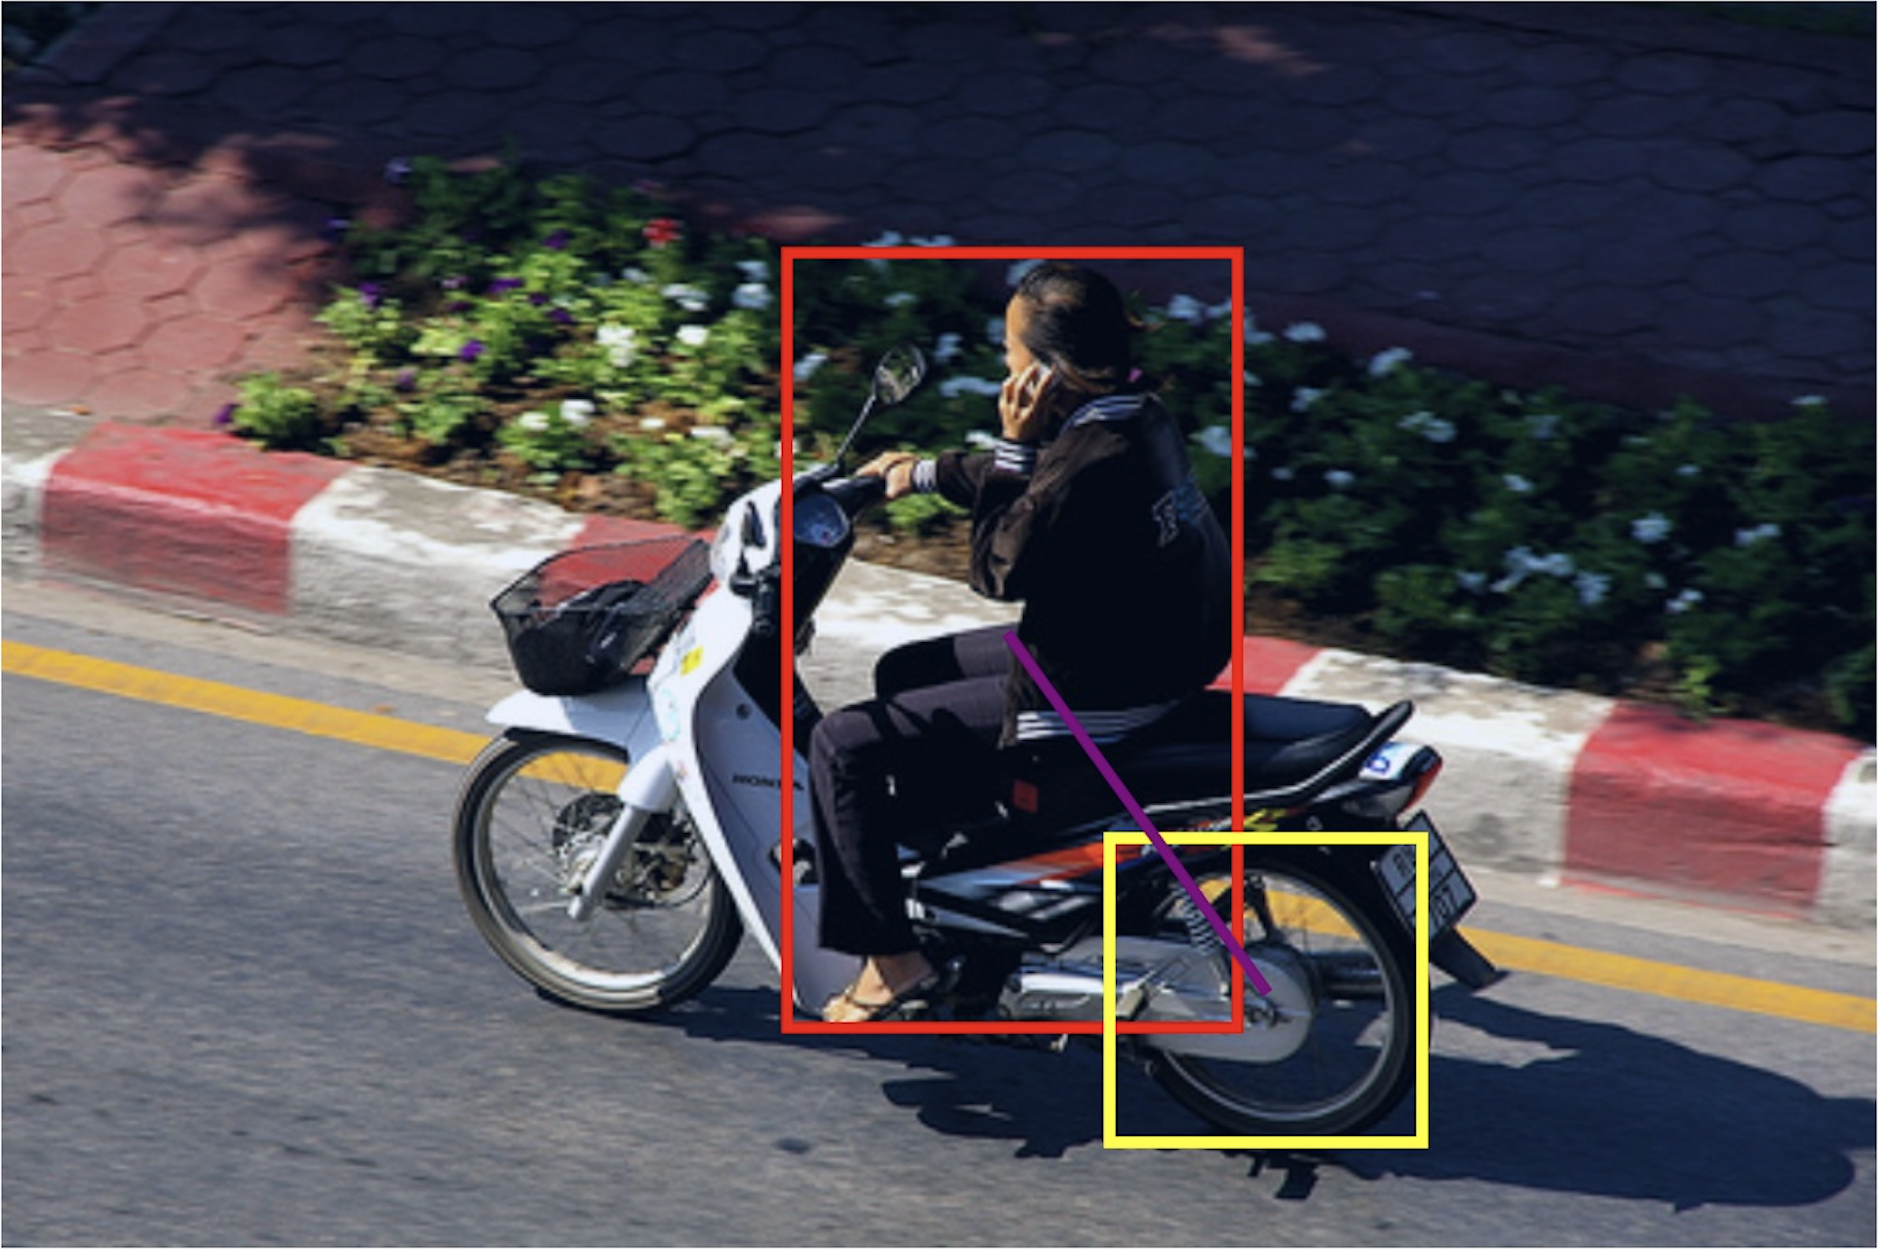
\includegraphics[width=0.9\linewidth]{figures/motor/man1}
			\label{fig:motor_man1}
	\end{minipage}}
	\subfigure[$ <man, \varnothing, wheel_2>  $]{
		\begin{minipage}[t]{5cm}
			\centering
			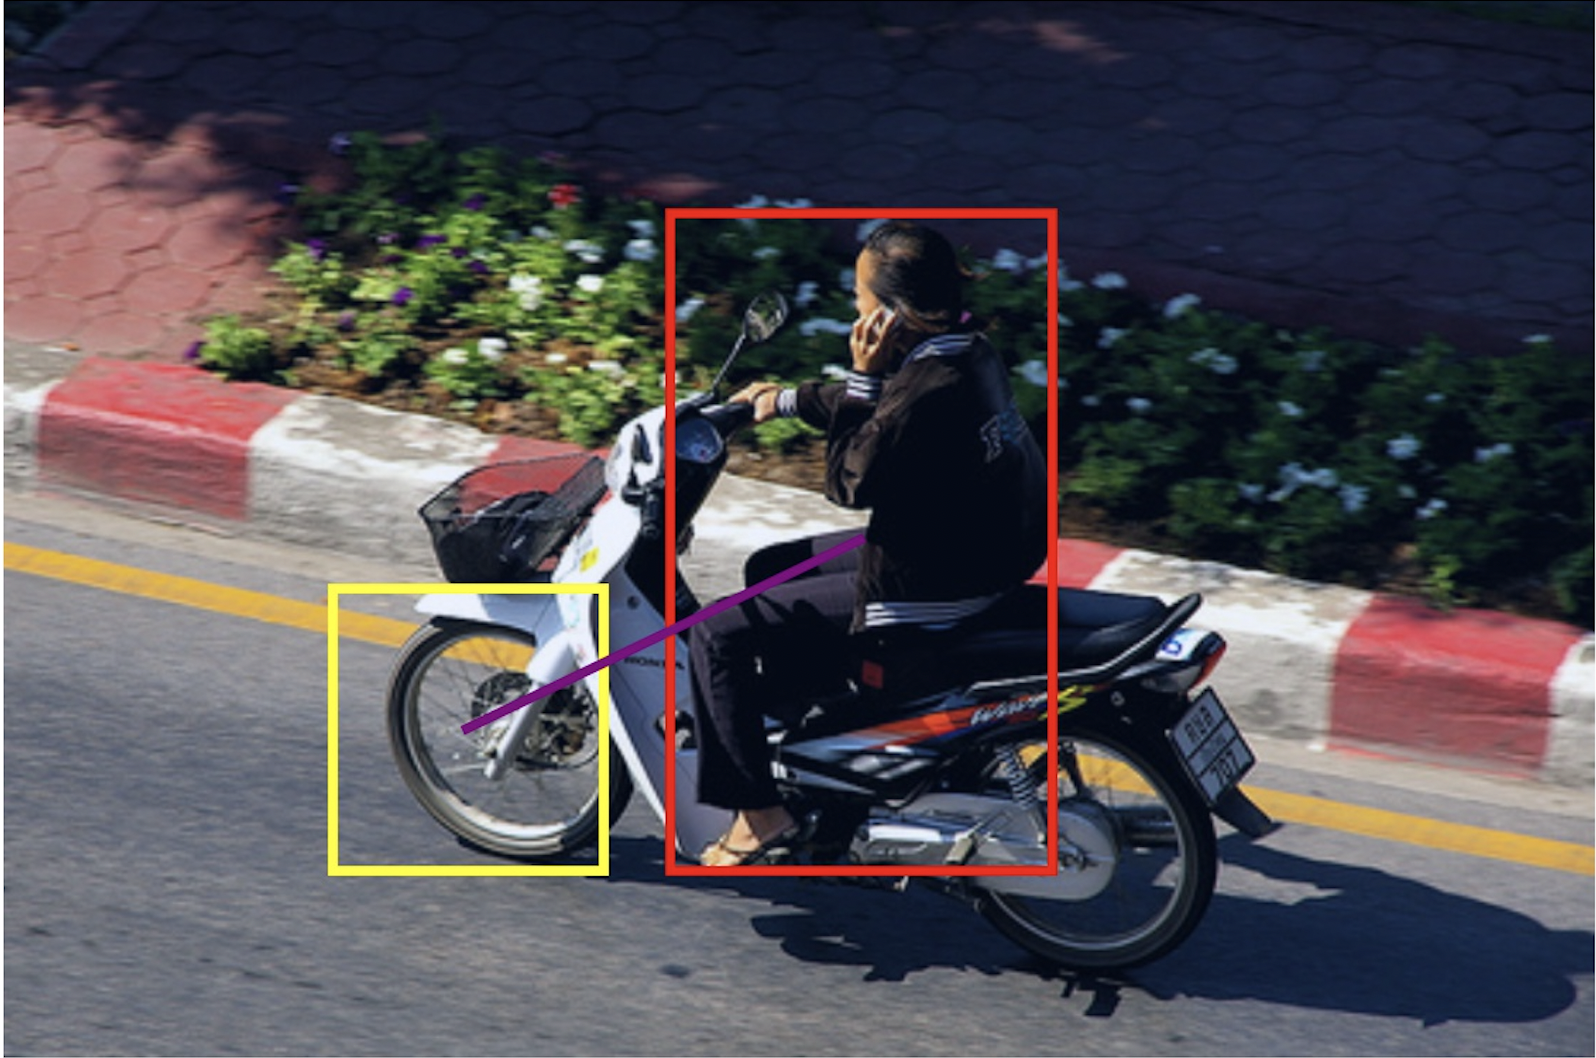
\includegraphics[width=0.9\linewidth]{figures/motor/man2}
			\label{fig:motor_man2}
	\end{minipage}}

	\subfigure[$\forall Attention_{p^i_{man} \to p^j_{bike}} $]{
		\begin{minipage}[t]{5cm}
			\centering
			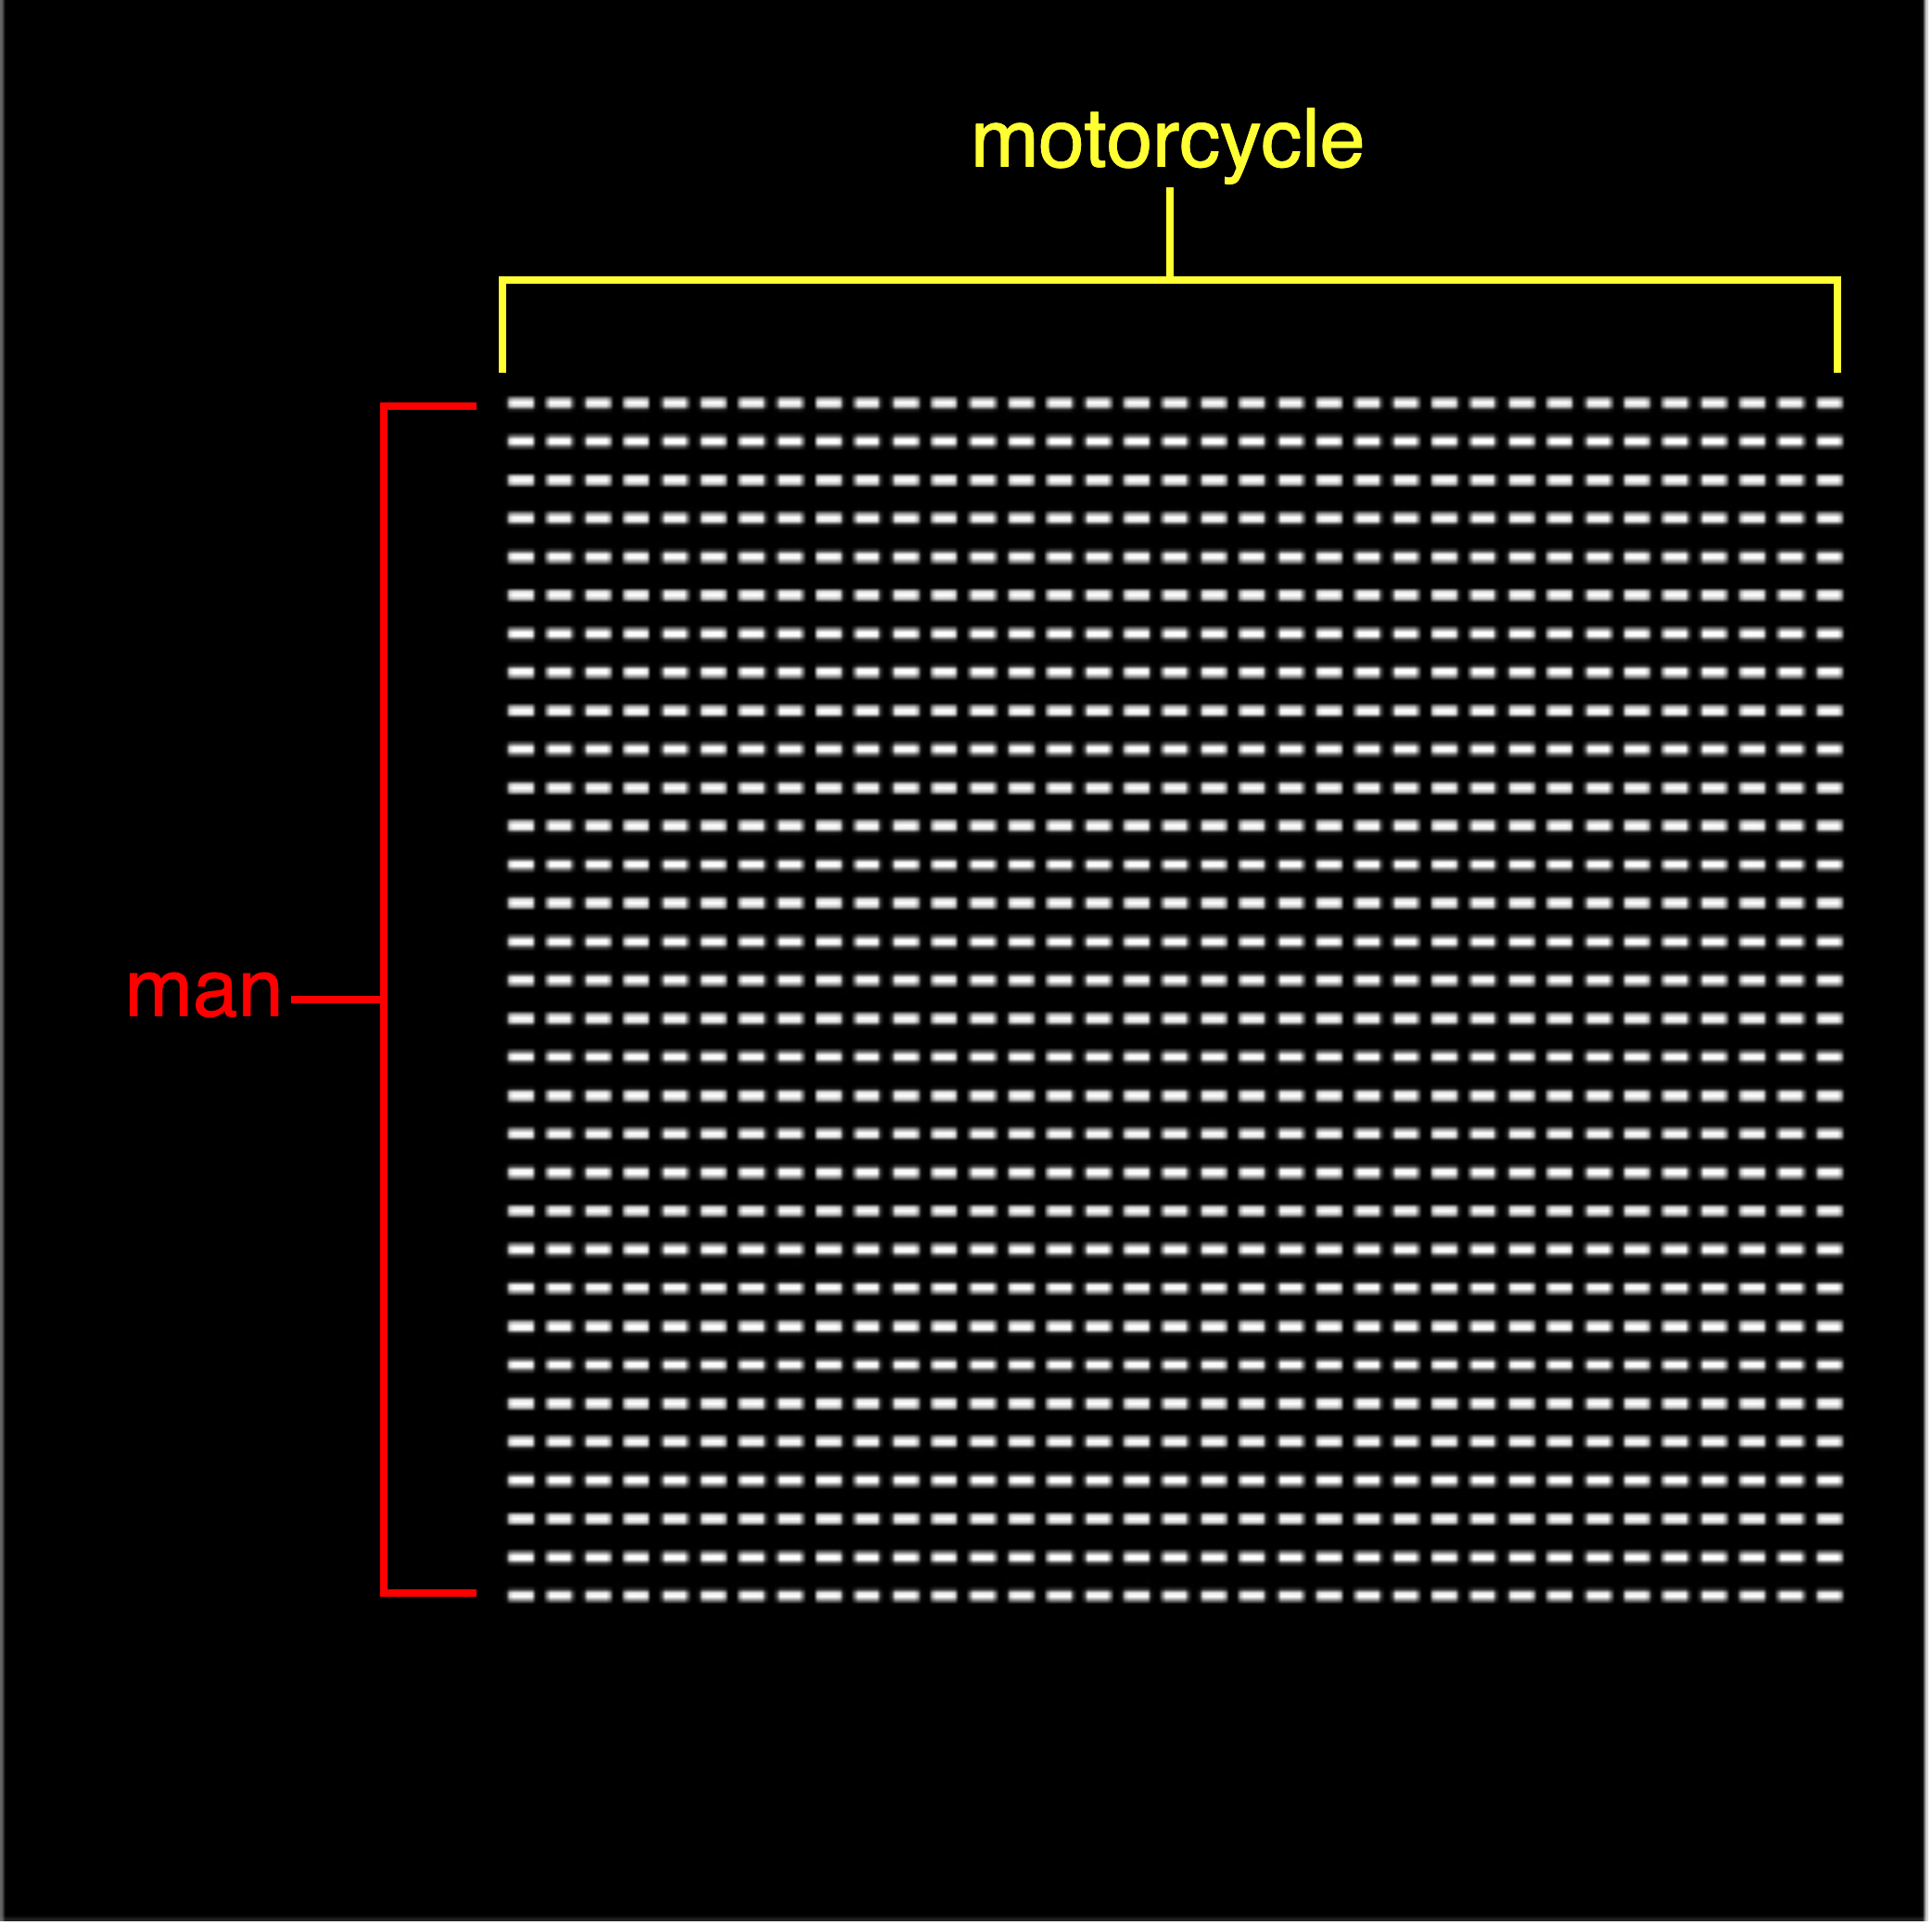
\includegraphics[width=0.9\linewidth]{figures/motor/map0}
			\label{fig:motor_map0}
	\end{minipage}}
	\subfigure[$\forall Attention_{p^i_{man} \to p^j_{wheel_1} } $]{
		\begin{minipage}[t]{5cm}
			\centering
			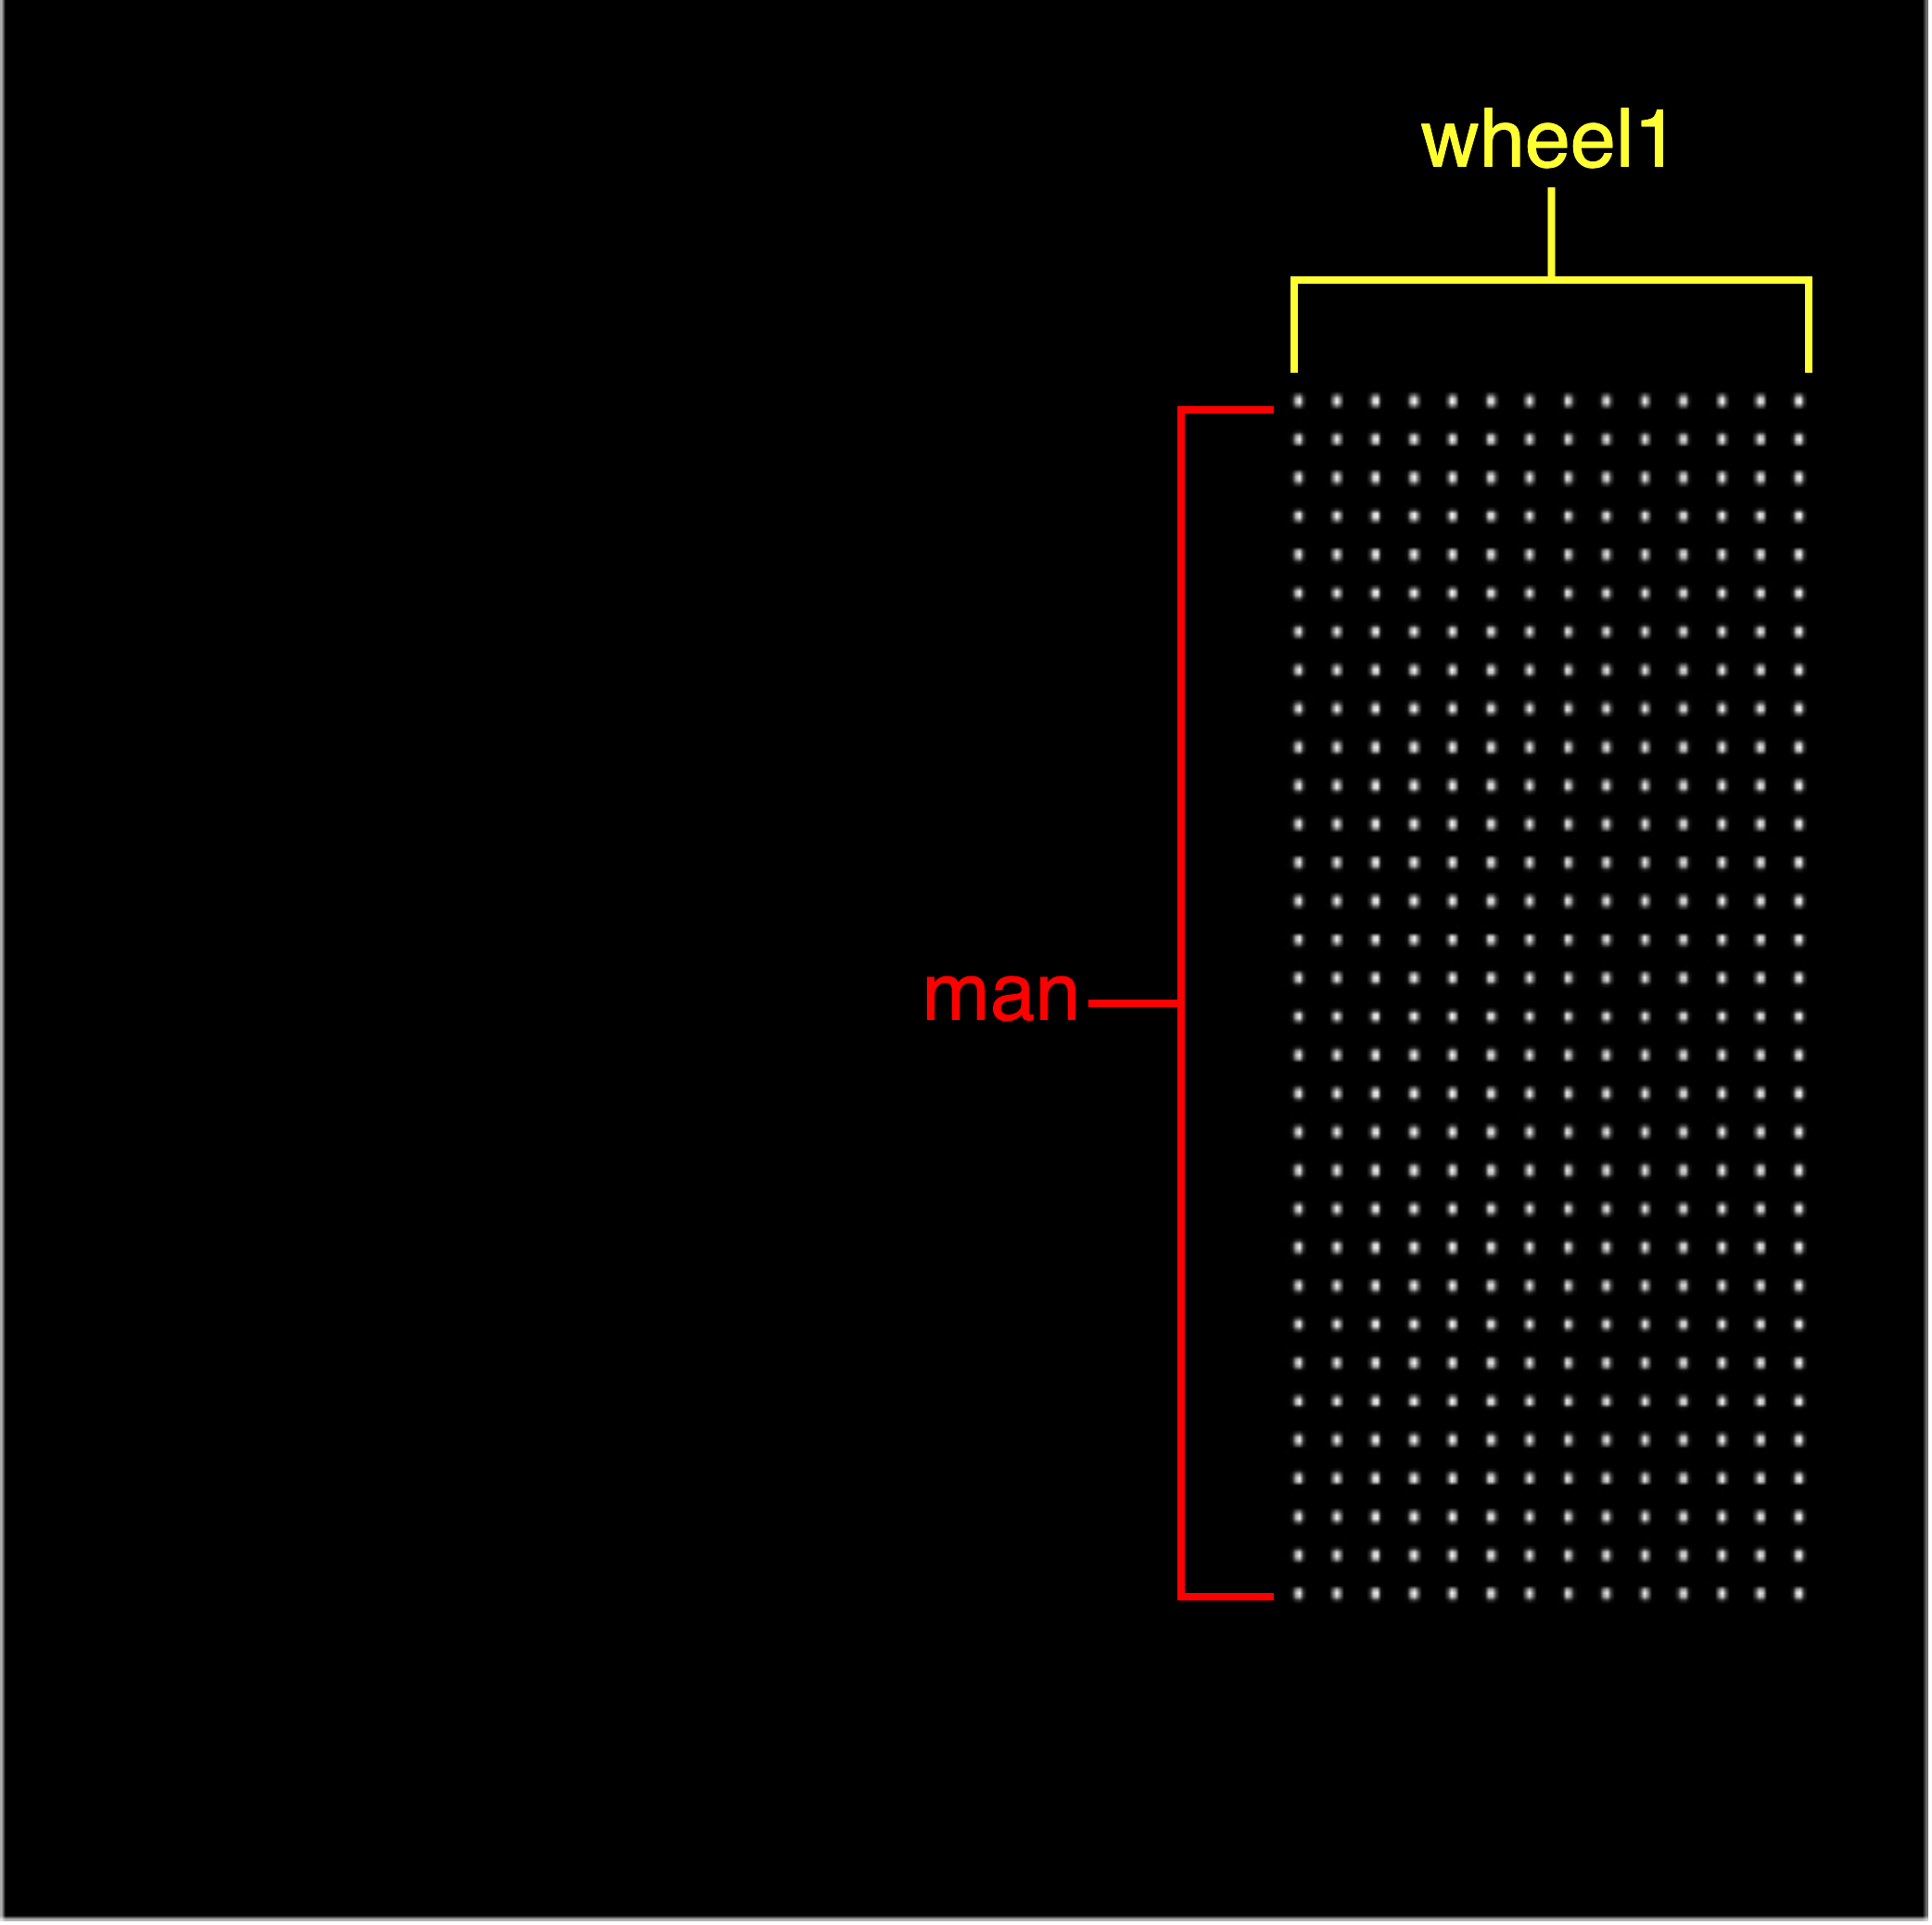
\includegraphics[width=0.9\linewidth]{figures/motor/map1}
			\label{fig:motor_map1}
	\end{minipage}}
	\subfigure[$\forall Attention_{p^i_{man} \to p^j_{wheel_2} } $]{
		\begin{minipage}[t]{5cm}
			\centering
			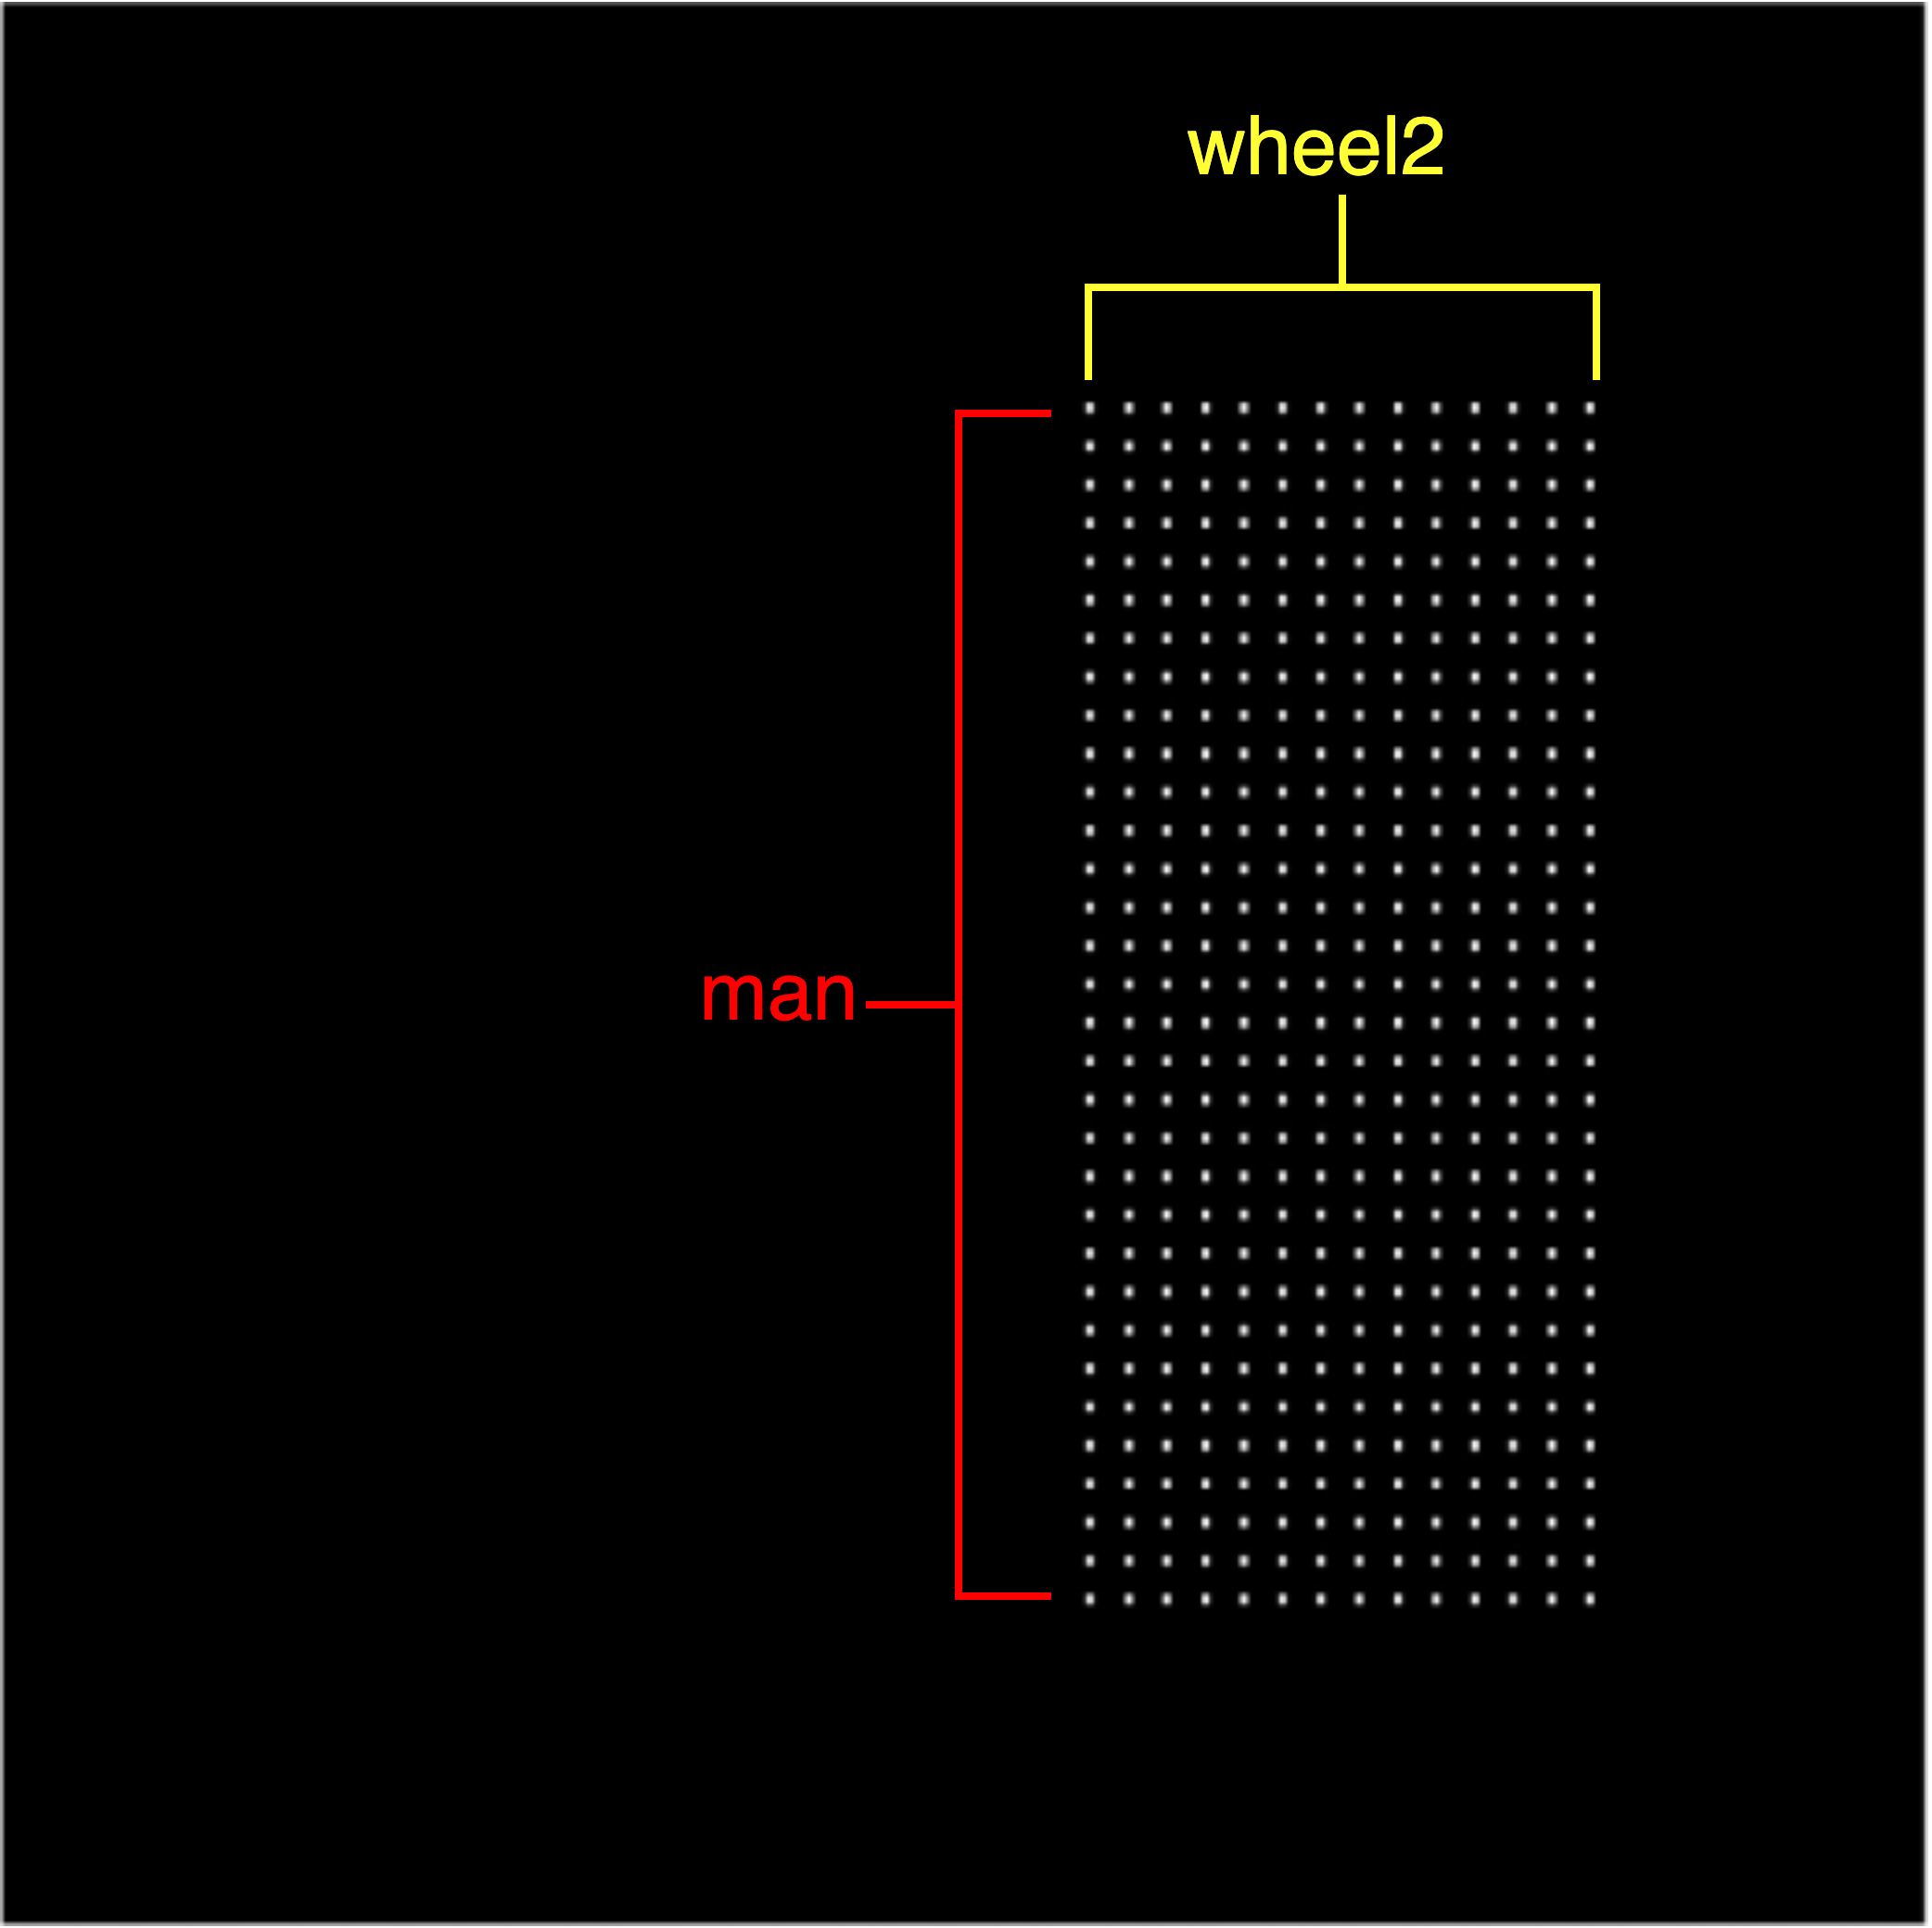
\includegraphics[width=0.9\linewidth]{figures/motor/map2}
			\label{fig:motor_map2}
	\end{minipage}}
	
	\caption[The attention map of each pair.]{The attention map of each pair, where $ (a) $ is the ground truth pair and $ (d) $ is its corresponding position in the attention map. $ (b) $, $(c) $ are no relationship pair, and $ (e) $, $ (f) $ is theirs corresponding positions in the attention map.}
	\label{fig:motor_pair}
\end{figure}

\begin{figure}[tbph!]
	\centering
	\subfigure[ $\forall Att^i_{rel}$]{
		\begin{minipage}[t]{5cm}
			\centering
			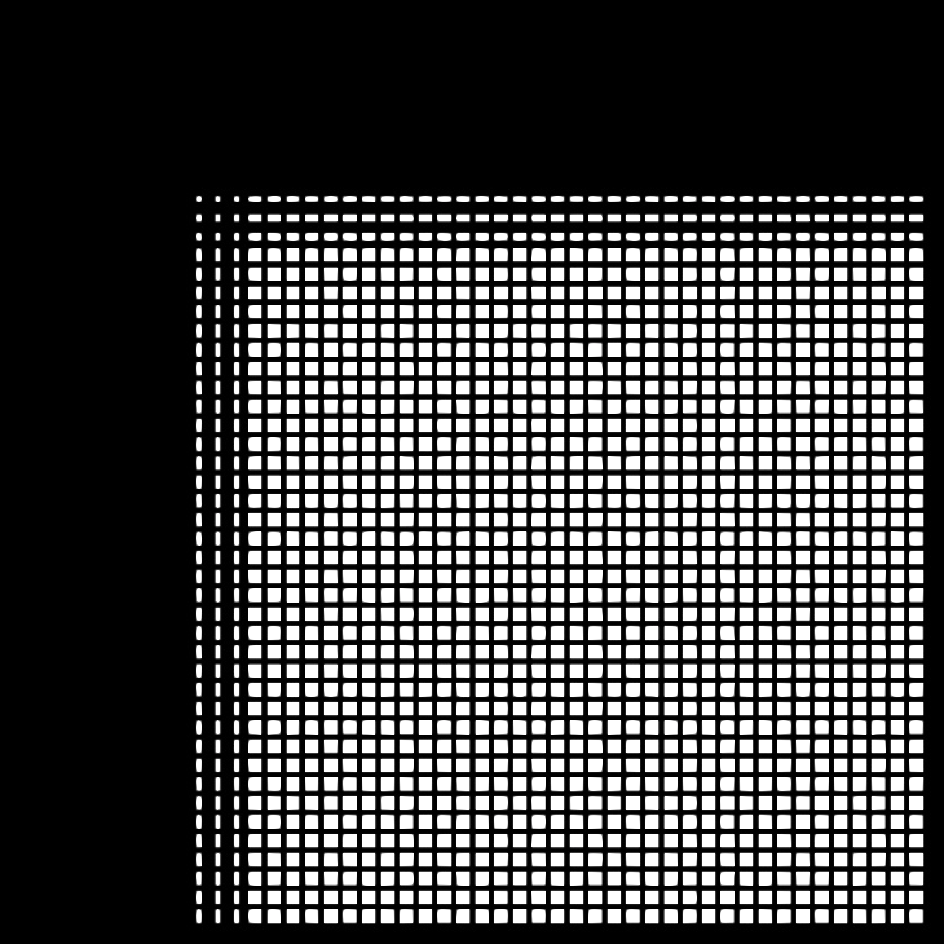
\includegraphics[width=0.9\linewidth]{figures/motor/all0}
			\label{fig:motor_all0}
	\end{minipage}}
	\subfigure[$ \forall Att^i_{no\_rel }$]{
		\begin{minipage}[t]{5cm}
			\centering
			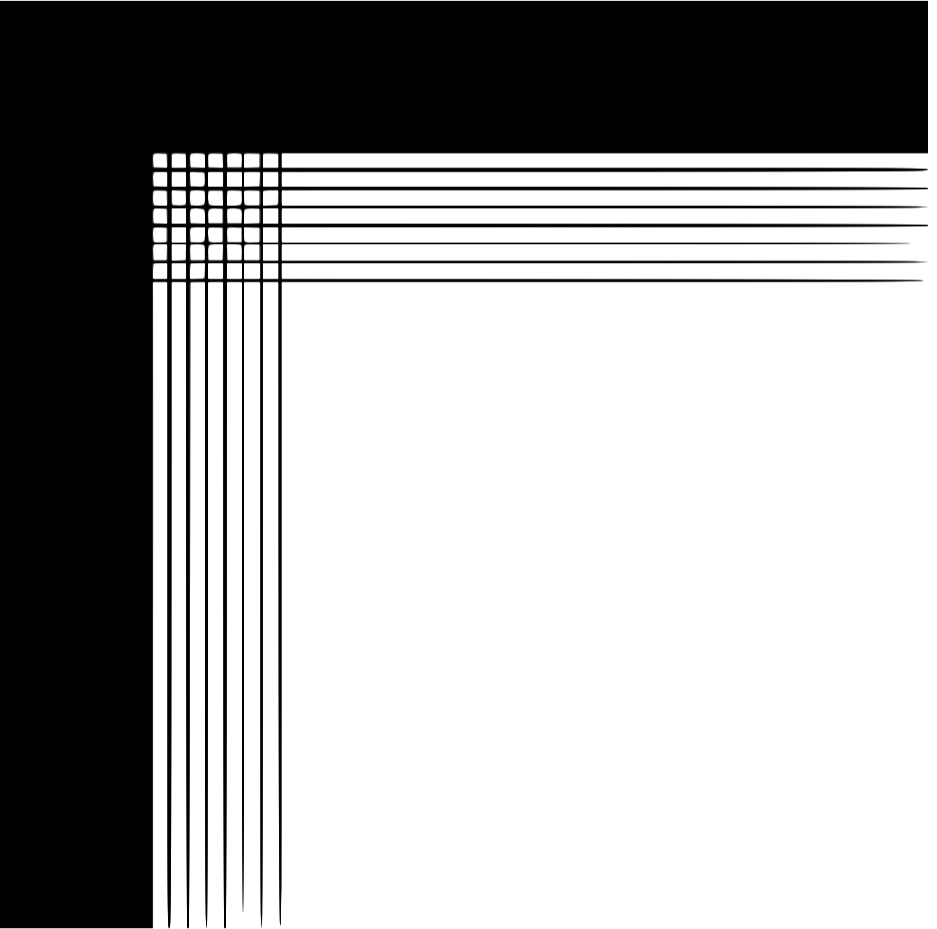
\includegraphics[width=0.9\linewidth]{figures/motor/all1}
			\label{fig:motor_all1}
	\end{minipage}}
	\subfigure[$ \forall Att^i_{rel} \cap  \forall Att^i_{no\_rel } $]{
		\begin{minipage}[t]{5cm}
			\centering
			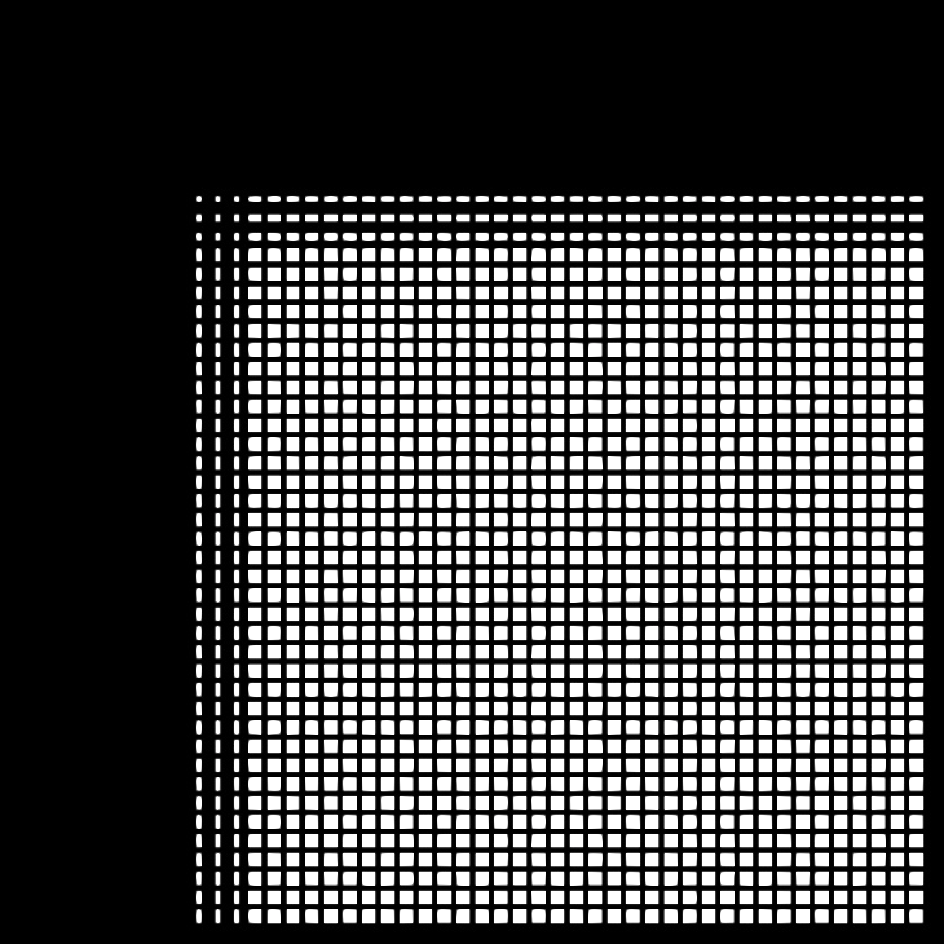
\includegraphics[width=0.9\linewidth]{figures/motor/all0}
			\label{fig:motor_all2}
	\end{minipage}}
	
	\caption[The overlap in Attention map]{The overlap in Attention map.The sub-figure (a) is the attention of all the related pairs, and the sub-figure (b) is the attention of all the irrelevant pairs. The sub-figure(c) shows that there is a serious overlap between them. We cannot increase the attention shown in (a) and decrease the attention of (b) through our attention loss.}
	\label{fig:overlap}
\end{figure}



\section{Experiments on Proposed Framework}

As mentioned above, our Pixel-based Attention idea was not able to meet our expectations due to the overlap, so we modified the model and designed Retina net.  
In this section, we introduce in detail the relevant experiments and results of Retina Net, including experiments on box query, attention map, relation decoder, as well as the parameter adjustment of the transformer, and the final result comparison.

\subsection{Implementation details}
 The model is implemented in $ pythorch\-0.4 $~\cite{paszke2019pytorch}. The input of the model is the same as Motifs-Net~\cite{zellers2018neural} , that is an image with a size of $ 592 \times 592 $. VGG16~\cite{simonyan2015deep} backbone pretrains the Visual Genome~\cite{krishna2017visual} dataset. As mentioned in  Sec.~\ref{sec:retinanet}, the encoder and the two decoder modules accept input features of size 2048. There are 3x Encoder, 3x Object Decoder , 3x Relation Decoder and 8 attention heads for transformer network. The GloVe vector embedding has size 200. SGD with momentum along with learning rate of $ 10^{-3 }$ and the batch size is 6. And cross-entropy loss function is adopted to compute the object and relation classification loss.

 We have followed three standard evaluation modes same as in current benchmark of the Motifs-Net~\cite{zellers2018neural} : (1) \textbf{predicate classification} (PredCLS): given a ground truth set of boxes and labels, predict relationship labels, (2) \textbf{scene graph classification} (SGCLS): given ground truth boxes, predict box labels and relationship label and (3) \textbf{scene graph detection} (SGDET): predict boxes, box labels, and relationship labels.
%For the  SGDET, we use a learnable object query, and use the Hungarian matching algorithm to match each object feature. For the other two subtasks\textbf{(setting)}, we use our custom object query to obtain the object feature.


\subsection{Experiment on Object Decoder}

The feasibility of our proposed object query to replace learnable query should be analyzed. The  PredCLS has classes and bounding boxes information, so we designed several object queries based on the known information, as shown in Fig.~\ref{fig:objectquery}, Fig.~\ref{fig:objquery1} and Fig.~\ref{fig:objquery2}. They are called  \textit{objec query 1} ,  \textit{objec query 2} , and  \textit{objec query 3}  respectively. Their pros and cons, and their substitutability are discussed  as follows.

The object query 1 mentioned in Sec.~\ref{sec:objectdecoder} has the spatial information of the entity, while the object query 2 is to add a class word embedding on its basis, so that our object query has semantic information. And object query 3 is obtained by a simple linear layer from the bounding box. Each entity in the picture has its own object query, because the object query depends on the bounding box.

\begin{figure}[tbph!]
	\centering
	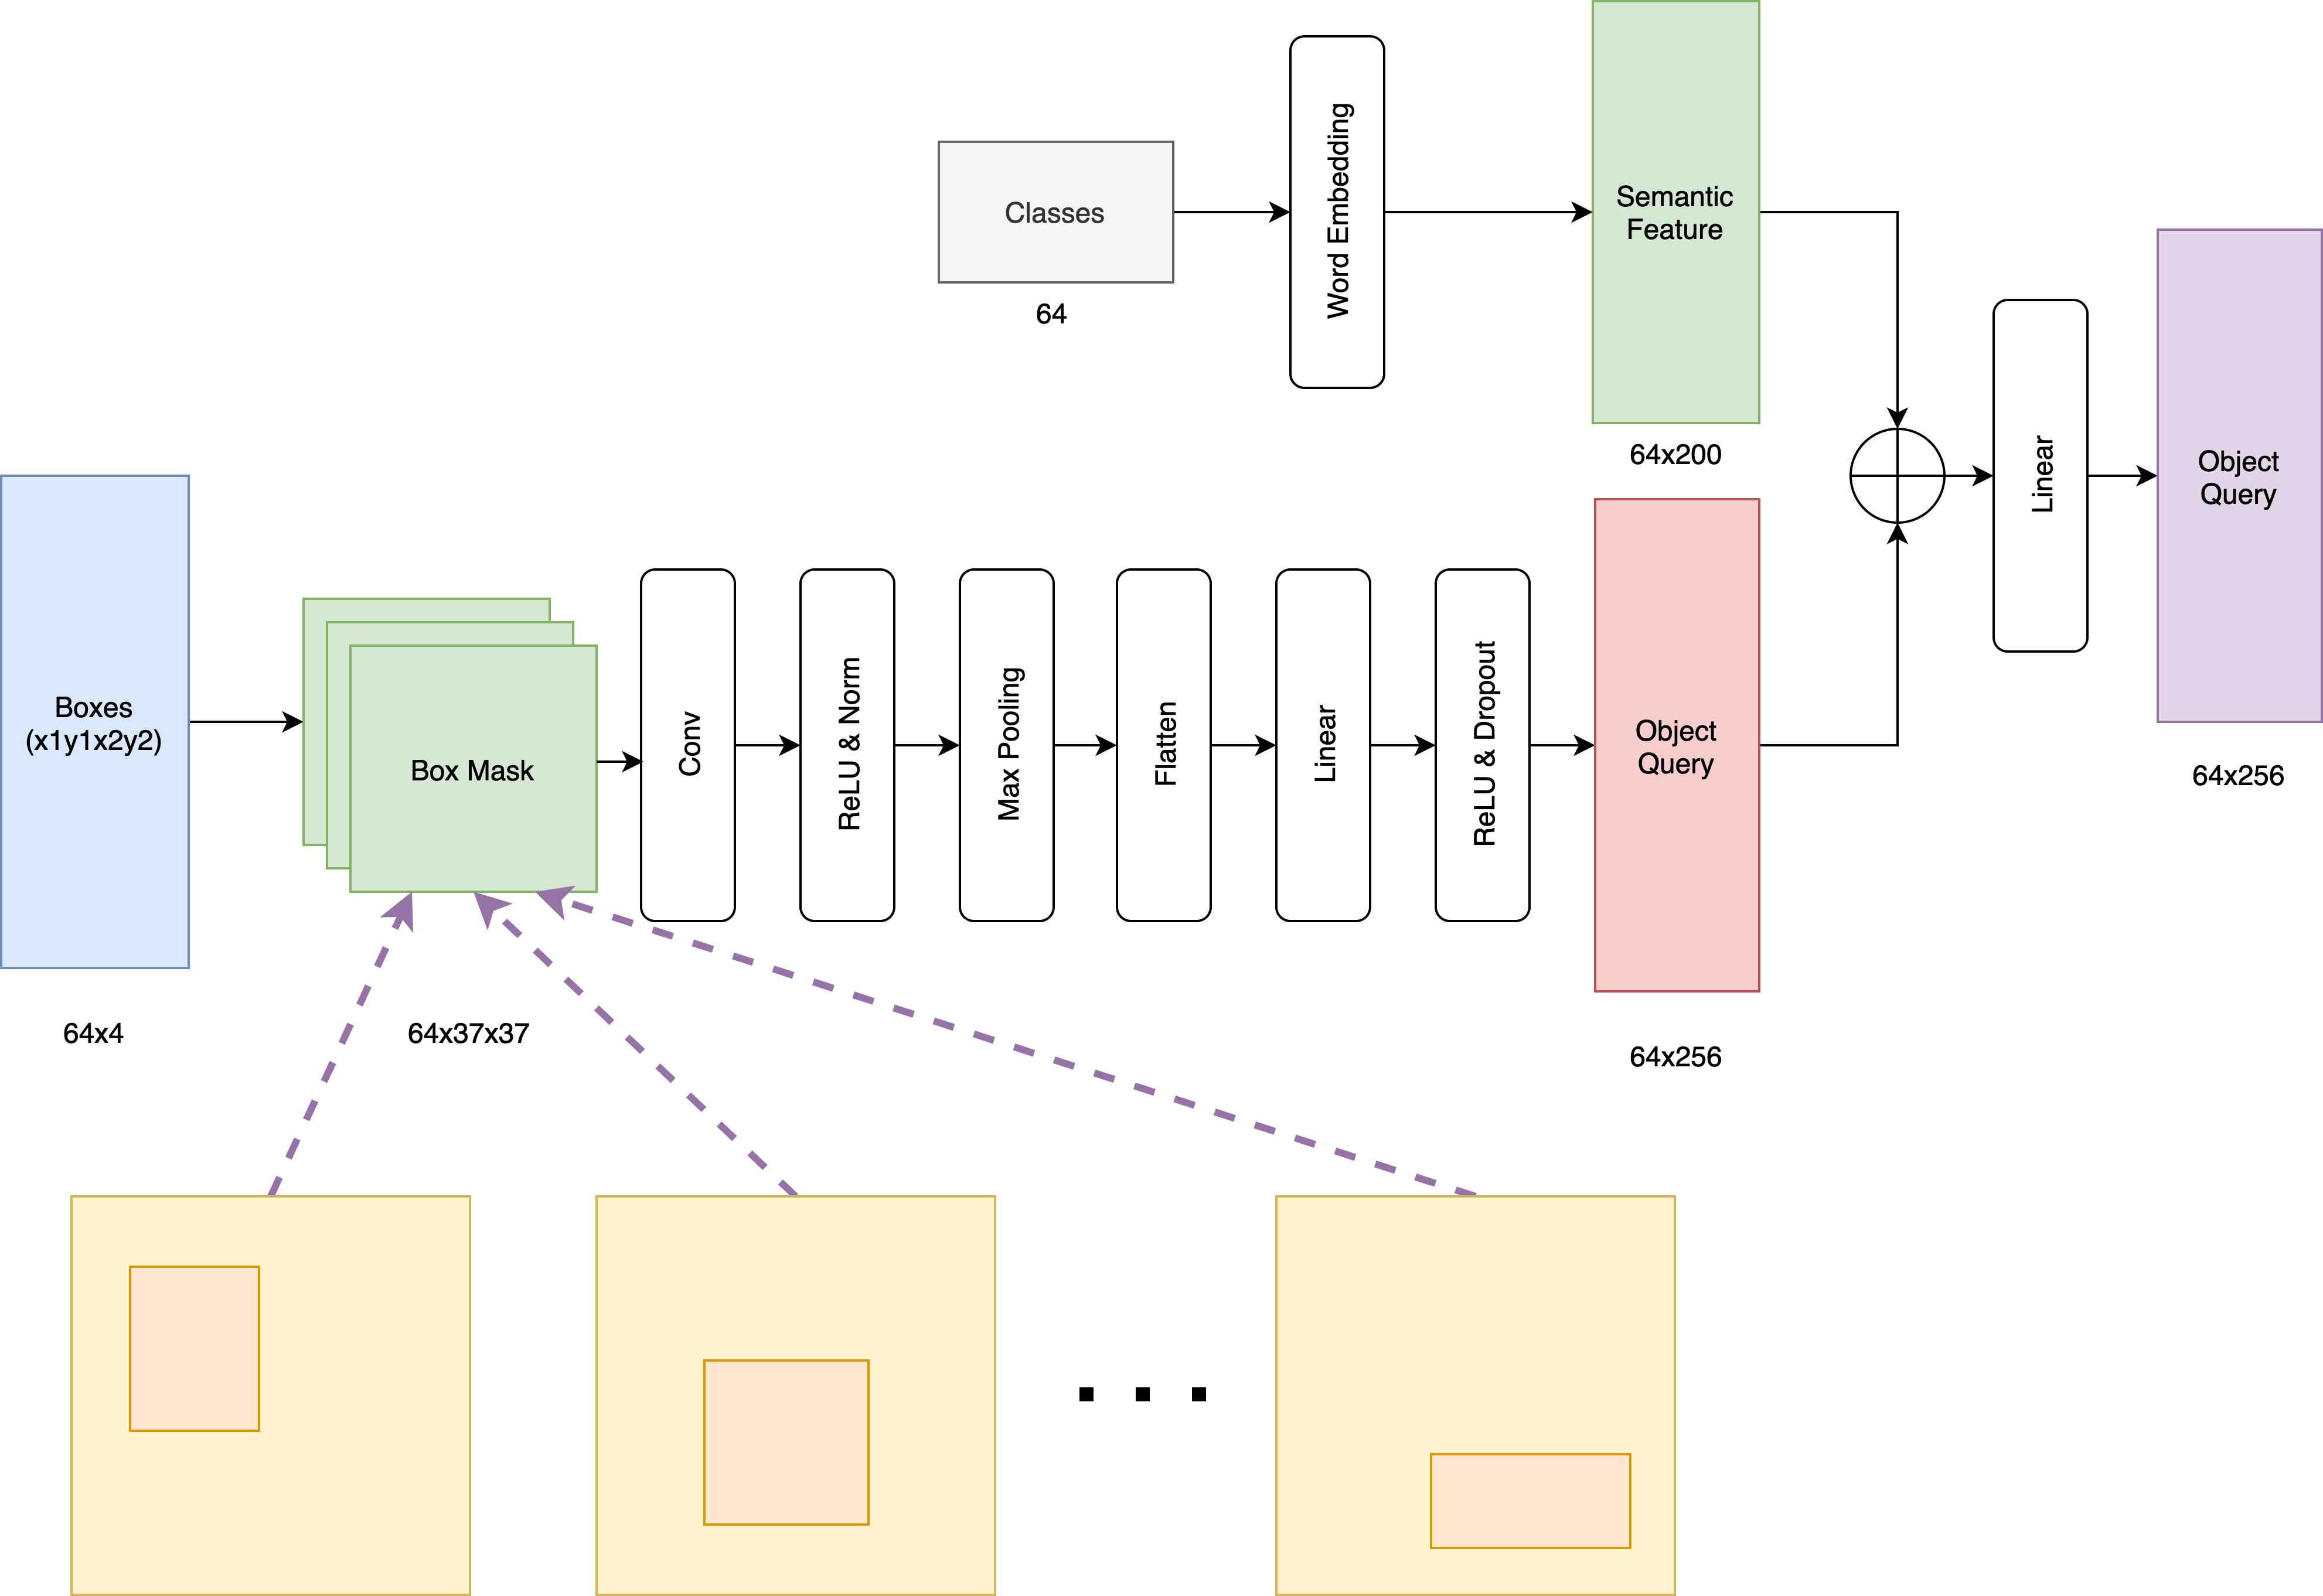
\includegraphics[width=0.8\linewidth]{figures/obj_query1}
	\caption[Illutrastion of the object query 2]{Illutrastion of the object query 2. Compared with object query1 in Fig.~\ref{fig:objquery1}, it integrate the semantic feature of objects.}
	\label{fig:objquery1}
\end{figure}

\begin{figure}[tbph!]
	\centering
	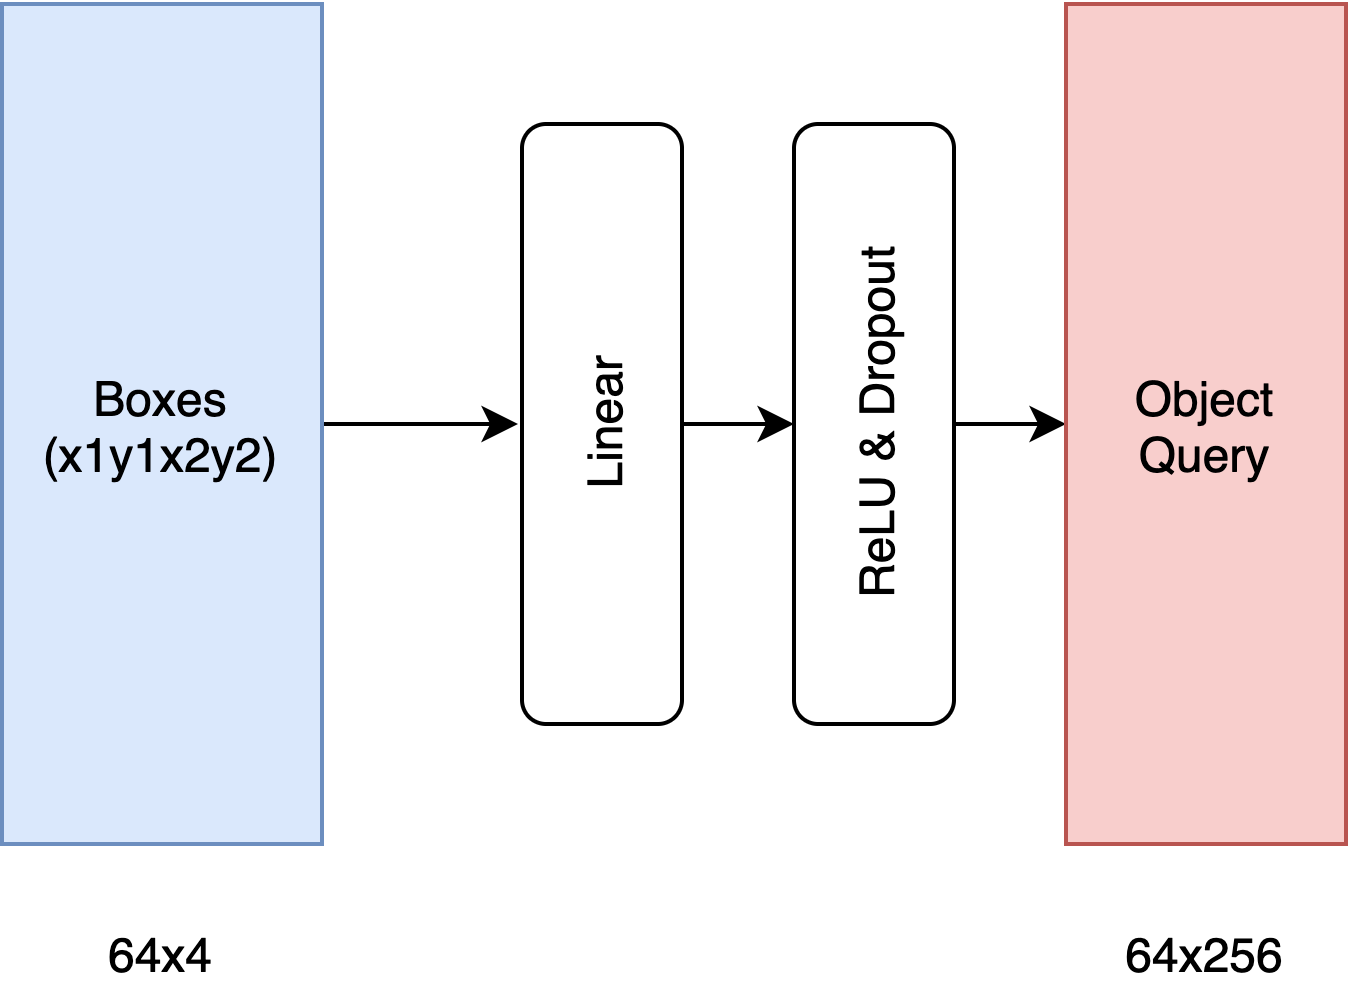
\includegraphics[width=0.5\linewidth]{figures/obj_query2}
	\caption[Illutrastion of the object query 3]{Illutrastion of the object query 3,we only added a simple linear layer behind the bounding box.}
	\label{fig:objquery2}
\end{figure}

\subsubsection{Consistency of the Object Query }

DETR uses a learnable embedding vector as the query,and it utilizes the Hungarian matching algorithm to find the most matching object feature, because their queries have no actual physical meaning, and the queries are fixed for each picture and cannot establish a direct connection with the actual object.%且对于每一张图片他都是固定的,无法与实际的object 建立直接的联系。
However,since our object query contains relevant information of each object, such as spatial information and semantic information, it is in one-to-one correspondence with the entities in the picture.

In order to verify the correspondence between the object query and the entity in the picture, a box regression is designed in the experiment. After the object query and object feaure, two Multilayer Perceptron(MLP) modules are separately added, and then observe whether they can regain the spatial information of the object.For the evaluation metrics, IoU and GIoU~\cite{rezatofighi2019generalized} are used .

After the MLP, a bounding box vector $ \hat{b_\sigma} $ is obtained, then the box loss $\mathcal{L}_{box}$can be calculated with ground truth bounding box $b$. The box loss consists of a GIoU loss $  \mathcal{L}_{GIoU} $ and a $l_1$ loss, see the following equation:

$$ \mathcal{L}_{box}(b,\hat{b}_{\hat{\sigma}}) = \mathcal{L}_{GIoU}(b,\hat{b}_{\sigma}) + \left \| b - \hat{b}_{\sigma}  \right \| _1 $$

\begin{table}[!h]
	\centering
	\begin{tabular}{c|ccc}
		\bottomrule
		& object query 1 & object query 2 & object query 3  \\ \midrule
		IoU  & 0.759  & 0.750  & 0.681    \\
		GIoU & 0.744  & 0.733 & 0.669   \\ \midrule
		&object feature 1  &object feaure 2 & object feautre 3\\ \midrule
		IoU & 0.634 & 0.631 & 0.580 \\
		GIoU	& 0.617 & 0.620 & 0.568  \\\bottomrule
		
	\end{tabular}
\caption[The regression result of the object query and feature]{The regression result of the object queries and features.}
\label{tab:regresstion}
\end{table}

Table~\ref{tab:regresstion} shows that the IoU of object queries can reach 0.75 and the IoU of object features averages 0.6. This verifies that there is a one-to-one correspondence between all three object queries and objects, and the object query 3 is slightly worse than the others.

\subsubsection{The comparison of object queries}
The object query is a $ 64 \times 256 $ matrix, corresponding to the objects in each image, so  each object query can be reshaped into a size of $16 \times 16$ image. Fig.~\ref{fig:tennis}  shows that three different queries are generated through three different methods, and the query corresponding to each object is also different. For example, in Figure(b), as the area of our entities gradually increases, the query gradually becomes denser. 


\begin{figure}[h!]
	\centering
	\subfigure[The objects with bounding boxes.]{
		\begin{minipage}[t]{3.5cm}
			\centering
			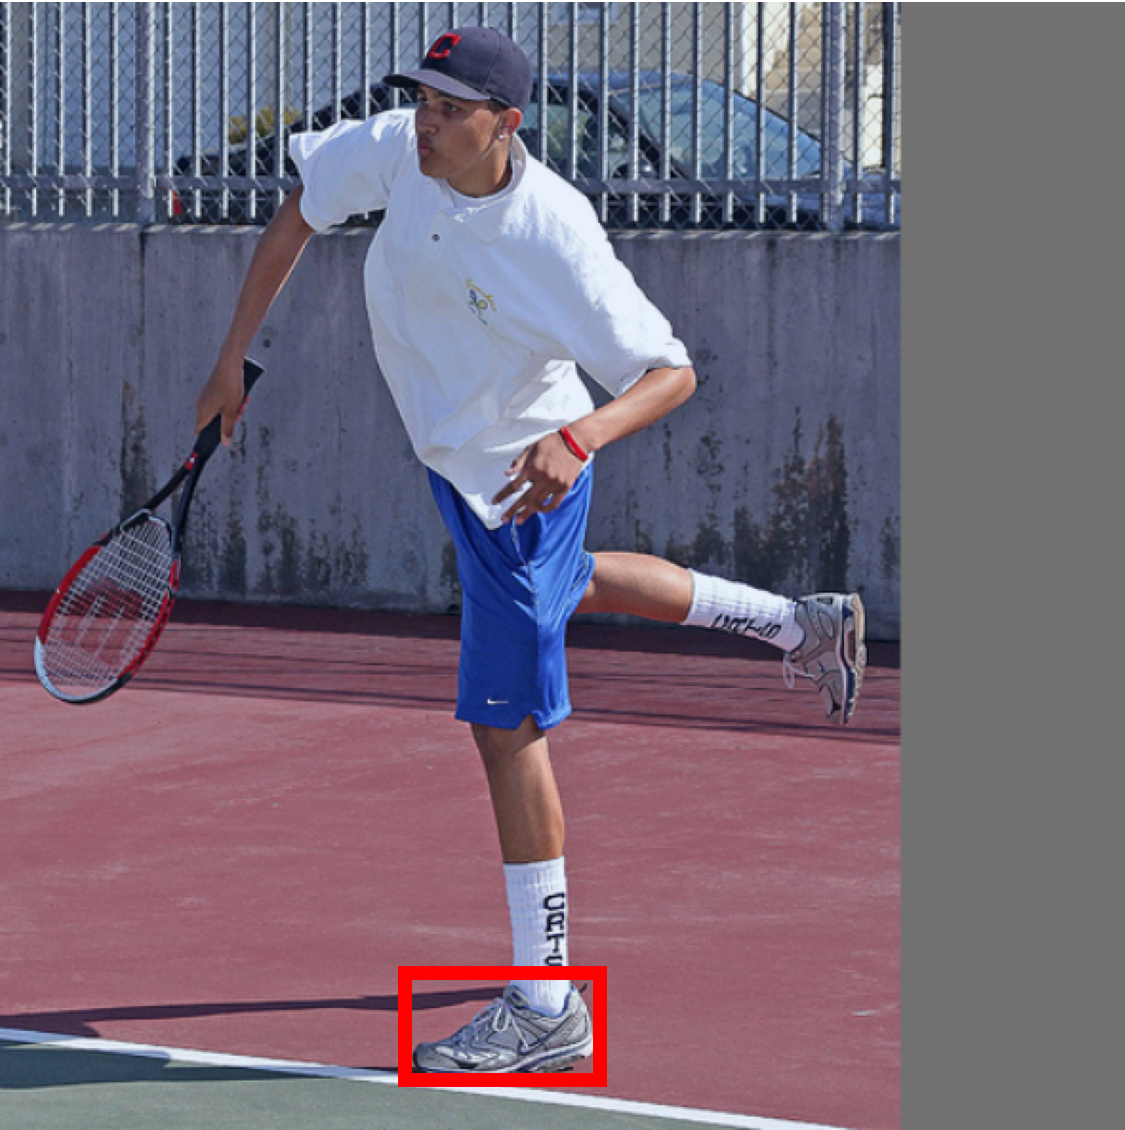
\includegraphics[width=0.9\linewidth]{figures/result/tennis/obj2}
	\end{minipage}
		\begin{minipage}[t]{3.5cm}
			\centering
			\includegraphics[width=0.9\linewidth]{figures/result/tennis/obj4}
	\end{minipage}
	\begin{minipage}[t]{3.5cm}
		\centering
		\includegraphics[width=0.9\linewidth]{figures/result/street/o3}
	\end{minipage}
		\begin{minipage}[t]{3.5cm}
			\centering
			\includegraphics[width=0.9\linewidth]{figures/result/street/o4}
	\end{minipage}}
	
	\subfigure[The object query 1.]{
		\begin{minipage}[t]{3.5cm}
			\centering
			\includegraphics[width=0.9\linewidth]{figures/result/tennis/q0_2}
	\end{minipage}
		\begin{minipage}[t]{3.5cm}
			\centering
			\includegraphics[width=0.9\linewidth]{figures/result/tennis/q0_4}
	\end{minipage}
	\begin{minipage}[t]{3.5cm}
		\centering
		\includegraphics[width=0.9\linewidth]{figures/result/street/q0_3}
	\end{minipage}
		\begin{minipage}[t]{3.5cm}
			\centering
			\includegraphics[width=0.9\linewidth]{figures/result/street/q0_4}
	\end{minipage}}


		\subfigure[the object query 2.]{
		\begin{minipage}[t]{3.5cm}
			\centering
			\includegraphics[width=0.9\linewidth]{figures/result/tennis/q3_2}
	\end{minipage}
		\begin{minipage}[t]{3.5cm}
			\centering
			\includegraphics[width=0.9\linewidth]{figures/result/tennis/q3_4}
	\end{minipage}
		\begin{minipage}[t]{3.5cm}
			\centering
			\includegraphics[width=0.9\linewidth]{figures/result/street/q3_3}
	\end{minipage}
		\begin{minipage}[t]{3.5cm}
			\centering
			\includegraphics[width=0.9\linewidth]{figures/result/street/q3_4}
	\end{minipage}}

	\subfigure[The object query 3.]{
		\begin{minipage}[t]{3.5cm}
			\centering
			\includegraphics[width=0.9\linewidth]{figures/result/tennis/q2_2}
	\end{minipage}
		\begin{minipage}[t]{3.5cm}
			\centering
			\includegraphics[width=0.9\linewidth]{figures/result/tennis/q2_4}
	\end{minipage}
	\begin{minipage}[t]{3.5cm}
	\centering
	\includegraphics[width=0.9\linewidth]{figures/result/street/q2_3}
	\end{minipage}
	\begin{minipage}[t]{3.5cm}
	\centering
	\includegraphics[width=0.9\linewidth]{figures/result/street/q2_4}
	\end{minipage}}

	\caption[An instance of Visualized results of the object query]{An instance of visualized results of the object query. From top to bottom, each row represents the position of the object, object query 1, object query 2 and object query 3.}
	\label{fig:tennis}
\end{figure}

 % 不同的object query的效果
Next, the object queries are fed into the object decoder to test their performance in the PredCLS, and recall@50 and recall@100 as the evaluation metrics. The results are in Table~\ref{tab:result_object _query}.

\begin{table}[!h]
	\centering
	\begin{tabular}{c|ccc}
		\hline
		& object query 1 & object query 2 & object query 2 \\ \hline
		Recall@50  & 62.9            & 63.2            & 63.0              \\
		Recall@100 & 65.0             & 65.3              & 65.1              \\ \hline
	\end{tabular}

\caption[The comparison of the object queries in PredCLS]{The comparison of the object queries in PredCLS.}
\label{tab:result_object _query}
\end{table}

According to the above table,  the conclusions as follows:

\begin{enumerate}
	\item The object query and object feature we designed correspond to each other, which can replace learnable query and solve the VRD problem.
	\item The performance of the three object queries in PredCLS is similar. So it only need to design a query that can distinguish objects, that is, each query needs to correspond to a unique entity. 
\end{enumerate}

\subsubsection{Experiment on Object Context}
In order to obtain more information that is conducive to predicate prediction, the object context is designed to obtain the interaction between objects. It contains a global context of an object to all objects. Predicate prediction itself is to detect the interaction between objects, so a context that can indicate the interaction information between them is very necessary. Remove $ context_{obj }$ in the predicate classifier and compare the formula ~\ref{equ:predicatd}  and ~\ref{equ:predicatc} to detect the effect of object context on Predicate Classification.
% 为了获取更多有利于谓语预测的信息,我们设计了object context,去获得object 之间的交互,它包含了一个object 对所有object的上下文关系。谓语预测本身就是检测object间的交互,所以一个能表明他们之间的交互信息的context是十分必要的。在predicate classifier中去掉 $ context_{obj }$ 使用如下公式~\ref{equ:predicatd}与公式~\ref{equ:predicatc}进行对比,检测object  context 对Predicate Classification的作用效果。

\begin{equation}
	score'_{pred}(i,j) = Linear(concat(feat_{obj}^i, context_{rel}^{ij}, feat_{obj}^j)
	\label{equ:predicatd}
\end{equation}

\begin{table}[]
	\begin{tabular}{llll}
		\hline
		a & sd & dw  & asd \\ \hline
		3 & 12 & 231 & 12  \\ \hline
	\end{tabular}
\end{table}

\begin{table}[]
	\centering
	\begin{tabular}{c|lcc}
		\hline
		\multirow{2}{*}{}      & \multicolumn{3}{l}{Predicate Classification}  \\ \cline{2-4} 
		& R@20          & R@50          & R@100         \\ \hline
		without object context & 51.7          & 59.6          & 62.3          \\
		with object context    & \textbf{55.4} & \textbf{63.4} & \textbf{64.4} \\ \hline
	\end{tabular}
\caption[The impact of object context on PredCLS]{The impact of object context on PredCLS.}
\label{tab:object context}
\end{table}
As shown in Table~\ref{tab:object context}, the object context has great benefits for the predicate prediction, especially the improvement of recall@20 is the most obvious, with an improvement of 3.7. This verifies the effect of global context between objects on predicate prediction.% 通过上表,可是肯定object context 对谓语预测的有很大帮助,尤其是recall@20的提高最为明显,有3.7的提升。这验证的global context between objects 对谓语预测的作用。

\subsection{Experiment on Attention  Loss Function}

An attention loss is designed to make the object feature better and some experiments are performed to verify it.

The Figure~\ref{fig:attention_loss_result} is the training result of the attention loss. We record a loss every 100 steps, summing up 1000 data, and use Matlab to perform low-pass filtering to draw the result. It is showed that the attention from the beginning $ 10^{-4} $ dropped rapidly and gradually tended to 0 after 500 steps.

In the object decoder in our model in Fig.~\ref{fig:objectdecoder}, when the feature of the object is obtained, it will be accompanied by the corresponding attention map. Its size is $ 64\times1369 $, corresponding to each object, it is reshaped into a size of $ 37\times37 $ object attention map. As shown in Fig.~\ref{fig:train_attention_loss} and Fig.~\ref{fig:bus}. The first and second image are selected in our test data set, and the object bounding boxes and their attention maps (with and without attention loss) are drawn.

\begin{figure}[H]
	\centering
	\includegraphics[width=0.7\linewidth]{figures/result/attention_loss}
	\caption[Training result of the Attention Loss]{Training result of the Attention Loss.}
	\label{fig:attention_loss_result}
\end{figure}

It can be seen that the attention loss performs successfully on the attention map. Without attention loss, the attention map is messy. As shown in Fig.~\ref{fig:train_attention_loss}(b), the position and shape of the train can be distinguished well in the attention map, and it even express the position of the train better than the bounding box. The background area of the picture is blue, and the background color in the picture is very uniform, which makes the attention weight of the object very obvious. It means the object decoder pays more attention to this object.

\begin{figure}[H]
	\centering
	\subfigure[train]{
		\begin{minipage}[t]{5cm}
			\centering
			\includegraphics[width=0.9\linewidth]{figures/result/train/obj1}
	\end{minipage}}
	\subfigure[attention map with our loss]{
		\begin{minipage}[t]{5cm}
			\centering
			\includegraphics[width=0.9\linewidth]{figures/result/train/att1}
	\end{minipage}}
	\subfigure[ attention map without our loss]{
		\begin{minipage}[t]{5cm}
			\centering
			\includegraphics[width=0.9\linewidth]{figures/result/train/no1}
	\end{minipage}}
	
	\subfigure[haus]{
		\begin{minipage}[t]{5cm}
			\centering
			\includegraphics[width=0.9\linewidth]{figures/result/train/obj2}
	\end{minipage}}
	\subfigure[attention map with our loss]{
		\begin{minipage}[t]{5cm}
			\centering
			\includegraphics[width=0.9\linewidth]{figures/result/train/att2}
	\end{minipage}}
	\subfigure[attention map without our loss]{
		\begin{minipage}[t]{5cm}
			\centering
			\includegraphics[width=0.9\linewidth]{figures/result/train/no2}
	\end{minipage}}
	
	\subfigure[man]{
		\begin{minipage}[t]{5cm}
			\centering
			\includegraphics[width=0.9\linewidth]{figures/result/train/obj3}
	\end{minipage}}
	\subfigure[attention map with our loss]{
		\begin{minipage}[t]{5cm}
			\centering
			\includegraphics[width=0.9\linewidth]{figures/result/train/att3}
	\end{minipage}}
	\subfigure[attention map without our loss]{
		\begin{minipage}[t]{5cm}
			\centering
			\includegraphics[width=0.9\linewidth]{figures/result/train/no3}
	\end{minipage}}
	
	\subfigure[window]{
		\begin{minipage}[t]{5cm}
			\centering
			\includegraphics[width=0.9\linewidth]{figures/result/train/obj4}
	\end{minipage}}
	\subfigure[attention map with our  loss]{
		\begin{minipage}[t]{5cm}
			\centering
			\includegraphics[width=0.9\linewidth]{figures/result/train/att4}
	\end{minipage}}
	\subfigure[attention map without our loss]{
		\begin{minipage}[t]{5cm}
			\centering
			\includegraphics[width=0.9\linewidth]{figures/result/train/no4}
	\end{minipage}}
	
	\caption[The visualization of our attention loss of the first image in the test dataset]{The visualization of our attention loss of the first image in the test dataset. The first column is the object bounding box, the second column is the visualization result of the attention map when we use the attention loss, and the third column is the visualization result of the attention map without our attention loss.}
	\label{fig:train_attention_loss}
\end{figure}




\begin{figure}[H]
	\centering
	\subfigure[bus]{
		\begin{minipage}[t]{5cm}
			\centering
			\includegraphics[width=0.9\linewidth]{figures/result/bus/obj1}
	\end{minipage}}
	\subfigure[attention map with our loss]{
		\begin{minipage}[t]{5cm}
			\centering
			\includegraphics[width=0.9\linewidth]{figures/result/bus/att1}
	\end{minipage}}
	\subfigure[attention map without our loss]{
		\begin{minipage}[t]{5cm}
			\centering
			\includegraphics[width=0.9\linewidth]{figures/result/bus/no1}
	\end{minipage}}
	
	\subfigure[man]{
		\begin{minipage}[t]{5cm}
			\centering
			\includegraphics[width=0.9\linewidth]{figures/result/bus/obj2}
	\end{minipage}}
	\subfigure[attention map with our loss]{
		\begin{minipage}[t]{5cm}
			\centering
			\includegraphics[width=0.9\linewidth]{figures/result/bus/att2}
	\end{minipage}}
	\subfigure[attention map without our loss]{
		\begin{minipage}[t]{5cm}
			\centering
			\includegraphics[width=0.9\linewidth]{figures/result/bus/no2}
	\end{minipage}}
	
	\subfigure[pants]{
		\begin{minipage}[t]{5cm}
			\centering
			\includegraphics[width=0.9\linewidth]{figures/result/bus/obj3}
	\end{minipage}}
	\subfigure[ attention map with our loss]{
		\begin{minipage}[t]{5cm}
			\centering
			\includegraphics[width=0.9\linewidth]{figures/result/bus/att3}
	\end{minipage}}
	\subfigure[ attention map without our loss]{
		\begin{minipage}[t]{5cm}
			\centering
			\includegraphics[width=0.9\linewidth]{figures/result/bus/no3}
	\end{minipage}}
	
	\subfigure[board]{
		\begin{minipage}[t]{5cm}
			\centering
			\includegraphics[width=0.9\linewidth]{figures/result/bus/obj4}
	\end{minipage}}
	\subfigure[ attention map with our loss]{
		\begin{minipage}[t]{5cm}
			\centering
			\includegraphics[width=0.9\linewidth]{figures/result/bus/att4}
	\end{minipage}}
	\subfigure[ attention map without our loss]{
		\begin{minipage}[t]{5cm}
			\centering
			\includegraphics[width=0.9\linewidth]{figures/result/bus/no4}
	\end{minipage}}
	
	\caption[The visualization of our attention loss of the second image in the test dataset]{The visualization of our attention loss of the second image in the test dataset. The first column is the object bounding box, the second column is the visualization result of the attention map when we use the attention loss, and the third column is the visualization result of the attention map without our attention loss.}
	\label{fig:bus}
\end{figure}


\begin{table}[!h]
	\centering
	\begin{tabular}{c|ccc|ccc}
		\hline
		\multirow{2}{*}{}           & \multicolumn{3}{c|}{PredCLS} & \multicolumn{3}{c}{SGCLS} \\ \cline{2-7} 
		& R@20    & R@50    & R@100    & R@20   & R@50   & R@100   \\ \hline
		without our attention  loss & 53.9      & 61.8       & 64.0       & 25.7     & 30.7     & 31.4   \\
		with our attention loss     & \textbf{55.4}       & \textbf{63.3}       & \textbf{65.2 }       & \textbf{28.4 }     & \textbf{32.7}      &\textbf{33.6}     \\ \hline
	\end{tabular}
	
	\caption[The result of attention loss in PredCLS and SGCLS]{The result of attention loss in PredCLS and SGCLS.}
	\label{tab:result_attetnion_loss}
\end{table}


According to Table~\ref{tab:result_attetnion_loss}, in PredCLS R@50 has an improvement of about 0.1, and in SGCLS it is even greater by about 0.2.

Based on the above results, the conclusion is as follows  :
\begin{enumerate}
	\item Our attention loss can effectively change the attention map so that it can be well visualized and can show the position and shape of each object.
	\item Our attention loss can get a better object feature, so as to better solve the VRD problem.
\end{enumerate}

\subsection{Experiment on Relation Deocder}
In this section,  experiments on the relation decoder are conducted. Based on the results of the previous object query, a different relation query is designed, and it makes our relation context have the spatial information and semantic information of the object.

%In Figure~\ref{fig:relation_d_vis}, we can see that the relationship query we designed has differences between each relationship pair. For example, in the figure (a) represents pair $ <man, pants?>$ and (b) represents pair $ <pant, man> $, their subject and The objects are opposite, but their relations are different. In the figure (c) is relation pair $ <man1, glove> $ and d is $ <man1, man2> $. They have the same subject and different objects, but their relation queries are also significantly different.

In Figure~\ref{fig:relation_attetnion}, the context effect is expressed through attention between relation and object. When the relational context is obtained through the relational decoder, it will be accompanied by an attention map. The sub-figure(c) and (f) are attention map, which y-axis represents the relation pair and its x-axis represents the object. Our relation pair contains both ground truth pair and no relation pair. For example, in sub-figure(a), the ground truth pair $<glass, table> $ has higher attention weight for object \textit{`glass'} and \textit{`table'} than others, which means that this pair pays more attention to the objects \textit{`glass'} and \textit{`table'}. No relation pair has the same effect. For example, in the attention map on the right,the attention values of the object \textit{ `hair'} and \textit{`glove'} in the pair $<hair, glove> $   is higher than the object \textit{`girl'}.


\begin{figure}[!htp]
	\centering
	\subfigure[Scene graph]{
		\begin{minipage}[t]{5cm}
			\centering
			\includegraphics[width=0.7\linewidth]{figures/result/relation_Attention/img1}
		\end{minipage}}
	\subfigure[Ground truth relationships ]{
		\begin{minipage}[t]{5cm}
			\centering
			\includegraphics[width=0.8\linewidth]{figures/result/relation_Attention/rel1}
		\end{minipage}}
	\subfigure[Attention map]{
		\begin{minipage}[t]{5cm}
			\centering
			\includegraphics[width=1\linewidth]{figures/result/relation_Attention/att1}
	\end{minipage}}
	
	\subfigure[Scene graph]{
		\begin{minipage}[t]{5cm}
			\centering
			\includegraphics[width=0.7\linewidth]{figures/result/relation_Attention/img2}
		\end{minipage}}
	\subfigure[Ground truth relationships]{
		\begin{minipage}[t]{5cm}
			\centering
			\includegraphics[width=0.35\linewidth]{figures/result/relation_Attention/rel2}
		\end{minipage}}
	\subfigure[Attention map]{
		\begin{minipage}[t]{5cm}
			\centering
			\includegraphics[width=1\linewidth]{figures/result/relation_Attention/att2}
		\end{minipage}
	}
	
	\caption[The visualized results of the relation decoder attention.]{The visualized results of the relation decoder attention. We get the attention map from the second attention module of the relation decoder, it means which objects the relation pair pays more attention to, and the corresponding  attention weight will be higher in this map.}
	\label{fig:relation_attetnion}
\end{figure}

The Table~\ref{tab:result_relation_decoder} is the result of using the relation decoder in the PredCLS. It shows that the relation decoder is very helpful to solve the VRD problem, and the effect is remarkable.

\begin{table}[!h]
	\centering
	\begin{tabular}{c|ccc}
		\bottomrule
		& R@20    & R@50    & R@100      \\ \hline
		without our relation decoder  & 51.1    &58.7      & 61.1    \\
		with our relation decoder      & \textbf{55.67} & \textbf{63.40} & \textbf{65.41}     \\ \bottomrule
	\end{tabular}
	
	\caption[The result of our relation decoder in PredCLS]{The result of our relation decoder in PredCLS.}
	\label{tab:result_relation_decoder}
\end{table}

In Relation Decoder, visual features, spatial features and semantic features are used to express objects, see Figure~\ref{fig:relationdecoder}. In order to verify how to express object features to achieve the best experimental results, the following experiments are conducted:

The visual feature is extracted from the image visual feature by the object decoder, and the spatial feature is extracted from the attention map obtained from the object deocer. The semantic feature $f_{sem}$ is obtained by encoding the category through GloVe~\cite{pennington2014glove}. It can be seen from Table~\ref{tab:relation_object} that if only the object visual feature is used, the result is the worst. The combination of visual feature and semantic feature is better than the result of visual feature and spatial feature. Object feature expressed by visual features, sptial feature and semantic feature has the best effect.

\begin{table}[]
	\centering
	\begin{tabular}{c|ccc}
		\hline
		\multirow{2}{*}{object feature} & \multicolumn{3}{c}{Predicate Classification}    \\ \cline{2-4} 
		& R@20           & R@50           & R@100          \\ \hline
		only visual              & 53.56          & 61.10          & 62.21          \\
		visual+spatial                   & 54.44          & 61.96          & 63.82          \\
		visual+semantic                 & 54.76          & 62.73          & 64.35          \\
		visual + spatial+semantic        & \textbf{55.67} & \textbf{63.40} & \textbf{65.41} \\  \hline
	\end{tabular}
	\caption[The effect of the expression of object feature in the relation decoder on the result]{The effect of the expression of object feature in the relation decoder on the result.}%object feature在relation decoder的表达对结果的影响
	\label{tab:relation_object}
\end{table}

It can be concluded that the expression of object feature can affect the result of VRD. When the object feature has visual, spatial and semantic information, the effect is best. Therefore, object feature in relation decoder are expressed by visual feature, spatial feautures and semantic feature.
% 通过上表得出结论,object feature的表达会影响vrd的结果,当object feature 同时具有visual ,spatial 和semantic 信息时,效果最好。所以我们在relation decoder 中用visual feature ,spatial feautures和semantic feature一起表达object feature。

\subsection{The Setting of Transformer }%transformer 模型的调整设置?
In this thesis, three structures including encoder, object decoder, and relation decoder  contain multi-head attention module. There are two important parameters in multi-head attention should be adjusted, attention layers and attention heads.
%在本论文中使用了encoder,object decoder,relation decoder三种包涵multi-head attention module的结构。在 multi-head attention 中有两个重要的参数,attention layers 和 attention head。我们调整了这两个参数 :

\begin{table}[H]
	\centering
	\begin{tabular}{cc|ccc}
		\hline
		\multirow{2}{*}{layer} & \multirow{2}{*}{head} & \multicolumn{3}{c}{Predicate Classification} \\ \cline{3-5} 
		&                       & R@20          & R@50          & R@100         \\ \hline
		1                      & 4                     & 55.34         & 63.10         & 65.11         \\
		2                      & 4                     & 55.50         & 63.19         & 65.21         \\
		3                      & 4                     & 55.51         & 63.25         & 65.25         \\
		4                      & 4                     & 55.54         & 63.35         & 65.36         \\
		2                      & 8                     & 55.63         & 63.38         & 65.38         \\
		3                      & 8                     & \textbf{55.67 }        & \textbf{63.40}         & \textbf{65.41}        \\ \hline
	\end{tabular}
\caption[The Setting of Transformer]{The adjustment of attention layer and attention head.} %transformer 参数调节
\label{tab:transfomerset}
\end{table}

As shown in Table~\ref{tab:transfomerset}, attention layers and attention heads do not have a great influence on predicate prediction.The increase in the number of heads and layers can improve the recall slightly. However, as the parameters of Transformer become larger, the requirements for hardware resources become higher, so according to the conditions,  the multi-head attention module has 3 layers and 8 heads.
%如表所示,attention layers 和attention head 对谓语预测的影响并不是很大,head越大,layer越大都会稍微提高recall。但是随着参数变大,对硬件资源的要求就越大,所以根据在我们条件准许的情况下我们使用layer 为3 head为8的multi-head attention module。


As mentioned in Sec.~\ref{sec:imagefeture}, the model has two image features, one is $  f_{vgg} $ obtained through VGG16, and the other is $ f_{en} $ obtained by $  f_{vgg} $ through multi-head self-attention of the encoder. In order to verify the difference between these two features, switch between different image features by whether to use the encoder or not. When the encoder is used, the model uses $ f_{en} $ , and when the encoder is not used, the model uses $  f_{vgg} $. The results are as follows:
%在上一章提到,模型会有两个image feature,一个是通过VGG16得到的f_vgg,另一个是将f_vgg送入encoder进行multi head self attention 后得到的f_en。为了验证这两个特征的差别,我们通过是否使用encoder 来切换不同的image feature,当使用encoder 时,模型使用的是f_en,当不实用encoder 时,模型使用的f_vgg.其结果如下:

\begin{table}[]
	\centering
	\begin{tabular}{c|cccc}
		\hline
		\multirow{2}{*}{} & \multicolumn{2}{c|}{Predicate Classification} & \multicolumn{2}{c}{Scene Graph Classification} \\ \cline{2-5} 
		& R@50            & \multicolumn{1}{c|}{R@100}  & R@50                   & R@100                 \\ \hline
		with encoder      & 62.1            & 63.2                        & \textbf{33.7}          & \textbf{34.6}         \\
		without encoder   & \textbf{63.4}   & \textbf{64.4}               & 32.8                   & 33.4            \\ \hline     
	\end{tabular}
	\caption[The effect of encoder on PredCLS and SGCLS]{The effect of the Encoder on PredCLS and SGCLS.} 
	\label{tab:encoder}
\end{table}%image feature 的影响Influence of mage feature

For the predicate classification is more suitable without an encoder as shown in Table~\ref{tab:encoder}, $  f_{vgg} $  is more suitable for obtaining predicates, which contains good visual features. The scene graph classification is more suitable for with encoders, and $ f_{en} $ is more suitable for object classification. Due to the above reasons, we adjusted the predicate classification model and no longer use the encoder.
%从表中对于Predicate Classification更适用于没有encoder的情况,f_vgg更适用于去获取谓语,它包含很好的视觉特征。而Scene Graph Classification 更适用于有encoder,f_en更适合去做object classification。所以我们的模型也对其进行了调整。对于Predicate Classification我们就不使用encoder了。


\subsection{Results Comparison}
In this section we provide the performance of some advanced related works for comparison in Tab.~\ref{tab:compare_recall}.

\begin{table}[!h]
	\centering
	\resizebox{\textwidth}{16mm}{
	\begin{tabular}{c|ccc|ccc|ccc}
		\hline
		\multirow{2}{*}{Models} & \multicolumn{3}{c|}{PredCLS}                                        & \multicolumn{3}{c|}{SGCLS}                                           & \multicolumn{3}{c}{SGDET}                                          \\ \cline{2-10} 
		& R@20 & R@50 & R@100 & R@20 & R@50 & R@100 & R@20 & R@50 & R@100 \\ \hline
		MESSAGE PASSING~\cite{xu2017scene}         & -                    & 44.8                 & 53.1                  & -                    & 21.7                 & 24.4                  & -                    & 3.4                  & 4.2                   \\
		ASSOC EMBED~\cite{newell2017pixels}             & 47.9                 & 54.1                 & 55.4                  & 18.2                 & 21.8                 & 22.6                  & 6.5                  & 8.1                  & 8.2                   \\
		MSDN ~\cite{li2017scene}                   & -                    & 42.3                 & 48.2                  & -                    & 20.9                 & 24.0                  & -                    & 11.7                 & 14.0                  \\
		FREQ ~\cite{zellers2018neural}                   & 53.6                 & 60.6                 & 62.2                  & 29.3                 & 32.3                 & 32.9                  & 20.1                  & 26.2                 & 30.1                  \\
		MotifNet~\cite{zellers2018neural}                & 58.5                 & 65.2                 & 67.1                  & 32.9                 & 35.8                 & 36.5                  & 21.4                 & 27.2                 & 30.3                  \\
		KERN~\cite{chen2019knowledge}                   & -                    & 65.8                 & 67.6                  & -                    & 36.7                 & 37.4                  & -                    & 27.1                 & 29.8                  \\
		RelDN~\cite{zhang2019graphical}                   & -                 & -                 & -                  & -                & -                 & -                 & 21.1                 & 28.3                 & 32.7                  \\
		Ours                   & 55.4       & 63.4       & 65.4        & 29.4      & 33.7      &34.6              & 20.2                    & 26.3                    & 29.6                     \\ \hline
	\end{tabular}}
% & 66.9                 & 68.4                 & 68.4                  & 36.1                 & 36.8                 & 36.8   
\caption[Comparison with some advanced related works.]{Comparison with some advanced related works.}
\label{tab:compare_recall}
\end{table}

In Table~\ref{tab:compare_recall}, although out model can not reach State of the Arts, it can complete the VRD problem well. Note that the evaluation method in PredCLS and SGCLS of RelDN is different from ours, so it is not compared with out model.%所以不对其进行对比。

Our model is completely based on the transformer structure, including object detection and predicate prediction, which are all done using transformer. It avoids some complex calculations such as object feature extraction and NMS when using Faster-RCNN,  and the transformer structure has less than half of the parameters of Faster-RCNN, which reduces hardware requirements.

The reason why the recall is not very high is analyzed. One of the possible reason is that the object feature is not perfect. Unlike ROI Align, which only extracts the features from the object's own area, our object feature is a global feature, which only highlights the object, but may contain some background noise, which makes the feature not pure and then affects the result negatively. Another possible reason is that the model structure lacks some key information needed for relationship detection or the model itself is flawed. So the model structure needs to be further improved.
%我们模型是完全基于transformer 结构的,包括object detection ,谓语预测,都是使用transformer完成的。避免了使用Faster-RCNN时的一些复杂的计算,object 特征提取 和NMS,并且transformer 结构拥有不到Faster-RCNN一半的参数,这减少了硬件需求。
%我们的recall并没有很高,也是有一些原因的:首先object feature可能不太完美,它不像ROI Align是只提取object 自身的特征,我们的object feature是一种全局的特征,它只是突出了object,但可能含有一些背景噪声,造成feature并不干净,从而影响结果。 其次模型结构不够成熟,可能是结构的问题也可能是缺少一些关系检测所需的关键信息,这还需进一步改善。

\subsection{Qualitative Results}
In this section, we provide some visible experiment results of our model. There are three instances for respectively PredCLS, SGCLS and SGDET. The results are generated by the model illustrated in Fig.~\ref{fig:my_model}.

\begin{figure}[H]
	\centering
	\subfigure[Scenes graph with bounding boxes and class labels]{
		\begin{minipage}[t]{6cm}
			\centering
			\includegraphics[width=0.9\linewidth]{figures/result/predcls/img}
	\end{minipage}}
	\subfigure[The grund truth realtion.]{
		\begin{minipage}[t]{4.5cm}
			\centering
			\includegraphics[width=0.8\linewidth]{figures/result/predcls/gt}
	\end{minipage}}
	\subfigure[The result of Recall@50.]{
		\begin{minipage}[t]{4.5cm}
			\centering
			\includegraphics[width=0.8\linewidth]{figures/result/predcls/rec}
	\end{minipage}}
	
	\caption[An instance of PredCLS]{An instance of PredCLS.}
	\label{fig:predcls}
\end{figure}
Fig.~\ref{fig:predcls} presents an visible experiment result of PredCLS. We give an image from the VG test set with complex scene information (bounding boxes and classes of each object) to our  model to predicts the interactions between the objects in the image. For this single image, it has 5 relationships in the ground truth and our model predicts 3 relationship correctly. The wrong-predicted relationships are $ <window\ on\ bike >$ and $<seat\ on\ bike>$ and $<bike\ has\ seat>$. The possible reasons are: predicates such as \textit{`on' }and \textit{`has' } are the majority in our data set, so our model predicts them into these. But usually the result is not wrong, it's just not in the ground truth.

\begin{figure}[H]
	\centering
	\subfigure[Scenes graph with bounding boxes and class labels]{
		\begin{minipage}[t]{6cm}
			\centering
			\includegraphics[width=0.9\linewidth]{figures/result/sgcls/img}
	\end{minipage}}
	\subfigure[Grund truth realtion.]{
		\begin{minipage}[t]{4.5cm}
			\centering
			\includegraphics[width=1\linewidth]{figures/result/sgcls/gt}
	\end{minipage}}
	\subfigure[The result of Recall@50.]{
		\begin{minipage}[t]{4.55cm}
			\centering
			\includegraphics[width=0.3\linewidth]{figures/result/sgcls/rec}
	\end{minipage}}
	\caption[An instance of SGCLS]{An instance of SGCLS.}
	\label{fig:sgcls}
\end{figure}

Fig.~\ref{fig:sgcls} presents an visible experiment result of SGCLS. We give an image from the VG test set with scene information(only bounding boxes) to our  model to classifies the object classes and predicts the interactions between the objects in the image. For this single image it has 3 relationships in the ground truth and one relationship are predicted correctly by our model, the recall@50 is 33.3\%. The reason for the low recall of this picture is that the model did not predict \textit{`building'} and \textit{`coat'}. The score of \textit{`building'} is only 0.72\% and the score of \textit{`coat'} is only 3.4\%. In subfigure (a), the bounding box of \textit{`women'} completely occludes the bounding box of \textit{`building'}, and they almost overlap, so it is difficult for our model to accurately classify the \textit{`building'}correctly. Similarly,
the \textit{`coat'} is also blocked a lot by other objects.
 
 \begin{figure}[H]
 	\centering
 	\subfigure[Scenes graph with bounding boxes and class labels]{
 		\begin{minipage}[t]{6cm}
 			\centering
 			\includegraphics[width=0.95\linewidth]{figures/result/sgdet/img}
 	\end{minipage}}
 	\subfigure[Grund truth realtion.]{
 		\begin{minipage}[t]{4.5cm}
 			\centering
 			\includegraphics[width=1\linewidth]{figures/result/sgdet/gt}
 	\end{minipage}}
 	
 	\subfigure[Scenes graph with dectected boxes and class labels.]{
 		\begin{minipage}[t]{6cm}
 			\centering
 			\includegraphics[width=0.95\linewidth]{figures/result/sgdet/img1}
 	\end{minipage}}
 	\subfigure[The result of Recall@50.]{
 		\begin{minipage}[t]{4.5cm}
 			\centering
 			\includegraphics[width=0.9\linewidth]{figures/result/sgdet/rec}
 	\end{minipage}}
 	\caption[An instance of SGDET.]{An instance of SGDET.}
 	\label{fig:sgdet}
 \end{figure}
Fig.~\ref{fig:sgdet} presents an visible experiment result of SGDET. It is given to our model only an image from the VG test set without other scene information. The model needs to detect the position and class of the bounding boxes for each object and predict the interactions between them. For this single image, the model predicts one relationship correctly, and there are 3 ground true relationships, so recall@50 is 33.3\%.  In subfigure (c), we can find some reasons for low recall. For example, the bounding box of \textit{`lamp' } model detected is much smaller than the ground truth, and the IoU between them is 0.23, which can not be detected. On the contrary, the \textit{`screen' } model detected matches the actual picture. Although we got the seemingly correct relationship of $ <scree\ on \ desk> $, it is not in our ground truth.








\chapter{Conclusions and Future Work}
\label{chap:conclusion}
Our final model Retina Net is based on transformer structure,including two most important processes, object detection and relation prediction,  in visual relation detection. The traditional Faster R-CNN and its complex NMS are abandoned, making the model simpler with fewer parameters. Appropriate modification is made to the transformer structure and a more practical object query with physical meaning is defined. Our new object query is more suitable for completing PredCLS and SGCLS, and the attention loss has also completed the task excellently, which makes our object feature more recognizable and can be visualised through the corresponding attention map. Last but not least, through attention mechanism the relation decoder  realize the context between the relation to objects,which significantly improved the final results.

In the beginning of the master thesis, we attempt to  find the relationship between different objects through pixel-wise attention, which is a newly brought-up idea. But it is proved through experiment that it's inoperable, because every picture has a serious overlap, which makes the training meaningless. Although this method is not feasible, it makes us understand the task better, and we also learned a lot from it. After the failure of this approach we immediately adjusted our strategy and made a comprehensive revision of our work. Eventually, we achieved a breakthrough in box-wise and completely solved the problem of visual relation detection.

Although we have completely solved our problems, but there are still some shortcomings. Our recall score is not as good as state-of-the-art performance in all tasks, which means that our models could still be improved in the future. For instance, the attention mechanism in transformer has some advantages of relation pair filtering, we ought to find the most important note in neural network through attention between each object, then find the most related relation pair. In this way, the scores of recall@20 can be improved.

Through experiment we also have found that our dataset is not as good as expected. There are many labeling errors and receptions, and some of the predicates are uneven distributed, and some serious long tail problems as well. Therefore, the data augmentation is also absolutely necessary.

%=========================================================================================
\clearpage
\newpage
%******************************************************************************
% Literaturverzeichnis
%******************************************************************************

\bibliographystyle{splncs}
\bibliography{reference}
\end{document}

